% --------------------------------------------------------------
% This is all preamble stuff that you don't have to worry about.
% Head down to where it says "Start here"
% --------------------------------------------------------------
 
\documentclass[11pt]{article}
 
\usepackage[margin=0.85in]{geometry}
\usepackage{amsmath,amsthm,amssymb,mathtools}
\usepackage[czech]{babel}

\usepackage{tikz}
\usetikzlibrary{automata, positioning, arrows, calc}

\usepackage{tabularray}
\usepackage{bm}
\usepackage{amsmath}
\usepackage{ragged2e} 
\usepackage{booktabs, tabularx}
\usepackage{makecell}
\usepackage{nicematrix,tikz}
\usepackage{multicol}
\usepackage{tikz-qtree}
\usepackage[shortlabels]{enumitem}
\usepackage{hyperref}
\usepackage{enumitem}
 
\begin{document}


\tikzset{
->, % makes the edges directed
>=stealth', % makes the arrow heads bold
node distance=3cm, % specifies the minimum distance between two nodes. Change if necessary.
every state/.style={thick, fill=gray!10}, % sets the properties for each ’state’ node
initial text=$ $, % sets the text that appears on the start arrow
between/.style args={#1 and #2}{
         at = ($(#1)!0.5!(#2)$)
    },
}

\newcommand\splitpage[2]{
      \begin{minipage}[t]{0.45\textwidth}#1
      \end{minipage}%
      \hfill
      \begin{minipage}[t]{0.45\textwidth}#2
      \end{minipage}
}
 
% --------------------------------------------------------------
%                         Start here
% --------------------------------------------------------------
 
\title{\textbf{Řešené příklady ze cvičení}}
% \author{Jakub Adamec\\ %replace with your name
% B4B01JAG} %if necessary, replace with your course title

\author{B4B01JAG}

\maketitle

\section{První cvičení}

\subsection{\href{https://youtu.be/i9kVAPzQyiU?list=PLQL6z4JeTTQkLuzI78OTnfYBclE1g0UjS&t=2918}{Příklad z přednášky} - Hledání v textu}
Úkol: Zjistit, zda se v binárním slovu $w$ vyskytuje podslovo $001$. 

$(Q, \Sigma, \delta, q_0, F)$, $Q = \bc{q_0, q_1, q_2, q_3}$, $\Sigma = \bc{0,1}$ 

\begin{multicols}{2}

    tabulkou: 

    \begin{tabular}{|r|c|c|}
        \hline
        & $0$ & $1$\\
        \hline
        \hline
        $\to q_0$  & $q_1$ & $q_0$\\
        $q_1$      & $q_1$ & $q_2$\\
        $q_2$      & $q_1$ & $q_3$\\
        $\gets q_3$& $q_3$ & $q_3$\\
        \hline
    \end{tabular}
    
    stavovým diagramem:

    \begin{tikzpicture}[node distance=20mm]
        \node[state, initial] (q0) {$q_0$};
        \node[state, right of=q0] (q1) {$q_1$};
        \node[state, right of=q1] (q2) {$q_2$};
        \node[state, accepting, right of=q2] (q3) {$q_3$};
    
        \draw
            (q0) edge[loop above] node{$1$} (q0)
            (q0) edge[bend left] node{$0$} (q1)
            (q1) edge[loop above] node{$0$} (q1)
            (q1) edge[bend left] node{$1$} (q2)
            (q2) edge[bend left, above] node{$0$} (q1)
            (q2) edge[bend left] node{$1$} (q3)
            (q3) edge[loop above] node{$0,1$} (q3);
    \end{tikzpicture}
    
\end{multicols}

Automat přijme pouze slova obsahující podslovo $011$. 

\subsection{Charakterizace jazyka}
Jazyk $L$ nad abecedou $\Sigma = \bc{a,b}$ je dán induktivně
\begin{gather*}
    \varepsilon \in L \\
    u \in L \implies aub \in L\\
    u \in L \implies bua \in L\\
    u, v \in L \implies uv \in L\\
\end{gather*}
Charakterizujte slova jazyka $L$, tj. najděte vlastnost $\mathcal{V}$ takovou, že $L = \bc{u \mid \text{slovo } u
\text{ má vlastnost } \mathcal{V} }$. Své tvrzení dokažte.

$L_1 = \bc{w \mid w \in \bc{a,b}^\star, |w|_a=|w|_b}$.

Důkaz:

a) $L \subseteq L_1$

\begin{enumerate}
    \item $|\varepsilon|_a = 0 = |\varepsilon|_b$
    \item $|u|_a = |u|_b \Rightarrow |aub|_a = |u|_a + 1 = |aub|_b = |u|_b + 1$
\end{enumerate}

b) $L_1 \subseteq L$

\begin{enumerate}
    \item $|\varepsilon|_a = |\varepsilon|_b = 0$, $\varepsilon \in L_1$, $\varepsilon \in L$.
    \item Každé slovo $w \in L_1$ lze rozdělit na následující případy, které umožňují jeho postupné rozdělení až na
    prázdné slovo $\varepsilon$:
    \begin{enumerate}[label={}, noitemsep]
        \item \bb{Možnost 1:} $w$ začíná $a$ a končí $b$,
        \item \bb{Možnost 2:} $w$ začíná $b$ a končí $a$,
        \item \bb{Možnost 3:} $w$ začíná a končí tím stejným písmenem ($a$ nebo $b$).
    \end{enumerate}
\end{enumerate}

\begin{enumerate}[label={}]
    \item \bb{Možnost 1: $w = bua$}. Rozdělíme slovo $w$ na $w = bua$, kde $u$ je prostřední část slova splňující
    $|u|_a = |u|_b$. Podle definice pravidel $L$, pokud $u \in L$, pak $aub \in L$.
    \item \bb{Možnost 2: $w = aub$}. Rozdělíme slovo $w$ na $w = aub$, kde $u$ je prostřední část slova splňující
    $|u|_a = |u|_b$. Podle definice pravidel $L$, pokud $u \in L$, pak $bua \in L$.
    \item \bb{Možnost 3: $w = axa$, $w = bxb$}. Předpokládejme, že $w$ začíná i končí znakem $a$. Procházíme $a$ zleva
    doprava a hledáme první $b$, kde počet znaků $a$ od začátku do tohoto $b$ je stejný jako počet znaků $b$ (včetně
    tohoto $b$). Toto $b$ rozděluje $w$ na dvě části: $w = uv$, kde $u$ obsahuje první část $w$ (od prvního znaku do
    tohoto $b$ včetně), kde $|u|_a = |u|_b$, a $v$ obsahuje druhou část slova $w$, kde $|v|_a = |v|_b$. Podle pravidel
    $L$, pokud $u, v \in L$, pak $uv \in L$. \\
    Analogicky postupujume pro slovo začínající i končící znakem $b$.
\end{enumerate}

\subsection{Práce na konečném automatu}
Je dán konečný automat $M$ tabulkou

\begin{multicols}{2}

\begin{tabular}{|r|c|c|}
    \hline
    & $a$ & $b$\\
    \hline
    \hline
    $1$            & $2$   & $1$\\
    $\leftarrow 2$ & $2$   & $1$\\
    $3$            & $7$   & $5$\\
    $\leftarrow 4$ & $7$   & $4$\\
    $\rightarrow 5$& $2$   & $4$\\
    $\leftarrow 6$ & $6$   & $3$\\
    $ 7$           & $7$   & $4$\\
    \hline
\end{tabular}

\columnbreak

\begin{enumerate}[noitemsep]
    \item Nakreslete stavový diagram automatu.
    \item Simulujte krok po kroku výpočet automatu nad slovem $bbaaab$.
    \item Z induktivní definice odvoďte $\delta^\star(2, bab)$.
\end{enumerate}

\end{multicols}

\begin{multicols}{2}
1.

    \begin{tikzpicture}

        \node[state, accepting] (2) {$2$};
        \node[state, below of=2] (1) {$1$};
        \node[state, initial, right of=2] (5) {$5$};
        \node[state, right of=5] (3) {$3$};
        \node[state, accepting, below of=5] (4) {$4$};
        \node[state, accepting, above of=5] (6) {$6$};
        \node[state, below of=3] (7) {$7$};

        \draw
            (1) edge[loop right] node{$b$} (1)
            (1) edge[bend left, above] node[left]{$a$} (2)
            (2) edge[bend left, below] node[right]{$b$} (1)
            (2) edge[loop above] node{$a$} (2)
            (3) edge[bend right, above] node{$b$} (5)
            (3) edge[bend left, below] node[right]{$a$} (7)
            (4) edge[loop below] node{$b$} (4)
            (4) edge[bend left, above] node{$a$} (7)
            (5) edge[bend right, below] node[left]{$b$} (4)
            (5) edge[bend right, above] node{$a$} (2)
            (6) edge[loop above] node{$a$} (6)
            (6) edge[bend left, above] node{$b$}(3)
            (7) edge[loop above] node{$a$} (7)
            (7) edge[bend left, below] node{$b$} (4)
            ;
    \end{tikzpicture}

\columnbreak

\begin{enumerate} %it's better with spacing between items
    \setItemnumber{2}
    \item $\rightarrow5-4-4-7-7-7-4 \rightarrow$
    \item ${\delta^\star(2, bab) = \delta(\delta^\star (2, ba), b) =} \delta(\delta(\delta(2,b),a),b)$.
\end{enumerate}

\end{multicols}

\newpage
\subsection{Posuvný registr}
Navrhněte automat modelující posuvný registr, který provádí celočíselné dělení $4$ binárně zadaného čísla (číslo se čte
od nejvyššího řádu). O jaký typ automatu se jedná?
\begin{multicols}{2}

    \begin{tikzpicture}
        \node[state, initial] (q0) {$00$};
        \node[state, right of=q0] (q1) {$01$};
        \node[state, accepting, below of=q0] (q2) {$10$};
        \node[state, right of=q2] (q3) {$11$};

        \draw
            (q0) edge[bend left, above] node{$a$} (q1)
            (q0) edge[bend left, right] node{$b$} (q2)
            (q1) edge[bend left, below] node{$a$} (q0)
            (q1) edge[bend left, right] node{$b$} (q3)
            (q2) edge[bend right, below] node{$a$} (q3)
            (q2) edge[bend left, left] node{$b$} (q0)
            (q3) edge[bend right, above] node{$a$} (q2)
            (q3) edge[bend left, left] node{$b$} (q1)
            ;
    \end{tikzpicture}

\columnbreak
\raggedcolumns
Jedná se o \ii{Mealyho automat} $$M = (Q, \Sigma, Y, \delta, q_o, \lambda)\text{.}$$

\end{multicols}

\subsection{Stavové diagramy pro DFA}
Pro uvedené automaty nakreslete stavový diagram. Najděte vlastnost $\mathcal{V}$, která charakterizuje slova přijímaná
daným automatem. Dokažte, že automat přijímá právě všechna slova s vlastností $\mathcal{V}$.

\begin{multicols}{3}
\raggedcolumns

\begin{tabular}{|r|c|c|}
    \hline
    & $0$ & $1$\\
    \hline
    \hline
    $\leftrightarrow q_0$& $q_1$   & $q_0$\\
    $q_1$                & $q_2$   & $q_1$\\
    $q_2$                & $q_0$   & $q_2$\\
    \hline
\end{tabular}

\begin{tikzpicture}
    \node[state, initial, accepting] (q0) at (0, 0) {$q_0$};
    \node[state] (q1) at (2, 0) {$q_1$};
    \node[state] (q2) at ($(q0)!0.5!(q1) + (0, -2)$) {$q_2$};

    \draw
        (q0) edge[loop above] node{$1$} (q0)
        (q0) edge[bend left, above] node{$0$} (q1)
        (q1) edge[loop above] node{$1$} (q1)
        (q1) edge[bend left, below] node[left]{$0$} (q2)
        (q2) edge[bend left, above] node[right]{$0$} (q0)
        (q2) edge[loop below] node{$1$} (q2)
        ;
\end{tikzpicture}

$w \in L$ iff $|w|_0$ je dělitelný 3.

Invarianty:
\begin{itemize}[noitemsep]
    \setlength{\itemindent}{-1em}
    \item $q_0$: \texttt{in}, \texttt{out}, $|w|_0 = 3k$,
    \item $q_1$: $|w|_0 = 3k + 1$,
    \item $q_2$: $|w|_0 = 3k + 2$, ${k \in \mathbb{Z} \text{.}}$
\end{itemize}

\columnbreak
\begin{tabular}{|r|c|c|}
    \hline
    & $0$ & $1$\\
    \hline
    \hline
    $\rightarrow q_0$& $q_1$   & $q_0$\\
    $\leftarrow q_1$ & $q_2$   & $q_1$\\
    $\leftarrow q_2$ & $q_0$   & $q_2$\\
    \hline
\end{tabular}

\begin{tikzpicture}
    \node[state, initial] (q0) at (0, 0) {$q_0$};
    \node[state, accepting] (q1) at (2, 0) {$q_1$};
    \node[state, accepting] (q2) at ($(q0)!0.5!(q1) + (0, -2)$) {$q_2$};

    \draw
        (q0) edge[loop above] node{$1$} (q0)
        (q0) edge[bend left, above] node{$0$} (q1)
        (q1) edge[loop above] node{$1$} (q1)
        (q1) edge[bend left, below] node[left]{$0$} (q2)
        (q2) edge[bend left, above] node[right]{$0$} (q0)
        (q2) edge[loop below] node{$1$} (q2)
        ;
\end{tikzpicture}

$w \in L$ iff $|w|_0$ není dělitelný 3.

Invarianty:
\begin{itemize}[noitemsep]
    \setlength{\itemindent}{-1em}
    \item $q_0$: \texttt{in}, $|w|_0 = 3k$,
    \item $q_1$: \texttt{out}, ${|w|_0 = 3k + 1}$,
    \item $q_2$: \texttt{out}, ${|w|_0 = 3k + 2\text{, } k \in \mathbb{Z} \text{.}}$
\end{itemize}

\columnbreak
\begin{tabular}{|r|c|c|}
    \hline
    & $0$ & $1$\\
    \hline
    \hline
    $\rightarrow q_0$& $q_0$   & $q_1$\\
    $q_1$            & $q_0$   & $q_2$\\
    $\leftarrow q_2$ & $q_0$   & $q_2$\\
    \hline
\end{tabular}

\begin{tikzpicture}
    \node[state, initial] (q0) at (0, 0) {$q_0$};
    \node[state] (q1) at (2, 0) {$q_1$};
    \node[state, accepting] (q2) at ($(q0)!0.5!(q1) + (0, -2)$) {$q_2$};

    \draw
        (q0) edge[loop above] node{$0$} (q0)
        (q0) edge[bend left, above] node{$1$} (q1)
        (q1) edge[bend left, above] node{$0$} (q0)
        (q1) edge[bend left, below] node[left]{$1$} (q2)
        (q2) edge[bend left, above] node[right]{$0$} (q0)
        (q2) edge[loop below] node{$1$} (q2)
        ;
\end{tikzpicture}

$w \in L$ iff $w$ končí 11.

Invarianty:
\begin{itemize}[noitemsep]
    \setlength{\itemindent}{-1em}
    \item $q_0$: \texttt{in}, končí $0$,
    \item $q_1$: nekončí $11$, končí $1$,
    \item $q_2$: \texttt{out}, končí $11$.
\end{itemize}
\medspace


\end{multicols}
\section{Druhé cvičení}

\subsection{Příklad}

Je dán jazyk $L = \{w \mid \text{počet } |w|_a \text{ je sudý}\}$ nad abecedou $\Sigma = \{a,b\}$. Navrhněte konečný 
automat přijímající jazyk $L$ a dokažte, že skutečně tento jazyk přijímá. 

\begin{tikzpicture}
    \node[state, initial, accepting] (q0) {$q_0$};
    \node[state, right of=q0] (q1) {$q_1$};

    \draw 
        (q0) edge[bend left, above] node{$a$} (q1)    
        (q0) edge[loop above] node{$b$} (q0)
        (q1) edge[bend left, below] node{$a$} (q0)
        (q1) edge[loop above] node{$b$} (q1)
        ;
\end{tikzpicture}
%TODO invarianty

\subsection{Příklad}
Je dán jazyk $L = \{w \mid \text{počet } |w|_a \text{ je sudý a počet } |w|_b \text{ je lichý}\}$ nad abecedou 
$\Sigma = \{a,b\}$. Navrhněte konečný automat přijímající jazyk $L$ a dokažte, že skutečně tento jazyk přijímá. 

\begin{tikzpicture}
    \node[state, initial] (q0) {$q_0$};
    \node[state, right of=q0] (q1) {$q_1$};
    \node[state, accepting, below of=q0] (q2) {$q_2$};
    \node[state, right of=q2] (q3) {$q_3$};

    \draw 
        (q0) edge[bend left, above] node{$a$} (q1)    
        (q0) edge[bend left, right] node{$b$} (q2)
        (q1) edge[bend left, below] node{$a$} (q0)
        (q1) edge[bend left, right] node{$b$} (q3)
        (q2) edge[bend right, below] node{$a$} (q3)
        (q2) edge[bend left, left] node{$b$} (q0)
        (q3) edge[bend right, above] node{$a$} (q2)
        (q3) edge[bend left, left] node{$b$} (q1)
        ;
\end{tikzpicture}
%TODO invarianty

\subsection{Příklad}
Pro daný jazyk $L$ navrhněte koečný automat, který tento jazyk přijímá. O automatu ukažte, že opravdu přijímá daný jazyk.

\begin{enumerate}[a), noitemsep]
    \item $\Sigma = \{a,b\}$, jazyk $L$ obsahuje právě všechna slova, která končí $b$ a mají délku $3k+1$.
    \item $\Sigma = \{0,1\}$, jazyk $L$ obsahuje právě všechna slova, která obsahují podslovo $0101$.
    \item $\Sigma = \{0,1\}$, jazyk $L$ obsahuje právě všechna slova, jejichž každé podslovo délky $3$ obsahuje znak $0$.
\end{enumerate}

\noindent
a)

\begin{tikzpicture}
    \node[state, initial] (q0) {$q_0$};
    \node[state, right of=q0] (q1) {$q_1$};
    \node[state, accepting, above of=q1] (q2) {$q_2$};
    \node[state, right of=q1] (q3) {$q_3$};

    \draw 
        (q0) edge[bend left, above] node{$a$} (q1)
        (q0) edge[bend left, above] node{$b$} (q2)
        (q1) edge[bend left, above] node{$a,b$} (q3)
        (q2) edge[bend left, right] node{$a,b$} (q3)
        (q3) edge[bend left, below] node{$a,b$} (q0)
        ;
\end{tikzpicture}
%TODO invarianty

\newpage %! THIS NEEDS CHECK AFTER COMPLETING TODOs
\noindent
b)

\begin{tikzpicture}
    \node[state, initial] (q0) {$q_0$};
    \node[state, right of=q0] (q1) {$q_1$};
    \node[state, right of=q1] (q2) {$q_2$};
    \node[state, right of=q2] (q3) {$q_3$};
    \node[state, accepting, right of=q3] (q4) {$q_4$};

    \draw 
        (q0) edge[bend left, above] node{$0$} (q1)
        (q0) edge[loop above] node{$1$} (q0)
        (q1) edge[bend left, above] node{$0$} (q0)
        (q1) edge[bend left, above] node{$1$} (q2)
        (q2) edge[bend left, above] node{$0$} (q3)
        (q2) edge[bend left, below] node{$1$} (q0)
        (q3) edge[bend left, below] node{$0$} (q1)
        (q3) edge[bend left, above] node{$1$} (q4)
        (q4) edge[loop below] node{$0,1$} (q4)
        ;
\end{tikzpicture}
%TODO invarianty

\noindent
c)

\begin{tikzpicture}
    \node[state, accepting, initial] (q0) {$q_0$};
    \node[state, accepting, right of=q0] (q1) {$q_1$};
    \node[state, accepting, right of=q1] (q2) {$q_2$};
    \node[state, right of=q2] (q3) {$q_3$};

    \draw 
        (q0) edge[loop above] node{$0$} (q0)
        (q0) edge[bend left, above] node{$1$} (q1)
        (q1) edge[bend left, above] node{$0$} (q0)
        (q1) edge[bend left, above] node{$1$} (q2)
        (q2) edge[bend left, below] node{$0$} (q0)
        (q2) edge[bend left, above] node{$1$} (q3)
        (q3) edge[loop above] node{$0,1$} (q3)
        ;
\end{tikzpicture}
%TODO invarianty

\subsection{Příklad}
Pomocí Nerodovy věty a Pumping lemmatu dokažte, že jazyk $L = \{0^i 1^j 0^k \mid 0 \leq i < j <k\}$ není regulární.
\\

\noindent
Definice \textbf{Pumping lemma.} Když $L$ je regulární, tak existuje $n \in L, n \geq 1$, takové, že každé ${u \in L},\\
|w| > n$ je 
možné rozložit na 3 slova splňující:
\begin{enumerate}[1), noitemsep]
    \item $|xw| \leq n$
    \item $w \not= \varepsilon$
    \item $xw^i y \in L, \forall i = 0, 1, 2, ...$
\end{enumerate}
Důkaz:
Kdyby $L$ byl regulární, tak existuje $n$ s vlastnostmi z Pumping lemma.

Zvolíme $u = 0^n 1^{n+1} 0^{n+2}$.

Pak 1) vlastnost říká, že $xw = 0^l, l \leq n$. Zároveň musí platit 2), tedy $w = 0^k, 1 \leq k \leq l$.

Když teď napumpujeme $xw^i y$, například $i=2$, dostaneme $xw^2 y = 0^{n+k} 1^{n+1} 0^{n+2} \not\in L$.

Tedy $L$ není regulární. $\blacksquare$
\\

\noindent
Definice \textbf{Nerodovy věty.} $L$ je regulární iff existují ekvivalence $T$ na $\Sigma^\star$ taková, že:
\begin{enumerate}[1), noitemsep]
    \item $L$ je sjednocení některých tříd $T$
    \item pokud $uTv$, tak $uwTvw$ pro každé $w \in \Sigma^\star$
    \item $T$ má konečný počet tříd
\end{enumerate}
Důkaz:
Kdyby existovala $T$.

$1, 1^2, 1^3, ..., 1^i, ..., 1^n, ... = \{1^j \mid j \geq 1\}$ je nekonečná posloupnost $0$ a $1$. 

$T$ musí mít konečně mnoho tříd, proto musí existovat $i > j, i \not= j \land 1^i T 1^j$.

Zvolíme $w = 0^{j + 1}$.

Pak podle vlastnosti 2) $\underbrace{1^i 0^{j+1}}_{\substack{i \geq j+1 \\ \not\in L}} T 
\underbrace{1^j 0^{j+1}}_{\substack{j < j+1 \\\in L }}$.

Tedy $L$ není regulární. $\blacksquare$
\section{Třetí cvičení}

\subsection{Nerodova věta a Pumping lemma}
Pomocí Nerodovy věty a pomocí Pumping lemmatu dokažte, že jazyk $L = \{0^n 1^m \mid n > m \geq 0\}$ není regulární.

\noindent
Definice \textbf{Nerodovy věty.} $L$ je regulární iff existují ekvivalence $T$ na $\Sigma^\star$ taková, že:
\begin{enumerate}[1), noitemsep]
    \item $L$ je sjednocení některých tříd $T$
    \item pokud $uTv$, tak $uwTvw$ pro každé $w \in \Sigma^\star$
    \item $T$ má konečný počet tříd
\end{enumerate}
Důkaz sporem:
Kdyby existovala $T$ na $\{0,1\}^\star$.

$1, 1^2, 1^3, ..., 1^i, ..., 1^n, ... = \{1^j \mid j \geq 1\}$ je nekonečná posloupnost z $\{0,1\}$.

$T$ má konečně mnoho tříd, tudíž $0^i T 0^j$ pro nějaké $i \not= j, i>j$.

Protože platí 2), tak $0^i w T 0^j w$ pro $w \in \{0,1\}^\star$.

Zvolme $w = 1^{i-1}$. Pak $\underbrace{0^i 1^{i-1}}_{\substack{i \geq i-1 \\ \in L}} T 
\underbrace{0^j 1^{i-1}}_{\substack{i-1 \geq j  \\\not\in L }}$. Tedy $L$ není regulární. $\blacksquare$

\noindent
Definice \textbf{Pumping lemmatu.} Když $L$ je regulární, tak existuje $n \in L, n \geq 1$, takové, že každé ${u \in L},\\
|w| > n$ je 
možné rozložit na 3 slova splňující:
\begin{enumerate}[1), noitemsep]
    \item $|xw| \leq n$
    \item $w \not= \varepsilon$
    \item $xw^i y \in L, \forall i = 0, 1, 2, ...$
\end{enumerate}
Důkaz sporem:
Kdyby $L$ byl regulární, tak existuje $n$ s vlastnostmi z Pumping lemma.

Zvolíme $u = 0^{n+1} 1^n$.

Kdyby $u = xwy$, tak 1) vlastnost říká, že $xw = 0^l, l \leq n$. Zároveň musí platit 2), tedy $w = 0^k, 1 \leq k \leq l$.
Když teď napumpujeme $xw^i y$, například $i=0$, dostaneme $xw^0 y = 0^{n+1-k} 1^{n} \not\in L$.

Tedy $L$ není regulární. $\blacksquare$

\subsection{Nalezení slova rozlišujícího stavy}
Je dán DFA tabulkou:
\[
\begin{tabular}{|r|c|c|}
    \hline
    & $a$ & $b$\\
    \hline
    \hline
    $\leftrightarrow 0$& $1$ & $2$\\
    $1$                & $3$ & $0$\\
    $2$                & $4$ & $5$\\
    $3$                & $0$ & $2$\\
    $4$                & $2$ & $5$\\
    $5$                & $0$ & $3$\\
    \hline
\end{tabular}
\]
Najděte slovo nejkratší délky, jestliže existuje, které rozliší
\begin{enumerate}[a), noitemsep]
    \item stavy 3 a 5.
    \item stavy 2 a 4.
\end{enumerate}
To, že slovo $u$ rozliší dva stavy znamená, že přechodová funkce při práci nad slovem $u$ převede jeden ze stavů do 
koncového stavu a druhý do stavu, který není koncový.

a) $\delta(3,a) = 0, \delta(5,a)=0 \implies \delta^\star(3, au) = \delta^\star (5, au)$.
Slovo nezačíná $a$.

$\delta(3,b) = 2, \delta(5, b) = 3$.
\[
\begin{rcases*}
\delta^\star(3,ba) = \delta(2,a) = 4 \not\in F\\
\delta^\star(5,ba) = \delta(3,a) = 0 \in F
\end{rcases*} \implies u = ba
\]

b) $\delta(2,a) = 4, \delta(4,a) =2$. $\delta(2,b)=5, \delta(4,b)=5$. Tyto stavy nelze rozlišit.

\subsection{Návrh a redukce DFA podle jazyka}
Navrhněte DFA, který přijímá jazyk $L$ skládající se ze všech slov nad abecedou $\Sigma = \{0, 1\}$, která začínají 
$1100$ a končí $000$. Navržený automat redukujte.

\begin{tikzpicture}
    \node[state, initial] (0) {$q_0$};
    \node[state, right of=0] (1) {$q_1$};
    \node[state, right of=1] (2) {$q_2$};
    \node[state, right of=2] (3) {$q_3$};
    \node[state, right of=3] (4) {$q_4$};
    \node[state, below of=4] (5) {$q_5$};
    \node[state, left of=5] (6) {$q_6$};
    \node[state, left of=6] (7) {$q_7$};
    \node[state, accepting, left of=7] (8) {$q_8$};
    \node[state, below of=0] (9) {chyba};

    \draw
        (0) edge[bend right, left] node{$0$} (9)
        (0) edge[bend left, above] node{$1$} (1)
        (1) edge[above] node{$0$} (9)
        (1) edge[bend left, above] node{$1$} (2)
        (2) edge[bend left, above] node{$0$} (3)
        (2) edge[above] node{$1$} (9)
        (3) edge[bend left, above] node{$0$} (4)
        (3) edge[above] node{$1$} (9)
        (4) edge[above] node{$0$}(8)
        (4) edge[bend left] node[right]{$1$} (5)
        (5) edge[bend right, above] node{$0$} (6)
        (5) edge[loop right] node{$1$} (5)
        (6) edge[bend right, above] node{$0$} (7)
        (6) edge[bend right, above] node{$1$} (5)
        (7) edge[bend right, above] node{$0$} (8)
        (7) edge[bend right, above] node{$1$} (5)
        (8) edge[loop below] node{$0$} (7)
        (8) edge[bend right, above] node{$1$} (5)
        (9) edge[loop left] node{$0,1$} (9)
        ;
\end{tikzpicture}

Invarianty: 
\begin{itemize}[noitemsep]
    \item $q_0$: \texttt{in}, 
    \item $q_1$: začíná $1$, končí $1$,  
    \item $q_2$: začíná $11$, končí $11$,  
    \item $q_3$: začíná $110$, končí $110$,  
    \item $q_4$: začíná $1100$, končí $1100$,  
    \item $q_5$: začíná $1100$, končí $1$,  
    \item $q_6$: začíná $1100$, končí $10$,  
    \item $q_7$: začíná $1100$, končí $100$,  
    \item $q_8$: začíná $1100$, končí $000$, \texttt{out},  
    \item chyba: nezačíná $1100$.  
\end{itemize}

Redukce podmnožinovou konstrukcí: 
\[
\begin{tabular}{|r r|c c|c|c c|c|c c|c|c c|c|c c|c|c c|c|c c| c|}
    \hline
    & & $0$ & $1$ & $\sim_0$ & $0$ & $1$ & $\sim_1$ & $0$ & $1$ & $\sim_2$ & $0$ & $1$ & $\sim_3$ & $0$ & $1$ & $\sim_4$ & $0$ & $1$ & $\sim_5$ & $0$ & $1$ & $\sim_6$\\
    \hline
    \hline
    $\rightarrow$ & $q_0$ & ch &$1$ &$O$ &$O$ &$O$ &$O$ &$O$ &$O$ &$O$ &$O$ &$O$ &$O$ &$O$ &$O$ &$O$ &$O$ &$D$ &$G$ &$O$ &$D$ &$G$\\
              & $q_1$ & ch &$2$ &$O$ &$O$ &$O$ &$O$ &$O$ &$O$ &$O$ &$O$ &$O$ &$O$ &$O$ &$C$ &$D$ &$O$ &$C$ &$D$ &$O$ &$C$ &$D$\\
              & $q_2$ &$3$ & ch &$O$ &$O$ &$O$ &$O$ &$O$ &$O$ &$O$ &$B$ &$O$ &$C$ &$B$ &$O$ &$C$ &$B$ &$O$ &$C$ &$B$ &$O$ &$C$\\
              & $q_3$ &$4$ & ch &$O$ &$O$ &$O$ &$O$ &$A$ &$O$ &$B$ &$A$ &$O$ &$B$ &$A$ &$O$ &$B$ &$A$ &$O$ &$B$ &$A$ &$O$ &$B$\\
              & $q_4$ &$8$ &$5$ &$O$ &$K$ &$O$ &$A$ &$K$ &$O$ &$A$ &$K$ &$O$ &$A$ &$K$ &$C$ &$A$ &$K$ &$E$ &$A$ &$K$ &$E$ &$A$\\
              & $q_5$ &$6$ &$5$ &$O$ &$O$ &$O$ &$O$ &$O$ &$O$ &$O$ &$B$ &$O$ &$C$ &$B$ &$C$ &$E$ &$F$ &$E$ &$E$ &$F$ &$E$ &$E$\\
              & $q_6$ &$7$ &$5$ &$O$ &$O$ &$O$ &$O$ &$A$ &$O$ &$B$ &$A$ &$O$ &$B$ &$A$ &$C$ &$F$ &$A$ &$E$ &$F$ &$A$ &$E$ &$F$\\
              & $q_7$ &$8$ &$5$ &$O$ &$K$ &$O$ &$A$ &$K$ &$O$ &$A$ &$K$ &$O$ &$A$ &$K$ &$C$ &$A$ &$K$ &$E$ &$A$ &$K$ &$E$ &$A$\\
    $\leftarrow$  & $q_8$ &$8$ &$5$ &$K$ &$K$ &$O$ &$K$ &$K$ &$O$ &$K$ &$K$ &$O$ &$K$ &$K$ &$C$ &$K$ &$K$ &$E$ &$K$ &$K$ &$E$ &$K$\\
              &  ch   & ch & ch &$O$ &$O$ &$O$ &$O$ &$O$ &$O$ &$O$ &$O$ &$O$ &$O$ &$O$ &$O$ &$O$ &$O$ &$O$ &$O$ &$O$ &$O$ &$O$\\
    \hline
\end{tabular}
\]

Redukovaný automat: 

\begin{tikzpicture}
    \node[state, initial] (0) {$G$};
    \node[state, right of=0] (1) {$D$};
    \node[state, right of=1] (2) {$C$};
    \node[state, right of=2] (3) {$B$};
    \node[state, right of=3] (4) {$A$};
    \node[state, accepting, right of=4] (5) {$K$};
    \node[state, below of=4] (6) {$E$};
    \node[state, below of=3] (7) {$F$};
    \node[state, below of=0] (9) {O};

    \draw
        (0) edge[bend right, left] node{$0$} (9)
        (0) edge[bend left, above] node{$1$} (1)
        (1) edge[above] node{$0$} (9)
        (1) edge[bend left, above] node{$1$} (2)
        (2) edge[bend left, above] node{$0$} (3)
        (2) edge[above] node{$1$} (9)
        (3) edge[bend left, above] node{$0$} (4)
        (3) edge[above] node{$1$} (9)
        (4) edge[bend left, above] node{$0$}(5)
        (4) edge[bend right] node[right]{$1$} (6)
        (5) edge[left] node{$1$} (6)
        (5) edge[loop right] node{$0$} (5)
        (6) edge[bend right, above] node{$0$} (7)
        (6) edge[loop right] node{$1$} (6)
        (7) edge[bend left] node{$0$} (4)
        (7) edge[bend right, above] node{$1$} (6)
        (9) edge[loop below] node{$0,1$} (9)
        ;
\end{tikzpicture}


\subsection{Srovnání dvou DFA automatů}
Jsou dány dva automaty. Rozhodněte, zda jsou ekvivalentní, tj. zda přijímají stejný jazyk.
\[
M_1:
\begin{tabular}{|r|c|c|}
    \hline
    & $a$ & $b$\\
    \hline
    \hline
    $\leftrightarrow 0$& $0$ & $5$\\
    $1$                & $1$ & $3$\\
    $2$                & $2$ & $7$\\
    $3$                & $3$ & $2$\\
    \hline
    $\leftarrow 4$     & $6$ & $1$\\
    $5$                & $5$ & $1$\\
    $\leftarrow 6$     & $4$ & $2$\\
    $7$                & $7$ & $0$\\
    \hline
\end{tabular}
\quad
M_2:
\begin{tabular}{|r|c|c|}
    \hline
    & $a$ & $b$\\
    \hline
    \hline
    $A$                & $H$ & $G$\\
    $B$                & $B$ & $A$\\
    $C$                & $E$ & $D$\\
    $D$                & $D$ & $B$\\
    \hline
    $E$                & $C$ & $D$\\
    $F$                & $F$ & $E$\\
    $\leftrightarrow G$& $G$ & $F$\\
    $H$                & $A$ & $G$\\
    \hline
\end{tabular}
\]

Nejdříve odstraníme nedosažitelné vztahy a pak provedeme redukci. 

Odstranění nedosažitelných vztahů:
\[
M_1:
\begin{tabular}{|r|c|c|}
    \hline
    & $a$ & $b$\\
    \hline
    \hline
    $\leftrightarrow 0$& $0$ & $5$\\
    $1$                & $1$ & $3$\\
    $2$                & $2$ & $7$\\
    $3$                & $3$ & $2$\\
    \hline
    $5$                & $5$ & $1$\\
    $7$                & $7$ & $0$\\
    \hline
\end{tabular}
\quad
M_2:
\begin{tabular}{|r|c|c|}
    \hline
    & $a$ & $b$\\
    \hline
    \hline
    $A$                & $H$ & $G$\\
    $B$                & $B$ & $A$\\
    $C$                & $E$ & $D$\\
    $D$                & $D$ & $B$\\
    \hline
    $E$                & $C$ & $D$\\
    $F$                & $F$ & $E$\\
    $\leftrightarrow G$& $G$ & $F$\\
    $H$                & $A$ & $G$\\
    \hline
\end{tabular}
\]

A teď zredukovat oba automaty.

$M_1$:

\begin{tikzpicture}
    \node[state] (7) at (0, 1) {$7$}; % 7
    \node[state] (3) at (3.75, 1) {$3$}; % 3 
    \node[state] (2) at (1.875, 0) {$2$}; % 2 
    \node[state] (5) at (1.875, 4) {$5$}; % 5 
    \node[state] (1) at (3.75, 3) {$1$}; % 1 
    \node[state, initial, accepting] (0) at (0, 3) {$0$}; % 0 

    \draw
        (0) edge[loop above] node{$a$} (0)
        (0) edge[bend left=18] node{$b$} (5)
        (5) edge[loop above] node{$a$} (5)
        (5) edge[bend left=18] node{$b$} (1)
        (1) edge[loop right] node{$a$} (1)
        (1) edge[bend left=18] node{$b$} (3)
        (3) edge[loop right] node{$a$} (3)
        (3) edge[bend left=18] node[below]{$b$} (2)
        (2) edge[loop above] node{$a$} (2)
        (2) edge[bend left=18] node{$b$} (7)
        (7) edge[loop below] node{$a$} (7)
        (7) edge[bend left=18] node{$b$} (0)
        ;
\end{tikzpicture}

$M_1$ je již redukovaný.

$M_2$:

\[
\begin{tabular}{|r r|c c|c|c c|c|c c|c|c c|c|c c|c|c c|c|}
    \hline
    & & $a$ & $b$ & $\sim_0$ & $a$ & $b$ & $\sim_1$ & $a$ & $b$ & $\sim_2$ & $a$ & $b$ & $\sim_3$ & $a$ & $b$ & $\sim_4$ & $a$ & $b$ & $\sim_5$\\
    \hline
    \hline
                     & $A$ &$H$ &$G$ &$O$ &$O$ &$K$ &$A$ &$A$ &$K$ &$A$ &$A$ &$K$ &$A$ &$A$ &$K$ &$A$ &$A$ &$K$ &$A$\\
                     & $B$ &$B$ &$A$ &$O$ &$O$ &$O$ &$O$ &$O$ &$A$ &$B$ &$B$ &$A$ &$B$ &$B$ &$A$ &$B$ &$B$ &$A$ &$B$\\
                     & $C$ &$E$ &$D$ &$O$ &$O$ &$O$ &$O$ &$O$ &$O$ &$O$ &$O$ &$O$ &$O$ &$O$ &$C$ &$O$ &$D$ &$C$ &$E$\\
                     & $D$ &$D$ &$B$ &$O$ &$O$ &$O$ &$O$ &$O$ &$O$ &$O$ &$O$ &$B$ &$C$ &$C$ &$B$ &$C$ &$C$ &$B$ &$C$\\
                     & $E$ &$C$ &$D$ &$O$ &$O$ &$O$ &$O$ &$O$ &$O$ &$O$ &$O$ &$O$ &$O$ &$O$ &$C$ &$D$ &$O$ &$C$ &$D$\\
                     & $F$ &$F$ &$E$ &$O$ &$O$ &$O$ &$O$ &$O$ &$O$ &$O$ &$O$ &$O$ &$O$ &$O$ &$O$ &$O$ &$O$ &$D$ &$O$\\
    $\leftrightarrow$& $G$ &$G$ &$F$ &$K$ &$K$ &$O$ &$K$ &$K$ &$O$ &$K$ &$K$ &$O$ &$K$ &$K$ &$O$ &$K$ &$K$ &$O$ &$K$\\
                     & $H$ &$A$ &$G$ &$O$ &$O$ &$K$ &$A$ &$A$ &$K$ &$A$ &$A$ &$K$ &$A$ &$A$ &$K$ &$A$ &$A$ &$K$ &$A$\\
    \hline
\end{tabular}
\]

Protože má každý řádek svou vlastní třídu, $M_2$ je již redukovaný.

Změníme labely $M_1$ tak, aby odpovídaly redukci $M_2$.

\begin{multicols}{2}
    
    $M_2$: 

    \begin{tikzpicture}
        \node[state] (a) at (0, 1) {$A$}; % k 
        \node[state] (c) at (3.75, 1) {$C$}; % c 
        \node[state] (b) at (1.875, 0) {$B$}; % b 
        \node[state] (o) at (1.875, 4) {$O$}; % o
        \node[state] (d) at (3.75, 3) {$D$}; % d  
        \node[state, initial, accepting] (k) at (0, 3) {$K$}; % k

        \draw
            (k) edge[loop above] node{$a$} (k)
            (k) edge[bend left=18] node{$b$} (o)
            (o) edge[loop above] node{$a$} (o)
            (o) edge[bend left=18] node{$b$} (d)
            (d) edge[bend left=18] node{$a$} (o)
            (d) edge[bend left=18] node{$b$} (c)
            (c) edge[loop right] node{$a$} (c)
            (c) edge[bend left=18] node{$b$} (b)
            (b) edge[loop above] node{$a$} (b)
            (b) edge[bend left=18] node{$b$} (a)
            (a) edge[loop left] node{$a$} (a)
            (a) edge[bend left=18] node{$b$} (k)
            ;
    \end{tikzpicture}

    $M_1$:

    \begin{tikzpicture}
        \node[state] (7) at (0, 1) {$7$}; % 7
        \node[state] (3) at (3.75, 1) {$3$}; % 3 
        \node[state] (2) at (1.875, 0) {$2$}; % 2 
        \node[state] (5) at (1.875, 4) {$5$}; % 5 
        \node[state] (1) at (3.75, 3) {$1$}; % 1 
        \node[state, initial, accepting] (0) at (0, 3) {$0$}; % 0 

        \draw
            (0) edge[loop above] node{$a$} (0)
            (0) edge[bend left=18] node{$b$} (5)
            (5) edge[loop above] node{$a$} (5)
            (5) edge[bend left=18] node{$b$} (1)
            (1) edge[loop right] node{$a$} (1)
            (1) edge[bend left=18] node{$b$} (3)
            (3) edge[loop right] node{$a$} (3)
            (3) edge[bend left=18] node[below]{$b$} (2)
            (2) edge[loop above] node{$a$} (2)
            (2) edge[bend left=18] node{$b$} (7)
            (7) edge[loop left] node{$a$} (7)
            (7) edge[bend left=18] node{$b$} (0)
            ;
    \end{tikzpicture}

\end{multicols}

Nejsou ekvivalnetní - $M_1$ přijme např. slovo $bbabbbb$, které $M_2$ nepřijme. 

\subsection{Návrh a redukce DFA podle jazyka}
Navrhněte DFA, který přijímá $L$ nad abecedou $\{a,b\}$, kde $L$ obsahuje právě všechna slova $w$ taková, že
\begin{itemize}[noitemsep]
    \item druhý znak slova $w$ je $a$,
    \item předposlední znak slova $w$ je $b$,
    \item $|w| \geq 3$.
\end{itemize}
Výsledný DFA redukujte.

\begin{tikzpicture}
    \node[state, initial] (0) {$q_0$};
    \node[state, above right of=0] (1) {$q_1$};
    \node[state, below right of=1] (2) {$q_2$};
    \node[state, below right of=2] (3) {$q_3$};
    \node[state, accepting, above right of=2] (4) {$q_4$};
    \node[state, accepting, below right of=4] (5) {$q_5$};
    \node[state, below right of=0] (9) {chyba};

    \draw
        (0) edge[bend left] node{$a,b$} (1)
        (1) edge[bend left, above] node{$a$} (2)
        (1) edge[] node[left]{$b$} (9)
        (2) edge[loop left] node{$a$}(2)
        (2) edge[bend right, above] node{$b$}(3)
        (3) edge[bend right, above] node{$b$} (5)
        (3) edge[bend left] node[left]{$a$} (4)
        (4) edge[bend left] node[left]{$b$} (3)
        (4) edge[bend right] node[left]{$a$} (2)
        (5) edge[loop above] node{$b$} (5)
        (5) edge[bend right] node[right]{$a$} (4)
        (9) edge[loop right] node{$a,b$} (9)
        ;
\end{tikzpicture}

Invarianty: 
\begin{itemize}[noitemsep]
    \item $q_0$: $|w| < 3$, \texttt{in}, 
    \item chyba: druhý znak je $b$,  
    \item $q_1$: $|w| < 3$, druhý znak je $\varepsilon$, předposlední znak je $\varepsilon$,   
    \item $q_2$: $|w| < 3$, druhý znak je $a$, předposlední znak je $a,b$, 
    \item $q_3$: $|w| \geq 3$, druhý znak je $a$, předposlední znak je $a$, 
    \item $q_4$: $|w| \geq 3$, druhý znak je $a$, předposlední znak je $b$, končí $ba$, \texttt{out}, 
    \item $q_5$: $|w| \geq 3$, druhý znak je $a$, předposlední znak je $b$, končí $bb$, \texttt{out}. 
\end{itemize}

Redukce podmnožinovou konstrukcí: 
\[
\begin{tabular}{|r r|c c|c|c c|c|c c|c|c c|c|c c|c|}
    \hline
    & & $a$ & $b$ & $\sim_0$ & $a$ & $b$ & $\sim_1$ & $a$ & $b$ & $\sim_2$ & $a$ & $b$ & $\sim_3$ & $a$ & $b$ & $\sim_4$\\
    \hline
    \hline
    $\rightarrow$ & $q_0$ &$q_1$ &$q_1$ &$O$ &$O$ &$O$ &$O$ &$O$ &$O$ &$O$ &$O$ &$O$ &$O$ &$D$ &$D$ &$E$\\
                  & $q_1$ &$q_2$ &Chyba &$O$ &$O$ &$O$ &$O$ &$O$ &$O$ &$O$ &$C$ &$O$ &$D$ &$C$ &$O$ &$D$\\
                  & $q_2$ &$q_2$ &$q_3$ &$O$ &$O$ &$O$ &$O$ &$O$ &$A$ &$C$ &$C$ &$A$ &$C$ &$C$ &$A$ &$C$\\
                  & $q_3$ &$q_4$ &$q_5$ &$O$ &$K$ &$K$ &$A$ &$B$ &$K$ &$A$ &$B$ &$K$ &$A$ &$B$ &$K$ &$A$\\
    $\leftarrow$  & $q_4$ &$q_2$ &$q_3$ &$K$ &$O$ &$O$ &$B$ &$O$ &$A$ &$B$ &$C$ &$A$ &$B$ &$C$ &$A$ &$B$\\
    $\leftarrow$  & $q_5$ &$q_4$ &$q_5$ &$K$ &$K$ &$K$ &$K$ &$B$ &$K$ &$K$ &$B$ &$K$ &$K$ &$B$ &$K$ &$K$\\
                  & Chyba &Chyba &Chyba &$O$ &$O$ &$O$ &$O$ &$O$ &$O$ &$O$ &$O$ &$O$ &$O$ &$O$ &$O$ &$O$\\
    \hline
\end{tabular}
\]
Protože každý řádek má svou vlastní třídu, původní DFA je již redukovaný.

\section{Čtvrté cvičení}

\subsection{Sestrojení DFA z NFA}
Pro dané NFA sestrojte podmnožinovou konstrukcí DFA a výsledek redukujte.
\[
M_1:
\begin{tabular}{|r|c c c|}
    \hline
    & $a$ & $b$ & $c$\\
    \hline
    \hline
    $\leftrightarrow 1$& $\{1\}$ & $\{2\}$& $\{1\}$\\
    $\leftarrow2$      & $\{1\}$ & $\{3\}$& $\{1\}$\\
    $\leftarrow3$      & $\emptyset$ & $\emptyset$& $\emptyset$\\
    \hline
\end{tabular}
\]
Všimněte si, že v automatu $M_1$ jsou všechny stavy koncové. Co z toho lze usoudit o jazyku, které je automatem přijímán?
\begin{center}
    \begin{tabular}{|r r|c c c||c|c c c||c|c c c||c|c c c||c|}
        \hline
        & $ $ & $ a $ & $ b $ & $ c $ & $ \sim_0 $ & $ a $ & $ b $ & $ c $ & $ \sim_1 $ & $ a $ & $ b $ & $ c $ & $ \sim_2 $ & $ a $ & $ b $ & $ c $ & $ \sim_3 $ \\ \hline \hline
        $\leftrightarrow$ & $\{1\}  $ & $ \{1\} $ & $ \{2\} $ & $ \{1\} $ & $ K $ & $ K $ & $ K $ & $ K $ & $ K $ & $ K $ & $ K $ & $ K $ & $ K $ & $ K $ & $ K $ & $ B $ & $ K $ \\
        $\leftarrow$     & $\{2\}  $ & $ \{1\} $ & $ \{3\}  $ & $ \{1\} $ & $ K $ & $ K $ & $ K $ & $ K $ & $ K $ & $ K $ &$ A $ & $ K $ & $ B $ & $ K $ & $ A $ & $ K $ & $ B $ \\
        $\leftarrow$     & $ \{3\} $ & $ \emptyset $ & $ \emptyset $ & $ \emptyset $ & $ K $ & $ O $ & $ O $ & $ O $ & $ A $ & $ O $ & $ O $ & $ O $ & $ A $ & $ O $ & $ O $ & $ O $ & $ A $ \\
        $\leftarrow$     & $ \emptyset $ & $ \emptyset $ & $ \emptyset $ & $ \emptyset $ & $ O $ & $ O $ & $ O $ & $ O $ & $ O $ & $ O $ & $ O $ & $ O $ & $ O $ & $ O $ & $ O $ & $ O $ & $ O $ \\
        \hline
\end{tabular}\\
\end{center}

Automat se redukcí nezmění.

\begin{center}
    \begin{tikzpicture}[shorten >=1pt,node distance=30mm,on grid,auto]
        \node[state,initial, accepting] (K) {$K$};
        \node[state, accepting] (B) [right of=K] {$B$};
        \node[state, accepting] (A) [right of=B] {$A$};
        \node[state] (O) [right of=A] {$O$};

        \path[->]
        (K) edge [bend left] node {$b$} (B)
        (K) edge [loop above] node {$a, c$} (B)
        (B) edge [bend left] node {$a,c$} (K)
        (B) edge [bend left] node {$b$} (A)
        (A) edge [bend left] node {$a, b, c$} (O)
        (O) edge [loop above] node {$a, b, c$} ()
        ;

    \end{tikzpicture}
\end{center}

Automat nepřijíme slova začínající sekvencí \ii{bb} následovanou libovolným dalším znakem.

\subsection{Sestrojení DFA z NFA} \label{4.2}
NFA $M$ je dán tabulkou níže. Nakreslete jeho stavový diagram a podmnožinovou konstrukcí sestrojte DFA, který přijímá
stejný jazyk. $DFA$ zredukujte.

\begin{multicols}{2}
\raggedcolumns

\[
M:
\begin{tabular}{|r|c c|}
    \hline
    & $0$ & $1$\\
    \hline
    \hline
    $\rightarrow 1$& $\{1,2\}$ & $\{1\}$\\
    $2$            & $\emptyset$ & $\{3\}$\\
    $3$            & $\{4\}$ & $\{4\}$\\
    $\leftarrow4$  & $\{4\}$ & $\{4\}$\\
    \hline
\end{tabular}
\]


\begin{tikzpicture}[shorten >=1pt,node distance=25mm,on grid,auto]
    \node[state,initial] (1) {$1$};
    \node[state] (2) [right of=1] {$2$};
    \node[state] (3) [below of=2] {$3$};
    \node[state, accepting] (4) [below of=1] {$4$};

    \path[->]
    (1) edge [bend left] node {$0$} (2)
    (1) edge [loop above] node {$0,1$} ()
    (2) edge [bend left] node {$1$} (3)
    (3) edge [bend left] node {$0, 1$} (4)
    (4) edge [loop above] node {$0, 1$} ()
    ;
\end{tikzpicture}


\end{multicols}

\begin{center}
    \begin{tabular}{|r r|c c||c|c c||c|c c||c|c c|| c |}
        \hline
        & & $ 0 $ & $ 1 $ & $ \sim_0 $ & $ 0 $ & $ 1 $ & $ \sim_1 $ & $ 0 $ & $ 1 $ & $ \sim_2 $ & $ 0 $ & $ 1 $ & $\sim_3$ \\ \hline \hline
        $\to$ & $\{1\}$ & $\{1,2\}$ & $\{1\}$ & $O$ & $O$ & $O$ & $O$ & $K$ & $K$ & $K$ & $K$ & $K$ & $O$\\
        & $\{1,2\}$& $\{1, 2\}$ & $\{1, 3\}$ & $O$ & $O$ & $O$ & $O$ & $K$ & $K$ & $K$ & $K$ & $K$ & $B$ \\
        & $\{1,3\}$& $\{1, 2, 4\}$ & $\{1,4\}$ & $O$ & $K$ & $K$ & $A$ & $K$ & $K$ & $A$ & $K$ & $K$ & $A$ \\
        $\gets$ & $\{1,2,4\}$& $\{1, 2, 4\}$ & $\{1, 3, 4\}$ & $K$ & $K$ & $K$ & $K$ & $K$ & $K$ & $K$ & $K$ & $K$ & $K$\\
        $\gets$ & $\{1,4\}$ & $\{1,2, 4\}$ & $\{1, 4\}$ & $K$ & $K$ & $K$ & $K$ & $K$ & $K$ & $K$ & $K$ & $K$ & $K$ \\
        $\gets$ & $\{1, 3, 4\}$& $\{1, 2, 4\}$ & $\{1, 4\}$ & $K$ & $K$ & $K$ & $K$ & $K$ & $K$ & $K$ & $K$ & $K$ & $K$ \\
        \hline
    \end{tabular}

\medskip

\begin{tikzpicture}[shorten >=1pt,node distance=30mm,on grid,auto]
    \node[state,initial] (O) {$O$};
    \node[state] (B) [right of=O] {$B$};
    \node[state] (A) [right of=B] {$A$};
    \node[state, accepting] (K) [right of=A] {$K$};

    \path[->]
    (O) edge [bend left] node {$0$} (B)
    (O) edge [loop below] node {$1$} ()
    (B) edge [bend left] node {$1$} (A)
    (B) edge [loop below] node {$0$} ()
    (A) edge [bend left] node {$0, 1$} (K)
    (K) edge [loop below] node {$0, 1$} ()
    ;
\end{tikzpicture}

\end{center}

\subsection{Návrh NFA dle jazyka a redukovaného DFA}
Navrhněte NFA přijímající jazyk $L= L_1 \cup L_2$, kde $L_1 = L(M)$, kde $M$ je automat z \ref{4.2}, a
${L_2 = \{u \mid u \text{ končí } 1\}}$. K tomuto NFA zkonstruujte DFA přijímající stejný jazyk. DFA redukujte.

$L_1:$
\begin{tikzpicture}[shorten >=1pt,node distance=30mm,on grid,auto]
    \node[state,initial] (O) {$O$};
    \node[state] (B) [right of=O] {$B$};
    \node[state] (A) [right of=B] {$A$};
    \node[state, accepting] (K) [right of=A] {$K$};

    \path[->]
    (O) edge [bend left] node {$0$} (B)
    (O) edge [loop above] node {$1$} ()
    (B) edge [bend left] node {$1$} (A)
    (B) edge [loop above] node {$0$} ()
    (A) edge [bend left] node {$0, 1$} (K)
    (K) edge [loop above] node {$0, 1$} ()
    ;
\end{tikzpicture}


$L_2$:
\begin{tikzpicture}[shorten >=1pt,node distance=30mm,on grid,auto]
    \node[state,initial] (C) {$C$};
    \node[state, accepting] (D) [right of=C] {$D$};

    \path[->]
    (C) edge [bend left] node {$1$} (D)
    (C) edge [loop above] node {$0,1$} ()
    ;
\end{tikzpicture}

\medskip

Podmnožinová konstrukce:

\begin{tabular}{|r r|c c||c|c c||c|c c||c|c c|| c |}
    \hline
    & & $ 0 $ & $ 1 $ & $ \sim_0 $ & $ 0 $ & $ 1 $ & $ \sim_1 $ & $ 0 $ & $ 1 $ & $ \sim_2 $ & $ 0 $ & $ 1 $ & $\sim_3$ \\ \hline \hline
    $\to$ & $\{O, C\}$ & $\{B, C\}$ & $\{O, C, D\}$ & $O$ & $O$ & $K$ & $O$ & $O$ & $A$ & $L$ & $M$ & $A$ & $L$ \\
    $\to$ & $\{B, C\}$ & $\{B, C\}$ & $\{A, C, D\}$ & $O$ & $O$ & $K$ & $O$ & $O$ & $K$ & $M$ & $M$ & $K$ & $M$ \\
    & $\{O, C, D\}$ & $\{O, C, D\}$ & $\{O, C, D\}$ & $K$ & $O$ & $K$ & $A$ & $O$ & $A$ & $A$ & $M$ & $A$ & $A$ \\
    $\gets$ & $\{A, C, D\}$ & $\{K, C\}$ & $\{K, C, D\}$ & $K$ & $K$ & $K$ & $K$ & $K$ & $K$ & $K$ & $K$ & $K$ & $K$ \\
    $\gets$ & $\{K, C\}$ & $\{K, C, D\}$ & $\{K, C, D\}$ & $K$ & $K$ & $K$ & $K$ & $K$ & $K$ & $K$ & $K$ & $K$ & $K$ \\
    $\gets$ & $\{K, C, D\}$ & $\{K, C, D\}$ & $\{K, C, D\}$ & $K$ & $K$ & $K$ & $K$ & $K$ & $K$ & $K$ & $K$ & $K$ & $K$ \\
    \hline
\end{tabular}

Výsledný redukovaný DFA:

\begin{tikzpicture}[shorten >=1pt,node distance=35mm,on grid,auto]
    \node[state,initial] (L) {$L$};
    \node[state,accepting] (A) [right of=L] {$A$};
    \node[state] (M) [right of=A] {$M$};
    \node[state] (K) [right of=M] {$K$};

    \path[->]
    (L) edge [bend right] node {$0$} (M)
    (L) edge [bend left] node {$1$} (A)
    (M) edge [loop above] node {$0$} ()
    (M) edge [bend left] node {$1$} (K)
    (A) edge [loop above] node {$1$} ()
    (A) edge [bend left] node {$0$} (M)
    (K) edge [loop above] node {$0, 1$} ()
    ;
\end{tikzpicture}

\subsection{Srovnání dvou NFA automatů}
Jsou dány dva $\varepsilon$-NFA. Rozhodněte, zda přijímají stejný jazyk. Pro oba $\varepsilon$-NFA sestrojte redukované
DFA.

\[
M_1:
\begin{tabular}{|r|c c c c|}
    \hline
    & $\varepsilon$ &$a$ &$b$ &$c$\\
    \hline
    \hline
    $\rightarrow p$& $\emptyset$& $\{p\}$ & $\{q\}$ & $\{r\}$\\
    $q$            & $\{p\}$    & $\{q\}$ & $\{r\}$ & $\emptyset$\\
    $\leftarrow r$ & $\{q\}$    & $\{r\}$ & $\emptyset$ & $\{p\}$\\
    \hline
\end{tabular}
\quad
M_2:
\begin{tabular}{|r|c c c c|}
    \hline
    & $\varepsilon$ &$a$ &$b$ &$c$\\
    \hline
    \hline
    $\rightarrow p$& $\{q,r\}$ & $\emptyset$ & $\{q\}$ & $\{r\}$\\
    $q$            & $\emptyset$ & $\{p\}$ & $\{q\}$ & $\{p,q\}$\\
    $\leftarrow r$ & $\emptyset$ & $\emptyset$ & $\emptyset$ & $\emptyset$\\
    \hline
\end{tabular}
\]

\begin{multicols}{2}
    $M_1$:

    \begin{tabular}{|r|c c c c| c |}
        \hline
        & $\varepsilon$ &$a$ &$b$ &$c$ & $\varepsilon$-uzávěry\\
        \hline
        \hline
        $\rightarrow p$& $\emptyset$& $\{p\}$ & $\{q\}$ & $\{r\}$ & $\varepsilon\text{-uz}(p) = \{p\}$\\
        $q$            & $\{p\}$    & $\{q\}$ & $\{r\}$ & $\emptyset$ & $\varepsilon\text{-uz}(q) = \{p,q\}$\\
        $\leftarrow r$ & $\{q\}$    & $\{r\}$ & $\emptyset$ & $\{p\}$& $\varepsilon\text{-uz}(r) = \{p,q,r\}$\\
        \hline
    \end{tabular}

\columnbreak

    \begin{center}
        \begin{tikzpicture}[shorten >=1pt, node distance=30cm, on grid, auto]
            \node[state, initial] (p) at (0,0) {$p$};
            \node[state] (q) at (3, 0) {$q$};
            \node[state, accepting] (r) at (1.5, -2.6) {$r$};

            \path[->]
            (p) edge [bend left=17] node {$b$} (q)
            (p) edge [bend left=17] node {$c$} (r)
            (p) edge [loop below] node {$a$} ()
            (q) edge [bend left=17] node {$\varepsilon$} (p)
            (q) edge [bend left=17] node {$b$} (r)
            (q) edge [loop right] node {$a$} ()
            (r) edge [bend left=17] node {$c$} (p)
            (r) edge [bend left=17] node {$\varepsilon$} (q)
            (r) edge [loop right] node {$a$} ()

            ;
        \end{tikzpicture}
    \end{center}
\end{multicols}

Redukovaný DFA a podmnožinová konstrukce pro $M_1$:
\begin{multicols}{3}
    \begin{tikzpicture}[shorten >=1pt, node distance=30cm, on grid, auto]
        \node[state, initial] (p) at (0,0) {$A$};
        \node[state] (q) at (2.5, 0) {$O$};
        \node[state, accepting] (r) at (1.25, -2) {$K$};

        \path[->]
        (p) edge [loop above] node {$a$} ()
        (p) edge node {$b$} (q)
        (p) edge node {$c$} (r)
        (q) edge [loop right] node {$a$} ()
        (q) edge node {$b,c$} (r)
        (r) edge [loop right] node {$a, b, c$} ()

        ;
    \end{tikzpicture}

\columnbreak

    \begin{center}
        \begin{tabular}{|r r|c c c|c|c c c|c|}
            \hline
            & $ $ & $ a $ & $ b $ & $ c $ & $\sim_0$ & $ a $ & $ b $ & $ c $ & $\sim_1$ \\ \hline \hline
            $ \to $ & $\{p\}$ & $\{p\}$ & $\{p, q\}$ & $\{p, q, r\}$ & $O$ & $ O $ & $ O $ & $ K $ & $A$\\
            & $\{p, q\}$ & $\{p, q\}$ & $\{p, q, r\}$ & $\{p, q, r\}$ & $O$ & $ O $ & $ K $ & $ K $ & $O$\\
            $\gets$ & $\{p, q, r\}$ & $\{p, q, r\}$ & $\{p, q, r\}$ & $\{p, q, r\}$ & $K$ & $ K $ & $ K $ & $ K $ & $K$\\
            \hline
        \end{tabular}
    \end{center}
\end{multicols}

\begin{multicols}{2}
    $M_2$:

    \begin{tabular}{|r|c c c c| c |}
        \hline
        & $\varepsilon$ &$a$ &$b$ &$c$ & $\varepsilon$-uzávěry\\
        \hline
        \hline
        $\rightarrow p$& $\{q, r\}$& $\emptyset$ & $\{q\} $ & $\{r\}$ & $\varepsilon\text{-uz}(p) = \{p, q, r\}$\\
        $q$            & $\emptyset$    & $\{p\}$ & $\{q\}$ & $\{p,q\}$ & $\varepsilon\text{-uz}(q) = \{q\}$\\
        $\leftarrow r$ & $\emptyset$    & $\emptyset$ & $\emptyset$ & $\{p\}$& $\varepsilon\text{-uz}(r) = \{r\}$\\
        \hline
    \end{tabular}

    \columnbreak

    \begin{center}
        \begin{tikzpicture}[shorten >=1pt, node distance=30cm, on grid, auto]
            \node[state, initial] (p) at (0,0) {$p$};
            \node[state] (q) at (3, 0) {$q$};
            \node[state, accepting] (r) at (1.5, -2.6) {$r$};

            \path[->]
            (p) edge [bend left=17] node {$\varepsilon, b$} (q)
            (p) edge [bend left=17] node {$\varepsilon, c$} (r)
            (q) edge [bend left=17] node {$a,c$} (p)
            (q) edge [loop right] node {$b,c$} ()
            (r) edge [bend left=17] node {$c$} (p)

            ;
        \end{tikzpicture}
    \end{center}
\end{multicols}
Redukovaný DFA a podmnožinová konstrukce pro $M_2$:
\begin{multicols}{2}
    \begin{center}
        \begin{tabular}{|r r|c c c|c|}
            \hline
            & $ $ & $ a $ & $ b $ & $ c $ & $\sim_0$\\ \hline \hline
            $ \leftrightarrow $ & $\{p, q, r\}$ & $\{p, q, r\}$ & $\{q\}$ & $\{p, q, r\}$ &$K$ \\
            & $\{q\}$ & $\{p, q, r\}$ & $\{q\}$ & $\{p, q, r\}$ &$O$\\
            \hline
        \end{tabular}
    \end{center}

    Z redukovaných DFA tabulek je očividné, že $M_1$ a $M_2$ nepřijímají stejný jazyk. $M_2$ například přijme slovo $w=a$,
    zatímco $M_1$ takové nepřijme.

\columnbreak

    \begin{tikzpicture}[shorten >=1pt, node distance=30mm, on grid, auto]
        \node[state, initial, accepting] (p) {$K$};
        \node[state] (r) [right of=p] {$O$};

        \path[->]
        (p) edge [loop above] node {$a,c$} ()
        (p) edge [bend left] node {$b$} (q)
        (r) edge [loop above] node {$b$} ()
        (r) edge [bend left] node {$a, c$} (p)

        ;
    \end{tikzpicture}
\end{multicols}


\subsection{Konstrukce DFA z $\varepsilon$-NFA}
Je dán $\varepsilon$-NFA. Zkonstruujte redukovaný DFA přijímající stejný jazyk jako M.
\[
M:
\begin{tabular}{|r|c c c|}
    \hline
    & $\varepsilon$ & $a$ & $b$\\
    \hline
    \hline
    $\leftrightarrow 1$& $\emptyset$ & $\{2\}$& $\emptyset$\\
    $2$                & $\emptyset$ & $\emptyset$& $\{3\}$\\
    $3$                & $\{1,4\}$ & $\emptyset$& $\emptyset$\\
    $\leftrightarrow 4$& $\emptyset$ & $\emptyset$& $\{5\}$\\
    $5$                & $\{1,4\}$ & $\emptyset$& $\emptyset$\\
    \hline
\end{tabular}
\]

\begin{multicols}{2}
    $\varepsilon$-NFA:
    \begin{center}

        \begin{tikzpicture}[shorten >=1pt,node distance=35mm,on grid,auto]

            \def\radius{22mm}

            \node[state, initial, accepting] (1) at (90:\radius) {$1$};
            \node[state] (2) at (18:\radius) {$2$};
            \node[state] (5) at (162:\radius) {$5$};
            \node[state] (3) at (306:\radius) {$3$};
            \node[state, initial, accepting] (4) at (234:\radius) {$4$};
            \path[->]

            (1) edge [bend left=20] node {$a$} (2)
            (2) edge [bend left=20] node {$b$} (3)
            (3) edge [bend right=20] node {$\varepsilon$} (4)
            (3) edge [bend right=20] node {$\varepsilon$} (1)
            (4) edge [bend left=20] node {$b$} (5)
            (5) edge [bend left=20] node {$\varepsilon$} (1)
            (5) edge [bend left=20] node {$\varepsilon$} (4)

            ;
        \end{tikzpicture}
    \end{center}
\columnbreak

    \[
        \begin{tabular}{|r|c c c| l |}
            \hline
            & $\varepsilon$ & $a$ & $b$ & $\varepsilon$-uzávěry\\
            \hline
            \hline
            $\leftrightarrow 1$& $\emptyset$ & $\{2\}$& $\emptyset$ & $\varepsilon\text{-uz}(1) = \{1\}$\\
            $2$                & $\emptyset$ & $\emptyset$& $\{3\}$& $\varepsilon\text{-uz}(2) = \{2\}$\\
            $3$                & $\{1,4\}$ & $\emptyset$& $\emptyset$ & $\varepsilon\text{-uz}(3) = \{1,3,4\}$\\
            $\leftrightarrow 4$& $\emptyset$ & $\emptyset$& $\{5\}$ & $\varepsilon\text{-uz}(4) = \{4\}$\\
            $5$                & $\{1,4\}$ & $\emptyset$& $\emptyset$ & $\varepsilon\text{-uz}(5) = \{1,4,5\}$\\
            \hline
        \end{tabular}
    \]
\end{multicols}

Podmnožinová konstrukce:

\begin{tabular}{|r r|c c||c|c c||c|c c||c|c c||c|}
    \hline
    & & $ a $ & $ b $ & $ \sim_0 $ & $ a $ & $ b $ & $ \sim_1 $ & $ a $ & $ b $ & $ \sim_2 $ & $ a $ & $ b $ & $\sim_3$ \\ \hline \hline
    $\to$ & $\bc{1, 4} $ & $ \bc{2} $ & $ \bc{1,4,5} $ & $ O $ & $ O $ & $ K $ & $ A $ & $ A $ & $ K $ & $ A $ & $ B $ & $ K $ & $ A $ \\
     & $\bc{2}$ & $ \emptyset  $ & $ \bc{1, 3, 4}$ & $ O $ & $ O $ & $ K $ & $ A $ & $ O $ & $ K $ & $ B $ & $ O $ & $ K $ & $ B $ \\
    $\gets$ & $ \bc{1, 4, 5}$ & $ \bc{2} $ & $\bc{1, 4, 5}$ & $ K $ & $ O $ & $ K $ & $  K$ & $ A $ & $ K $ & $ K $ & $ B $ & $ K $ & $ K $ \\
     & $ \emptyset  $ & $ \emptyset $ & $ \emptyset $ & $ O $ & $ O $ & $ O $ & $ O $ & $ O $ & $ O $ & $ O $ & $ O $ & $ O $ & $ O $ \\
    $\gets$ & $ \bc{1, 3, 4} $ & $ \bc{2} $ & $ \bc{1, 4, 5} $ & $ K $ & $ O $ & $ K $ & $ K $ & $ A $ & $ K $ & $ K $ & $ B $ & $ K $ & $ K $ \\
    \hline
\end{tabular}

\medskip
Výsledný DFA:

\begin{tikzpicture}[shorten >=1pt,node distance=25mm,on grid,auto]
    \node[state,initial] (A) {$A$};
    \node[state] (B) [right of=A] {$B$};
    \node[state] (O) [below of=B] {$O$};
    \node[state, accepting] (K) [below of=A] {$K$};

    \path[->]
    (A) edge [bend left] node {$a$} (B)
    (A) edge [bend left] node {$b$} (K)
    (B) edge [bend left] node {$a$} (O)
    (B) edge [bend left] node {$b$} (K)
    (O) edge [loop right] node {$a, b$} (O)
    (K) edge [bend left] node {$a$} (A)
    (K) edge [loop left] node {$b$} ()
    ;
\end{tikzpicture}

\section{Páté cvičení}

\subsection{Příklad}
Dokažte, že pro libovolné jazyky $L_1$ a $L_2$ nad stejnou abecedou platí $(L_1 \cup L_2)^\star = (L_1^\star L_2^\star)^\star$.

% TODO chybi reseni 

\subsection{Příklad}
Napište regulární výraz, který reprezentuje jazyk $L$ nad abecedou $\Sigma = \{0,1\}$, jestliže výraz existuje.
\begin{enumerate}[a), noitemsep]
    \item $L$ se skládá ze všech slov, které obsahují pouze $0$.
    \item $L$ se skládá ze všech slov, které obsahují přesně jednu $1$.
    \item $L$ se skládá ze všech slov, které obsahují alespoň jednu $1$.
    \item $L$ se skládá ze všech slov, které obsahují alespoň dvě $1$.
    \item $L$ se skládá ze všech slov, které obsahují sudý počet $1$.
    \item $L$ se skládá ze všech slov, které obsahují lichý počet $1$.
\end{enumerate}
Odpovědi zdůvodněte.

\begin{multicols}{2}
    a) $0^\star$.\\
    b) $0^\star 1 0^\star$.\\
    c) $0^\star 1 (0+1)^\star$.
\columnbreak

    d) $0^\star 1 0^\star 1 (0+1)^\star$.\\
    e) $(0^\star 1 0^\star 1)^\star 0^\star$.\\
    f) $0^\star 1 (0^\star 1 0^\star)^\star 0^\star$.
\end{multicols}
%TODO pridat zduvodneni - dukazy

\subsection{Příklad}
Jazyk $L_1$ je reprezentován regulárním výrazem $r_1 = 0^\star1^\star0^\star1^\star0^\star$ a jazyk $L_2$ je reprezentován 
regulárním výrazem $r_2 = (01 + 10)^\star$.
\begin{enumerate}[a), noitemsep]
    \item Najděte nejkratší neprázdné slovo, které patří do průniku $L_1 \cap L_2$.
    \item Najděte nejdělší neprázdné slovo, které patří do průniku $L_1 \cap L_2$.
    \item Najděte nejkratší slovo, které leží v $L_1$, ale neleží v $L_2$.
    \item Najděte nejkratší slovo, které neleží ve sjednocení $L_1 \cup L_2$.
\end{enumerate}
Odpovědi zdůvodněte.

\begin{multicols}{2}
    a) $01$ nebo $10$.\\
    b) $01100110$.
\columnbreak

    c) $0$ nebo $1$, protože délka $\not\in L_2$.\\
    d) $10101$.
\end{multicols}
%TODO pridat zduvodneni - dukazy

\subsection{Příklad}
Je dán regulární výraz $r=(baa + bab)^\star (ab)^\star$. K $r$ zkonstruujte redukovaný DFA, který přijímá jazyk reprezentovaný tímto 
regulárním výrazem.\\
(Návod: Postupujte dvěma způsoby; jednak obecným postupem z přednášky, jednak rozdělením na podvýrazy, pro které je možné 
najít NFA přímo a pak použitím konstrukcí z důkazů faktu, že třída regulárních jazyků je uzavřena na sjednocení, zřetězení 
a Kleeneho operátor.)

\textbf{1. Obecný postup}

\begin{multicols}{2}

    $(baa + bab) \equiv ba(a+b)$

    \begin{tikzpicture}
        \node[state, initial, accepting] (0) {$0$};
        \node[state, above of=0] (1) {$1$};
        \node[state, right of=0] (2) {$2$};
        \node[state, initial, accepting, right of=2] (3) {$3$};
        \node[state, right of=3] (4) {$4$};

        \draw
            (0) edge[bend left, left] node{$b$} (1)
            (0) edge[bend right, below] node{$\varepsilon$} (3)
            (1) edge[bend left, right] node{$b$} (2)
            (2) edge[bend right, above] node{$a,b$} (0)
            (3) edge[bend left, above] node{$a$} (4)
            (4) edge[bend left, below] node{$b$} (3)
            ;
    \end{tikzpicture}

\columnbreak

    \begin{tabular}{|r|c c c|c|}
        \hline
        & $\varepsilon$ & $a$ & $b$ & $\varepsilon$ uzávěry\\
        \hline
        \hline
        $1$ & $4$ & $\emptyset$ & $2$         & $\varepsilon$-uz(1) = $\{1,4\}$\\
        $2$ & $\emptyset$ & $3$ & $\emptyset$ & $\varepsilon$-uz(2) = $\{2\}$\\
        $3$ & $\emptyset$ & $1$ & $1$         & $\varepsilon$-uz(3) = $\{3\}$\\
        $4$ & $\emptyset$ & $5$ & $\emptyset$ & $\varepsilon$-uz(4) = $\{4\}$\\
        $5$ & $\emptyset$ & $\emptyset$ & $4$ & $\varepsilon$-uz(5) = $\{5\}$\\
        \hline
    \end{tabular}
\end{multicols}

Podmnožinová konstrukce:

\[
\begin{tabular}{|r r|c c|c|c c|c|c c|c|c c|c|}
    \hline
    & & $a$ & $b$ & $\sim_0$ & $a$ & $b$ & $\sim_1$ & $a$ & $b$ & $\sim_2$ & $a$ & $b$ & $\sim_3$\\
    \hline
    \hline
    $\leftrightarrow$& $\{1,4\}$ &$5$         &$2$         &$K$ &$O$ &$O$ &$K$ &$A$ &$O$ &$K$ &$A$ &$C$ &$D$\\
    $$&             $5$          &$\emptyset$ &$4$         &$O$ &$O$ &$K$ &$A$ &$O$ &$K$ &$A$ &$O$ &$K$ &$A$\\
    $$&             $2$          &$3$         &$\emptyset$ &$O$ &$O$ &$O$ &$O$ &$B$ &$O$ &$C$ &$B$ &$O$ &$C$\\
    $\leftarrow $&  $4$          &$5$         &$\emptyset$ &$K$ &$O$ &$O$ &$K$ &$A$ &$O$ &$K$ &$A$ &$O$ &$K$\\
    $$&             $3$          &$\{1,4\}$   &$\{1,4\}$   &$O$ &$K$ &$K$ &$B$ &$K$ &$K$ &$B$ &$K$ &$K$ &$B$\\
    $$&             $\emptyset$  &$\emptyset$ &$\emptyset$ &$O$ &$O$ &$O$ &$O$ &$O$ &$O$ &$O$ &$O$ &$O$ &$O$\\
    \hline
\end{tabular}
\]

\begin{tikzpicture}
    \node[state, initial] (d) {$D$};
    \node[state, right of=d] (a) {$A$};
    \node[state, below of=d] (c) {$C$};
    \node[state, accepting, right of=a] (k) {$K$};
    \node[state, below of=a] (o) {$O$};
    \node[state, below of=k] (b) {$B$};

    \draw
        (d) edge[bend left, above] node{$a$} (a)
        (d) edge[bend right, left] node{$b$} (c)
        (a) edge[bend right, left] node{$a$} (o)
        (a) edge[bend left, above] node{$b$} (k)
        (c) edge[bend left, above] node{$b$} (o)
        (c) edge[bend right, below] node{$a$} (b)
        (k) edge[bend left, below] node{$a$} (a)
        (k) edge[bend left, below] node{$b$} (o)
        (b) edge[bend right, right] node{$a,b$} (k)
        (o) edge[loop above] node{$a,b$} (o)

        ;
\end{tikzpicture}


\textbf{2. Rozdělení na podvýrazy} 

I. krok očíslování 

$(b_1 a_2 a_3 + b_4 a_5 b_6)^\star (a_7 b_8)^\star \equiv (b_1 a_2 (a_3 + b_4))^\star (a_5 b_6)^\star$

II. krok

Pro jazyk, který je přijímaný regulárním výrazem $r$ platí:

výraz může začínat: $b_1, a_5$ \\
mohou po sobě následovat: $\bm{b_1} : a_2$; $\bm{a_2} : a_3, b_4$; $\bm{a_3} : b_1, a_5$; $\bm{b4} : b_1, a_5$; $\bm{a_5} : b_6$; $\bm{b_6} : a_5$\\
výraz může končit: $a_3, b_4, b_6$\\
je $\varepsilon$ v $L$? Ano.

III. krok

\begin{tikzpicture}
    \node[state, initial] (s) {$S$};
    \node[state, right of=s] (1) {$b_1$};
    \node[state, below of=1] (5) {$a_5$};
    \node[state, accepting, left of=5] (6) {$b_6$};
    \node[state, right of=1] (2) {$a_2$};
    \node[state, accepting, right of=2] (3) {$a_3$};
    \node[state, accepting, below of=2] (4) {$b_4$};

    \draw
        (s) edge[bend left, above] node{$b$} (1)
        (s) edge[bend left, left] node{$a$} (5)
        (1) edge[bend right, above] node{$a$} (2)
        (2) edge[bend right, above] node{$a$} (3)
        (2) edge[] node[right]{$b$} (4)
        (3) edge[bend left=90, below] node{$a$} (5)
        (3) edge[bend right, above] node{$b$} (1)
        (4) edge[] node{$a$} (5)
        (4) edge[bend left,above] node{$b$} (1)
        (5) edge[bend left, below] node{$b$} (6)
        (6) edge[bend left, above] node{$a$} (5)
        ;
\end{tikzpicture}

IV. podmnožinová konstrukce DFA + redukce

\subsection{Příklad}
Je dán jazyk $L$ nad $\Sigma = \{0,1\}$, kde $L = \{w \mid w \text{ neobsahuje } 11 \text{ jako podslovo}\}$. Navrhněte 
redukovaný DFA $M$, který přijímá $L$. Pro jazyk $L$ najděte regulární výraz, který ho reprezentuje (použijte úpravy 
grafu z přednášky).

$\mathcal{L} = \{w \mid w \textbf{ obsahuje } 11 \text{ jako podslovo}\}\text{.}$

$\mathcal{L}$ NFA:
\begin{tikzpicture}
    \node[state, initial] (0) {$q_0$};
    \node[state, right of=0] (1) {$q_1$};
    \node[state, right of=1] (2) {$q_2$};
    \node[state, accepting, right of=2] (3) {$q_3$};

    \draw
        (0) edge[loop above] node{$0, 1$} (0)
        (0) edge[bend left, above] node{$1$} (1)
        (1) edge[bend left, above] node{$1$} (2)
        (2) edge[bend left, above] node{$0,1$} (3)
       ;
\end{tikzpicture}

$\mathcal{L}$ DFA:
\begin{tikzpicture}
    \node[state, initial] (0) {$q_0$};
    \node[state, right of=0] (1) {$q_1$};
    \node[state, accepting, right of=1] (2) {$q_2$};

    \draw
        (0) edge[loop above] node{$0$} (0)
        (0) edge[bend left, above] node{$1$} (1)
        (1) edge[bend left, below] node{$0$} (0)
        (1) edge[bend left, above] node{$1$} (2)
        (2) edge[loop above] node{$0,1$} (2)
       ;
\end{tikzpicture}

L DFA:
\begin{tikzpicture}
    \node[state, initial, accepting] (0) {$q_0$};
    \node[state, accepting, right of=0] (1) {$q_1$};
    \node[state, right of=1] (2) {chyba};

    \draw
        (0) edge[loop above] node{$0$} (0)
        (0) edge[bend left, above] node{$1$} (1)
        (1) edge[bend left, below] node{$0$} (0)
        (1) edge[bend left, above] node{$1$} (2)
        (2) edge[loop above] node{$0,1$} (2)
       ;
\end{tikzpicture} 

% TODO: dodelat regularni vyraz 

% \addtocontents{toc}{\protect\newpage}
\section{Šesté cvičení}

\subsection{Návrh NFA a redukovaný DFA}
Navrhněte NFA, který přijímá jazyk $L$ nad abecedou $\bc{a,b}$, kde $L$ obsahuje právě všechna slova $w$ taková, že
\begin{itemize}[noitemsep]
    \item druhý znak slova $w$ je $a$,
    \item předposlední znak slova $w$ je b.
\end{itemize}
K danému NFA (není-li již DFA) sestrojte podmnožinovou konstrukcí DFA přijímající stejný jazyk. Výsledný DFA redukujte.

NFA:

\begin{tikzpicture}
    \node[state, initial] (0) {$0$};
    \node[state] (1) [right of=0] {$1$};
    \node[state, accepting] (2) [right of=1] {$2$};

    \path[->]
    (0) edge node {$b$} (1)
    (1) edge node {$a$} (2)
    ;
\end{tikzpicture}

\begin{tikzpicture}
    \node[state, initial] (3) {$3$};
    \node[state] (4) [right of=3] {$4$};
    \node[state] (5) [right of=4] {$5$};
    \node[state] (6) [right of=5] {$6$};
    \node[state, accepting] (7) [right of=6] {$7$};

    \path[->]
    (3) edge node {$a, b$} (4)
    (4) edge node {$a$} (5)
    (5) edge [loop below] node {$a, b$} ()
        edge node {$b$} (6)
    (6) edge node {$a, b$} (7)
    ;
\end{tikzpicture}

Podmnožinová konstrukce:

\begin{tabular}{|r r|c c||c|c c||c|c c||c|c c||c|c c||c|}
    \hline
    & & $a$ & $b$ & $ \sim_0 $ & $a$   & $b$ & $\sim_1$ & $a$ & $b$ & $\sim_2$ & $a$ & $b$ & $\sim_3$ & $a$ & $b$ & $\sim_4$ \\ \hline \hline
    $\to$  & $\bc{0,3}$  & $\bc{4}$   & $\bc{1,4}$  & $O$ & $O$ & $O$ & $O$ & $O$ & $A$ & $D$ & $O$ & $A$ & $D$ & $F$ & $A$ & $D$ \\
           & $\bc{4}$    & $\bc{5}$   & $\emptyset$ & $O$ & $O$ & $O$ & $O$ & $O$ & $O$ & $O$ & $E$ & $O$ & $F$ & $E$ & $O$ & $F$ \\
           & $\bc{1,4}$  & $\bc{2,5}$ & $\emptyset$ & $O$ & $K$ & $O$ & $A$ & $B$ & $O$ & $A$ & $B$ & $O$ & $A$ & $B$ & $O$ & $A$ \\
           & $\bc{5}$    & $\bc{5}$   & $\bc{5,6}$  & $O$ & $O$ & $O$ & $O$ & $O$ & $C$ & $E$ & $E$ & $C$ & $E$ & $E$ & $C$ & $E$ \\
           & $\emptyset$ & $\emptyset$& $\emptyset$ & $O$ & $O$ & $O$ & $O$ & $O$ & $O$ & $O$ & $O$ & $O$ & $O$ & $O$ & $O$ & $O$ \\
    $\gets$& $\bc{2,5}$  & $\bc{5}$   & $\bc{5,6}$  & $K$ & $O$ & $O$ & $B$ & $O$ & $C$ & $B$ & $E$ & $C$ & $B$ & $E$ & $C$ & $B$ \\
           & $\bc{5,6}$  & $\bc{5,7}$ & $\bc{5,6,7}$& $O$ & $K$ & $K$ & $C$ & $B$ & $K$ & $C$ & $B$ & $K$ & $C$ & $B$ & $K$ & $C$ \\
    $\gets$& $\bc{5,7}$  & $\bc{5}$   & $\bc{5,6}$  & $K$ & $O$ & $O$ & $B$ & $O$ & $C$ & $B$ & $E$ & $C$ & $B$ & $E$ & $C$ & $B$ \\
    $\gets$& $\bc{5,6,7}$& $\bc{5,7}$ & $\bc{5,6,7}$& $K$ & $K$ & $K$ & $K$ & $B$ & $K$ & $K$ & $B$ & $K$ & $K$ & $B$ & $K$ & $K$ \\
    \hline
\end{tabular}

DFA:

\begin{tikzpicture}
    \node[state, initial] (D) {$D$};
    \node[state] (F) [right of=D] {$F$};
    \node[state] (A) [below of=D] {$A$};
    \node[state] (O) [below of=F] {$O$};
    \node[state, accepting] (B) [right of=O] {$B$};
    \node[state] (E) [right of=F] {$E$};
    \node[state] (C) [right of=E] {$C$};
    \node[state, accepting] (K) [right of=B] {$K$};

    \path[->]
    (D) edge [bend left] node {$a$} (F)
        edge [bend right] node {$b$} (A)
    (F) edge [bend left] node {$a$} (E)
        edge [bend left] node {$b$} (O)
    (A) edge [bend right] node {$b$} (O)
        edge [bend right] node [swap] {$a$} (B)
    (O) edge [loop right] node {$a, b$} ()
    (E) edge [loop above] node {$a$} ()
        edge [bend left] node {$b$} (C)
    (C) edge [bend left] node {$a$} (B)
        edge [bend left] node {$b$} (K)
    (B) edge [bend left] node {$a$} (E)
        edge [bend left] node {$b$} (C)
    (K) edge [loop right] node {$b$} ()
        edge [bend left] node {$a$} (B)
    ;
\end{tikzpicture}

\subsection{Návrh NFA a redukovaný DFA}
Je dán jazyk $L$ nad abecedou $\bc{a,b}$ takto:
\[L = \bc{w \mid w = ubabv; u,v\in\bc{a,b}^\star}\text{,}\]
tj. $L$ se skládá ze všech slov, které obsahují slovo $bab$ jako podslovo. Zkonstruujte nejprve NFA $N$, který přijímá
$L$. Podmnožinovou konstrukcí k $N$ zkonstruujte DFA a ten pak zredukujte.

NFA:

\begin{tikzpicture}[node distance=25mm]
    \node[state, initial] (1) {$1$};
    \node[state] (2) [right of=1] {$2$};
    \node[state] (3) [right of=2] {$3$};
    \node[state, accepting] (4) [right of=3] {$4$};

    \path[->]
    (1) edge [loop above] node {$a,b$} ()
    (1) edge [bend left] node {$b$} (2)
    (2) edge [bend left] node {$a$} (3)
    (3) edge [bend left] node {$b$} (4)
    (4) edge [loop above] node {$a,b$} ()
    ;
\end{tikzpicture}

Podmnožinová konstrukce:

\begin{tabular}{|r r|c c||c|c c||c|c c||c|c c||c|}
    \hline
    & & $a$ & $b$ & $ \sim_0 $ & $a$ & $b$ & $\sim_1$ & $a$ & $b$ & $\sim_2$ & $a$ & $b$ & $\sim_3$ \\ \hline \hline
    $\to$  & $\bc{1}$    & $\bc{1}$    & $\bc{1,2}$   & $O$ & $O$ & $O$ & $O$ & $O$ & $O$ & $O$ & $O$ & $B$ & $O$ \\
           & $\bc{1,2}$  & $\bc{1,3}$  & $\bc{1,2}$   & $O$ & $O$ & $O$ & $O$ & $A$ & $O$ & $B$ & $A$ & $B$ & $B$ \\
           & $\bc{1,3}$  & $\bc{1}$    & $\bc{1,2,4}$ & $O$ & $O$ & $K$ & $A$ & $O$ & $K$ & $A$ & $O$ & $K$ & $A$ \\
    $\gets$& $\bc{1,2,4}$& $\bc{1,3,4}$& $\bc{1,2,4}$ & $K$ & $K$ & $K$ & $K$ & $K$ & $K$ & $K$ & $K$ & $K$ & $K$ \\
    $\gets$& $\bc{1,3,4}$& $\bc{1,4}$  & $\bc{1,2,4}$ & $K$ & $K$ & $K$ & $K$ & $K$ & $K$ & $K$ & $K$ & $K$ & $K$ \\
    $\gets$& $\bc{1,4}$  & $\bc{1,4}$  & $\bc{1,2,4}$ & $K$ & $K$ & $K$ & $K$ & $K$ & $K$ & $K$ & $K$ & $K$ & $K$ \\
    \hline
\end{tabular}

DFA:

\begin{tikzpicture}[node distance=25mm]
    \node[state, initial] (O) {$O$};
    \node[state] (B) [right of=O] {$B$};
    \node[state] (A) [right of=B] {$A$};
    \node[state, accepting] (K) [right of=A] {$K$};

    \path[->]
    (O) edge [loop above] node {$a$} ()
    (O) edge [bend left] node {$b$} (B)
    (B) edge [bend left] node {$a$} (A)
    (B) edge [loop above] node {$b$} (B)
    (A) edge [bend left] node {$b$} (K)
    (A) edge [bend left] node {$a$} (O)
    (K) edge [loop above] node {$a,b$} ()
    ;
\end{tikzpicture}

\subsection{Důkaz minimálního počtu stavů DFA pro jazyk}
Zjistěte, jaký je minimální počet stavů DFA, který přijímá jazyk $L_n = \bc{u1v \mid |v|=n-1}$ nad abecedou
$\Sigma = \bc{0,1}$. Zdůvodněte. Jak by se změnil výsledek, kdyby bylo $\Sigma = \bc{0,1,2}$?
\newline

Jazyk $L$ obsahuje všechny slova nad abecedou $\Sigma$ takové, že slovo končí znakem $1$ a za ním následuje přesně $n-1$
libovolných znaků z $\Sigma$. Automat tedy musí rozeznat, zda poslední symbol $1$ padne přesně $n$ pozic před koncem
slova.

Tedy potřebujeme stav pro každý možný počet znaků přečtených od posledního $1$, tj. od 0 do $n$. Pokud přečteme více než
$n$ znaků od posledního $1$, můžeme tento stav sloučit do jednoho.

Proto minimální počet stavů pro abecedu $\Sigma = \bc{0,1}$ je $n+1$.

Rozšíření abecedy nemění zásadní strukturu automatu. DFA nad větší abecedou musí stále sledovat jen vzdálenost od
posledního výskytu symbolu $1$. Přítomnost dalších symbolů nemá vliv na logiku počítání.

Takže minimální počet stavů pro abecedu $\Sigma = \bc{0,1,2}$ je také $n+1$.

\subsection{Pumping lemma pro doplněk} % TODO: doplnit chybejici reseni
Dokažte nebo vyvraťte toto tvrzení (Pumping lemma pro doplněk):

Pro každý regulární jazyk $L$ nad abecedou $\Sigma$ (tj. jazyk, který je přijímán nějakým DFA) existuje přirozené číslo
$n$ s touto vlastností:

Každé slovo $u \not\in L$, které je delší než $n$ (tj. $|u| > n$) lze rozdělit na tři slova $u =xwy$, tak, že
\begin{enumerate}[noitemsep]
    \item $|xw| \leq n,$
    \item $w \not= \varepsilon$,
    \item pro každé přirozené $i = 0, 1, ...$ platí $xw^iy \not\in L$.
\end{enumerate}

\subsection{Návrh DFA dle jazyka}
Navrhněte deterministický konečný automat DFA, který přijímá jazyk $L$ nad abecedou $\bc{a,b}$, kde $L$ obsahuje právě
všechna slova $w$ taková, že $|w|_a$ je dělitelné $5$, $w$ začíná $b$ a končí $a$.

\noindent
O navrženém automatu ukažte, že opravdu přijímá daný jazyk.

\begin{multicols}{2}

    \begin{tikzpicture}[shorten >=1pt,node distance=25mm,on grid,auto]
        \def\radius{18mm}
        \node[state, initial] (s) at (-5, 1.8) {$q_s$};
        \node[state] (m) at (-3, 1.8) {$q_m$};
        \node[state] (f) at (-4, -0.5) {$q_f$};
        \node[state] (1) at (90:\radius) {$q_1$};
        \node[state] (2) at (18:\radius) {$q_2$};
        \node[state, accepting] (0) at (162:\radius) {$q_0$};
        \node[state] (3) at (306:\radius) {$q_3$};
        \node[state] (4) at (234:\radius) {$q_4$};

        \path[->]
        (s) edge [bend left=20] node {$b$} (m)
            edge [bend right=20] node [below left] {$a$} (f)
        (f) edge [loop below] node {$a,b$} ()
        (m) edge [loop above] node {$b$} ()
            edge [bend left=20] node {$a$} (1)
        (1) edge [loop above] node {$b$} ()
            edge [bend left=20] node {$a$} (2)
        (2) edge [loop above] node {$b$} ()
            edge [bend left=20] node {$a$} (3)
        (3) edge [loop right] node {$b$} ()
            edge [bend left=20] node {$a$} (4)
        (4) edge [loop left] node {$b$} ()
            edge [bend left=20] node {$a$} (0)
        (0) edge [bend left=20] node {$a$} (1)
            edge [bend left=20] node {$b$} (m)
        ;
    \end{tikzpicture}

    Důkaz pomocí invariantů:
    \begin{itemize}[noitemsep]
        \item $q_s$: \texttt{in},
        \item $q_m$: $|w|_a = 5k, k \in \mathbb{N}_0$, začíná $b$, končí $b$,
        \item $q_1$: $|w|_a = 5k + 1$, začíná $b$,
        \item $q_2$: $|w|_a = 5k + 2$, začíná $b$,
        \item $q_3$: $|w|_a = 5k + 3$, začíná $b$,
        \item $q_4$: $|w|_a = 5k + 4$, začíná $b$,
        \item $q_0$: $|w|_a = 5k$, začíná $b$, končí $a$, \texttt{out},
        \item $q_f$: začíná $a$.
    \end{itemize}

\end{multicols}

\subsection{Návrh DFA součinovou konstrukcí}
Navrhněte redukovaný DFA $M$, který přijímá jazyk $L$ nad $\Sigma = \bc{0,1}$, kde
\[L = \bc{w \mid |w|_0 \text{ je sudé a za každým symbolem } 1 \text{ je symbol } 0}\text{.}\]
Postupujte buď součinovou konstrukcí nebo přímo. V druhém případě řádně zdůvodněte, proč $M$ opravdu přijímá jazyk $L$.

Postup součinovou konstrukcí: Vytvoříme dva automaty, jeden pro pravidlo $|w|_0$ je sudé, a druhý pro
"za každým symbolem $1$ je symbol $0$".

\begin{multicols}{2}
    1.

    \begin{tikzpicture}[shorten >=1pt,node distance=30mm,on grid,auto]
        \node[state, initial, accepting] (s) {$s$};
        \node[state] (l) [right of=s] {$l$};

        \path[->]
        (s) edge [bend left] node {$0$} (l)
        (s) edge [loop above] node {$1$} ()
        (l) edge [bend left] node {$0$} (s)
        (l) edge [loop above] node {$1$} ()
        ;
    \end{tikzpicture}

    2.

    \begin{tikzpicture}[shorten >=1pt,node distance=30mm,on grid,auto]
        \node[state, initial, accepting] (0) {$0$};
        \node[state] (1) [right of=0] {$1$};
        \node[state] (2) [right of=1] {$2$};

        \path[->]
        (0) edge [loop above] node {$0$} ()
        (0) edge [bend left] node {$1$} (1)
        (1) edge [bend left] node {$1$} (2)
        (1) edge [bend left] node {$0$} (0)
        (2) edge [loop above] node {$0,1$} ()
        ;
    \end{tikzpicture}

\end{multicols}

DFA sestavený součinovou konstrukcí dvou výše nakreslených automatů:

\begin{tikzpicture}[shorten >=1pt,node distance=30mm,on grid,auto]
    \node[state, initial, accepting] (s0) {$s_0$};
    \node[state] (s1) [right of=s0] {$s_1$};
    \node[state] (s2) [right of=s1] {$s_2$};
    \node[state] (l0) [below of=s0] {$l_0$};
    \node[state] (l1) [right of=l0] {$l_1$};
    \node[state] (l2) [right of=l1] {$l_2$};

    \path[->]
    (s0) edge [bend left] node {$1$} (s1)
    (s0) edge [bend right] node [below left] {$0$} (l0)
    (s1) edge [bend left] node {$1$} (s2)
    (s1) edge [bend left] node [left] {$0$} (l0)
    (s2) edge [loop right] node {$1$} ()
    (s2) edge [bend right] node [right] {$0$} (l2)
    (l0) edge [bend right] node [right] {$0$} (s0)
    (l0) edge [bend right] node [above] {$1$} (l1)
    (l1) edge [bend right] node [above] {$1$} (l2)
    (l1) edge [bend right] node [below] {$0$} (s0)
    (l2) edge [loop right] node {$1$} ()
    (l2) edge [bend right] node [below right] {$0$} (s2)
    ;
\end{tikzpicture}

\subsection{Návrh DFA}
Navrhněte redukovaný DFA $M$, který přijímá jazyk $L$ nad $\Sigma = \bc{0,1}$, kde
\[L = \bc{w \mid w \text{ začíná } 10 \text{ nebo končí } 01}\text{.}\]
Zdůvodněte, proč $M$ přijímá jazyk $L$.

\begin{multicols}{2}
    \begin{tikzpicture}
        \node[state, initial] (0) {$q_0$};
        \node[state, right of=0] (1) {$q_1$};
        \node[state, accepting, right of=1] (2) {$q_2$};
        \node[state, below of=0] (3) {$q_3$};
        \node[state, right of=3] (4) {$q_4$};
        \node[state, accepting, below of=4] (5) {$q_5$};

        \draw
            (0) edge[bend left, above] node{$1$} (1)
            (0) edge[bend right, right] node{$0$} (3)
            (1) edge[bend left, above] node{$0$} (2)
            (1) edge[bend left, right] node{$1$} (4)
            (2) edge[loop below] node{$0, 1$} (2)
            (3) edge[loop left] node{$0$} (3)
            (3) edge[bend left] node{$1$} (5)
            (4) edge[bend right, above] node{$0$} (3)
            (4) edge[loop right] node{$1$} (4)
            (5) edge[bend left] node{$0$} (3)
            (5) edge[bend right, right] node{$1$} (4)
            ;
    \end{tikzpicture}

    \columnbreak

    Důkaz pomocí invariantů:
    \begin{itemize}[noitemsep]
        \item $q_0$: \texttt{in},
        \item $q_1$: nezačíná $10$, začíná $1$, 
        \item $q_2$: začíná $10$, \texttt{out},
        \item $q_3$: nezačíná $10$, končí $0$, 
        \item $q_4$: nezačíná $10$, končí $1$, nekončí $01$,
        \item $q_5$: nezačíná $10$, končí $01$, \texttt{out}.
    \end{itemize}
\end{multicols}

Podmnožinová konstrukce:

\begin{center}
    \begin{tabular}{|r r|c c||c|c c||c|c c||c|}
        \hline
        &  & $0$ & $1$ & $ \sim_0 $ & $a$ & $b$ & $\sim_1$ & $a$ & $b$ & $\sim_2$\\ \hline \hline
        $\to$  & $q_0$ & $q_3$ & $q_1$ & $O$ & $O$ & $O$ & $O$ & $B$ & $A$ & $D$ \\
               & $q_1$ & $q_2$ & $q_4$ & $O$ & $K$ & $O$ & $A$ & $K$ & $O$ & $A$ \\
        $\gets$& $q_2$ & $q_2$ & $q_2$ & $K$ & $K$ & $K$ & $K$ & $K$ & $K$ & $K$ \\
               & $q_3$ & $q_3$ & $q_5$ & $O$ & $O$ & $K$ & $B$ & $B$ & $C$ & $B$ \\
               & $q_4$ & $q_3$ & $q_4$ & $O$ & $O$ & $O$ & $O$ & $B$ & $O$ & $O$ \\
        $\gets$& $q_5$ & $q_3$ & $q_4$ & $K$ & $O$ & $O$ & $C$ & $B$ & $O$ & $C$ \\
        \hline
    \end{tabular}
\end{center}

Protože má každý stav svou vlastní třídu, původní automat je již redukovaný.

\section{Sedmé cvičení}

% \section*{Regulární výrazy}

\subsection{Konstrukce redukovaného DFA k regulárnímu výrazu}
Je dán regulární výraz \m{(aaa^{\star} + bbb^{\star})^{\star}}. K danému výrazu sestrojte redukovaný DFA $M$,
který přijímá jazyk reprezentovaný regulárním výrazem.

\begin{multicols}{2}

    I. \m{(aaa^{\star} + bbb^{\star})^{\star}}

    \begin{tikzpicture}
        \node[state,initial, accepting] (1) {$q_0$};
        \node[state] (3) [right of=1] {$q_2$};
        \node[state] (2) [right of=3] {$q_1$};
        \node[state] (4) [below of=1] {$q_3$};
        \node[state] (5) [below of=4] {$q_4$};

        \path[->]
        (1) edge [bend left] node {$a$} (3)
        (3) edge [bend left] node {$a$} (2)
        (2) edge [loop above] node {$a$} ()
        (2) edge [bend left] node {$\varepsilon$} (1)
        (1) edge [bend right] node {$b$} (4)
        (4) edge [bend right] node {$b$} (5)
        (5) edge [loop right] node {$b$} ()
        (5) edge [bend right] node {$\varepsilon$} (1)
        ;
    \end{tikzpicture}

\columnbreak

    zjednodušení: výraz se dá přepsat jako \\ II. \m{(aa^{\star}a + bb^{\star}b)^{\star}}

    \begin{tikzpicture}
        \node[state,initial, accepting] (1) {$q_0$};
        \node[state] (3) [right of=1] {$q_1$};
        \node[state] (4) [below of=1] {$q_2$};

        \path[->]
        (1) edge [bend left] node {$a$} (3)
        (3) edge [bend left] node {$a$} (1)
        (3) edge [loop right] node {$a$} ()
        (1) edge [bend right] node {$b$} (4)
        (4) edge [bend right] node {$b$} (1)
        (4) edge [loop right] node {$b$} ()
        ;
    \end{tikzpicture}

    NFA: 
    \begin{tabular}{|r r|c c|}
        \hline
        &  & $a$ & $b$ \\ \hline \hline
        $\leftrightarrow$& $q_0$ & $q_1$          & $q_2$ \\
                        & $q_1$ & $\{q_0, q_1\}$ & $\emptyset$ \\
                        & $q_2$ & $\emptyset$    & $\{q_0, q_2\}$ \\
        \hline
    \end{tabular}
\end{multicols}

Podmnožinová konstrukce pro II.

\begin{tabular}{|r r|c c||c|c c||c|c c||c|}
    \hline
    &  & $a$ & $b$ & $ \sim_0 $ & $a$ & $b$ & $\sim_1$ & $a$ & $b$ & $\sim_2$\\ \hline \hline
    $\leftrightarrow$& $q_0$          & $q_1$          & $q_2$          & $K$ & $O$ & $O$ & $A$ & $B$ & $C$ & $A$ \\
                     & $q_1$          & $\{q_0, q_1\}$ & $\emptyset$    & $O$ & $K$ & $O$ & $B$ & $K$ & $O$ & $B$ \\
              $\gets$& $q_2$          & $\emptyset$    & $\{q_0, q_2\}$ & $O$ & $O$ & $K$ & $C$ & $O$ & $D$ & $C$ \\
                     & $\{q_0, q_1\}$ & $\{q_0, q_1\}$ & $q_2$          & $K$ & $K$ & $O$ & $K$ & $K$ & $C$ & $K$ \\
                     & $\emptyset$    & $\emptyset$    & $\emptyset$    & $O$ & $O$ & $O$ & $O$ & $O$ & $O$ & $O$ \\
              $\gets$& $\{q_0, q_2\}$ & $q_1$          & $\{q_0, q_2\}$ & $K$ & $O$ & $K$ & $D$ & $B$ & $D$ & $D$ \\
    \hline
\end{tabular}

% \begin{tikzpicture} % TODO: dodělat diagram
%     \node[state, initial] (0) {$q_0$};
%     \node[state, right of=0] (1) {$q_1$};
%     \node[state, accepting, right of=1] (2) {$q_2$};
%     \node[state, below of=0] (3) {$q_3$};
%     \node[state, right of=3] (4) {$q_4$};
%     \node[state, accepting, below of=4] (5) {$q_5$};

%     \draw
%         (0) edge[bend left, above] node{$1$} (1)
%         (0) edge[bend right, right] node{$0$} (3)
%         (1) edge[bend left, above] node{$0$} (2)
%         (1) edge[bend left, right] node{$1$} (4)
%         (2) edge[loop below] node{$0, 1$} (2)
%         (3) edge[loop left] node{$0$} (3)
%         (3) edge[bend left] node{$1$} (5)
%         (4) edge[bend right, above] node{$0$} (3)
%         (4) edge[loop right] node{$1$} (4)
%         (5) edge[bend left] node{$0$} (3)
%         (5) edge[bend right, right] node{$1$} (4)
%         ;
% \end{tikzpicture}

\subsection{Konstrukce redukovaného DFA k regulárnímu výrazu}
Je dán regulární výraz \m{(a + b(ab^{\star}a)^{\star}b)^{\star}}. K danému výrazu sestrojte redukovaný DFA $M$,
který přijímá jazyk reprezentovaný regulárním výrazem.

\begin{multicols}{2}
    rozebereme si výraz: \\
    veprostřed máme \m{(ab^{\star}a)^{\star}}

    \begin{tikzpicture}
        \node[state] (1) {$q_1$};
        \node[state] (2) [right of=1] {$q_2$};

        \path[->]
        (1) edge [bend left] node {$a$} (2)
        (2) edge [bend left] node {$a$} (1)
        (2) edge [loop right] node {$b$} (2)
        ;
    \end{tikzpicture}

\columnbreak

    a nabalujeme zbytek

    \m{(a + b(ab^{\star}a)^{\star}b)^{\star}}

    \begin{tikzpicture}
        \node[state, initial, accepting] (1) {$q_0$};
        \node[state] (2) [right of=1] {$q_1$};
        \node[state] (3) [right of=2] {$q_2$};

        \path[->]
        (1) edge [bend left] node {$b$} (2)
        (2) edge [bend left] node {$a$} (3)
        (3) edge [loop right] node {$b$} ()
        (3) edge [bend left] node {$a$} (2)
        (2) edge [bend left] node {$b$} (1)
        (1) edge [loop below] node {$a$} ()
        ;
    \end{tikzpicture}
\end{multicols}

Podmnožinová konstrukce.

\begin{tabular}{|r r|c c||c|c c||c|}
    \hline
    &  & $a$ & $b$ & $\sim_0$ & $a$ & $b$ & $\sim_1$ \\ \hline \hline
    $\leftrightarrow$&$q_0$ & $q_0$ & $q_1$ & $K$ & $K$ & $O$ & $K$\\
                    & $q_1$ & $q_2$ & $q_0$ & $O$ & $O$ & $K$ & $A$\\
                    & $q_2$ & $q_1$ & $q_2$ & $O$ & $O$ & $O$ & $O$\\
    \hline
\end{tabular} 
Protože každý řádek má svou třídu, automat je již redukovaný.

\newpage

\subsection{Konstrukce redukovaného DFA k regulárnímu výrazu}
Je dán regulární výraz \m{a(ab^{\star} + b)^{\star}ba}. K danému regulární výrazu sestrojte redukovaný DFA $M$,
který přijímá jazyk reprezentovaný regulárním výrazem.

\m{a(ab^{\star} + b)^{\star}ba}: \\$a_1(a_2 b_3^{\star} + b_4)^{\star} b_5 a_6$

\begin{multicols}{3}

    \begin{tabular}{|c c|c c|}
        \hline
        NFA& & $a$ & $b$ \\
        \hline
        \hline
        $\leftarrow$ & $S$ & $1$& $-$\\
        &$ 1$ & $2$ & $4,5$ \\
        &$ 2$ & $2$ & $3,4,5$ \\
        $$ &$ 3$ & $2$ & $3,4,5$ \\
        &$ 4$ & $2$ & $4,5$ \\
        & 5& 6 & $-$ \\
        $\rightarrow$& 6& $-$ &$-$ \\
        \hline
    \end{tabular}

\columnbreak

    \begin{tikzpicture}
        \node[state, initial] (S) {$S$};
        \node[state] (1) [right of=S] {$1$};
        \node[state] (2) [right of=1] {$2$};
        \node[state] (3) [right of=2] {$3$};
        \node[state] (5) [below of=1] {$5$};
        \node[state] (4) at ($(1)!0.5!(5)!0.5!(2)$) {$4$};
        \node[state, accepting] (6) [left of=5] {$6$};

        \path[->]
            (S) edge [bend left] node {$a$} (1)

            (1) edge [bend left] node {$a$} (2)
            (1) edge [bend left] node {$b$} (4)
            (1) edge [bend right] node {$b$} (5)

            (2) edge [loop above] node {$a$} ()
            (2) edge [bend left] node {$b$} (3)
            (2) edge [bend left] node {$b$} (4)
            (2) edge [bend left] node {$b$} (5)

            (3) edge [bend left] node {$a$} (2)
            (3) edge [loop above] node {$b$} (3)
            (3) edge [bend left] node {$b$} (4)
            (3) edge [bend left] node {$b$} (5)

            (4) edge [bend left] node {$a$} (2)
            (4) edge [loop left] node {$b$} ()
            (4) edge [bend left] node {$b$} (5)

            (5) edge [bend left] node {$a$} (6)

            ;
    \end{tikzpicture}

\end{multicols}

Podmnožinová konstrukce.

\begin{tabular}{|r r|c c|c|c c|c|c c|c|c c|c|c c|c|}
    \hline
    & & $a$ & $b$ & $\sim_0$ & $a$ & $b$ & $\sim_1$ & $a$ & $b$ & $\sim_2$ & $a$ & $b$ & $\sim_3$ & $a$ & $b$ & $\sim_4$\\
    \hline
    \hline
    $\rightarrow$ &$\{ S\}$     &$\{ 1\}$    &$\emptyset$  &$O$ &$O$ &$O$ &$O$ &$O$ &$O$ &$O$ &$B$ &$O$ &$C$ &$B$ &$O$ &$C$\\
                  &$\{ 1\}$     &$\{ 2\}$    &$\{ 4,5 \}$  &$O$ &$O$ &$O$ &$O$ &$O$ &$A$ &$B$ &$B$ &$A$ &$B$ &$B$ &$A$ &$B$\\
                  &$\emptyset$  &$\emptyset$ &$\emptyset$  &$O$ &$O$ &$O$ &$O$ &$O$ &$O$ &$O$ &$O$ &$O$ &$O$ &$O$ &$O$ &$O$\\
                  &$\{ 2\}$     &$\{ 2\}$    &$\{ 3,4,5\}$ &$O$ &$O$ &$O$ &$O$ &$O$ &$A$ &$B$ &$B$ &$A$ &$B$ &$B$ &$A$ &$B$\\
                  &$\{ 4,5 \}$  &$\{ 2,6 \}$ &$\{ 4,5 \}$  &$O$ &$K$ &$O$ &$A$ &$K$ &$A$ &$A$ &$K$ &$A$ &$A$ &$K$ &$A$ &$A$\\
                  &$\{ 3,4,5\}$ &$\{ 2,6 \}$ &$\{ 3,4,5\}$ &$O$ &$K$ &$O$ &$A$ &$K$ &$A$ &$A$ &$K$ &$A$ &$A$ &$K$ &$A$ &$A$\\
    $\leftarrow$  &$\{ 2,6 \}$  &$\{ 2\}$    &$\{ 3,4,5\}$ &$K$ &$O$ &$O$ &$K$ &$O$ &$A$ &$K$ &$B$ &$A$ &$K$ &$B$ &$A$ &$K$\\
    \hline
\end{tabular}

DFA:

\begin{tikzpicture}
    \def\radius{22mm}

    \node[state, initial] (D) at (90:\radius) {$C$}; % Top center
    \node[state] (B) at (162:\radius) {$B$}; % Top-left
    \node[state] (O) at (18:\radius) {$O$}; % Bottom-left
    \node[state] (A) at (306:\radius) {$A$}; % Bottom-right
    \node[state, accepting] (K) at (234:\radius) {$K$}; % Top-right
    \path[->]
    (D) edge [bend left] node {$a$} (B)
    (D) edge [bend left] node {$b$} (O)

    (B) edge [loop above] node {$a$} ()
    (B) edge [bend left] node {$b$} (A)

    (O) edge [loop above] node {$a,b$} ()

    (A) edge [loop below] node {$b$} ()
    (A) edge [bend right] node {$a$} (K)

    (K) edge [bend left] node {$a$} (B)
    (K) edge [bend right] node {$b$} (A)
    ;
\end{tikzpicture}

\newpage

\subsection{Tvorba regulárního výrazu z DFA}
Pro daný DFA $M$ vytvořte regulární výraz, který reprezentuje jazyk $L(M)$.

\begin{multicols}{2}

    $M$: \hspace{2mm}
    \begin{tabular}{|c c|c c|}
        \hline
         & & $a$ & $b$ \\
        \hline
        \hline
        $\leftrightarrow$&$ 1$ & $1$ & $2$ \\
        \hline
        &$ 2$ & $3$ & $4$ \\
        \hline
        $\leftarrow$ &$ 3$ & $1$ & $2$ \\
        \hline
        &$ 4$ & $4$ & $4$ \\
        \hline
    \end{tabular}

    0. DFA:

    \begin{tikzpicture}[shorten >=1pt,node distance=20mm,on grid,auto]
        \tikzstyle{every state}=[fill={rgb:black,1;white,10}, minimum size=18pt, inner sep=1pt]
        \node[state,initial] (1) {$1$};
        \node[state, accepting] (3) [below of=1] {$3$};
        \node[state] (2) [right of=1] {$2$};
        \node[state] (4) [right of=3] {$4$};

        \path[->]
        (1) edge [loop above] node {$a$} ()
        (1) edge [bend left] node {$b$} (2)
        (2) edge [bend right] node {$a$} (3)
        (2) edge [bend left] node {$b$} (4)
        (3) edge [bend left] node {$a$} (1)
        (3) edge [bend right] node {$b$} (2)
        (4) edge [loop right] node {$a,b$} ()
        ;
    \end{tikzpicture}

    1. zavedu stavy $S$, $F$:

    \begin{tikzpicture}[shorten >=1pt,node distance=20mm,on grid,auto]
        \tikzstyle{every state}=[fill={rgb:black,1;white,10}, minimum size=18pt, inner sep=1pt]

        \node[state,initial] (S) {$S$};
        \node[state] (1) [right of=S]{$1$};
        \node[state, accepting] (F) [below of=S] {$F$};
        \node[state] (3) [below of=1] {$3$};
        \node[state] (2) [right of=1] {$2$};
        \node[state] (4) [right of=3] {$4$};

        \path[->]
        (S) edge [bend left] node {$\varepsilon$} (1)
        (1) edge [bend right] node {$\varepsilon$} (F)
        (3) edge [bend left] node {$\varepsilon$} (F)
        (1) edge [loop above] node {$a$} ()
        (1) edge [bend left] node {$b$} (2)
        (2) edge [bend right] node {$a$} (3)
        (2) edge [bend left] node {$b$} (4)
        (3) edge [bend left] node {$a$} (1)
        (3) edge [bend right] node {$b$} (2)
        (4) edge [loop right] node {$a,b$} ()
        ;
    \end{tikzpicture}

    2. odstraňuji smyčky:

    \begin{tikzpicture}[shorten >=1pt,node distance=20mm,on grid,auto]
        \tikzstyle{every state}=[fill={rgb:black,1;white,10}, minimum size=18pt, inner sep=1pt]

        \node[state,initial] (S) {$S$};
        \node[state] (1) [right of=S]{$1$};
        \node[state, accepting] (F) [below of=S] {$F$};
        \node[state] (3) [below of=1] {$3$};
        \node[state] (2) [right of=1] {$2$};
        \node[state] (4) [right of=3] {$4$};

        \path[->]
        (S) edge [bend left] node {$\varepsilon$} (1)
        (1) edge [bend right] node {$a^{\star}$} (F)
        (3) edge [bend left] node {$\varepsilon$} (F)
        (1) edge [bend left] node {$a^{\star}b$} (2)
        (2) edge [bend right] node {$a$} (3)
        (2) edge [bend left] node {$b$} (4)
        (3) edge [bend left] node {$a$} (1)
        (3) edge [bend right] node {$b$} (2)
        ;
    \end{tikzpicture}

    3. odstraňuji vrchol $4$:

    \begin{tikzpicture}[shorten >=1pt,node distance=20mm,on grid,auto]
        \tikzstyle{every state}=[fill={rgb:black,1;white,10}, minimum size=18pt, inner sep=1pt]

        \node[state,initial] (S) {$S$};
        \node[state] (1) [right of=S]{$1$};
        \node[state, accepting] (F) [below of=S] {$F$};
        \node[state] (3) [below of=1] {$3$};
        \node[state] (2) [right of=1] {$2$};

        \path[->]
        (S) edge [bend left] node {$\varepsilon$} (1)
        (1) edge [bend right] node {$a^{\star}$} (F)
        (3) edge [bend left] node {$\varepsilon$} (F)
        (1) edge [bend left] node {$a^{\star}b$} (2)
        (2) edge [bend right] node {$a$} (3)
        (3) edge [bend left] node {$a$} (1)
        (3) edge [bend right] node {$b$} (2)
        ;
    \end{tikzpicture}

\columnbreak

    4. odstraňuji vrchol $2$:

    \begin{tikzpicture}[shorten >=1pt,node distance=20mm,on grid,auto]
        \tikzstyle{every state}=[fill={rgb:black,1;white,10}, minimum size=18pt, inner sep=1pt]

        \node[state,initial] (S) {$S$};
        \node[state] (1) [right of=S]{$1$};
        \node[state, accepting] (F) [below of=S] {$F$};
        \node[state] (3) [below of=1] {$3$};

        \path[->]
        (S) edge [bend left] node {$\varepsilon$} (1)
        (1) edge [bend right] node {$a^{\star}$} (F)
        (3) edge [bend left] node {$\varepsilon$} (F)
        (1) edge [bend left] node {$a^{\star}ba$} (3)
        (3) edge [bend left] node {$a$} (1)
        (3) edge [loop right] node {$ba$} ()
        ;
    \end{tikzpicture}

    5. odstraňuji smyčky:

    \begin{tikzpicture}[shorten >=1pt,node distance=20mm,on grid,auto]
        \tikzstyle{every state}=[fill={rgb:black,1;white,10}, minimum size=18pt, inner sep=1pt]

        \node[state,initial] (S) {$S$};
        \node[state] (1) [right of=S]{$1$};
        \node[state, accepting] (F) [below of=S] {$F$};
        \node[state] (3) [below of=1] {$3$};

        \path[->]
        (S) edge [bend left] node {$\varepsilon$} (1)
        (1) edge [bend right] node[swap] {$a^{\star}$} (F)
        (3) edge [bend left] node {$(ba)^{\star}$} (F)
        (1) edge [bend left] node {$a^{\star}ba$} (3)
        (3) edge [bend left] node {$(ba)^{\star}a$} (1)
        ;
    \end{tikzpicture}

    6. odstraňuji vrchol $3$:

    \begin{tikzpicture}[shorten >=1pt,node distance=20mm,on grid,auto]
        \tikzstyle{every state}=[fill={rgb:black,1;white,10}, minimum size=18pt, inner sep=1pt]

        \node[state,initial] (S) {$S$};
        \node[state] (1) [right of=S]{$1$};
        \node[state, accepting] (F) [below of=S] {$F$};

        \path[->]
        (S) edge [bend left] node {$\varepsilon$} (1)
        (1) edge [bend right] node {$a^{\star}$} (F)
        (1) edge [bend left] node {$a^{\star}ba(ba)^{\star}$} (F)
        (1) edge [loop right] node {$a^{\star}ba(ba)^{\star}a$} ()
        ;
    \end{tikzpicture}

    7. odstraňuji paralelní hrany:

    \begin{tikzpicture}[shorten >=1pt,node distance=20mm,on grid,auto]
        \tikzstyle{every state}=[fill={rgb:black,1;white,10}, minimum size=18pt, inner sep=1pt]

        \node[state,initial] (S) {$S$};
        \node[state] (1) [right of=S]{$1$};
        \node[state, accepting] (F) [below of=S] {$F$};

        \path[->]
        (S) edge [bend left] node {$\varepsilon$} (1)
        (1) edge [bend right] node {$a^{\star} + (a^{\star}ba(ba)^{\star})$} (F)
        (1) edge [loop right] node {$a^{\star}ba(ba)^{\star}a$} ()
        ;
    \end{tikzpicture}

    8. odstraňuji smyčky:

    \begin{tikzpicture}[shorten >=1pt,node distance=22mm,on grid,auto]
        \tikzstyle{every state}=[fill={rgb:black,1;white,10}, minimum size=18pt, inner sep=1pt]

        \node[state,initial] (S) {$S$};
        \node[state] (1) [right of=S]{$1$};
        \node[state, accepting] (F) [right of=1] {$F$};

        \path[->]
        (S) edge [bend left] node {$\varepsilon$} (1)
        (1) edge [bend left] node {\hspace*{21mm}$(a^{\star}ba(ba)^{\star}a)^{\star}(a^{\star}+(a^{\star}ba(ba)^{\star}))$}
        (F)
        ;
    \end{tikzpicture}

    9. odstraňuji vrchol $1$:

    \begin{tikzpicture}[shorten >=1pt,node distance=65mm,on grid,auto]
        \tikzstyle{every state}=[fill={rgb:black,1;white,10}, minimum size=18pt, inner sep=1pt]

        \node[state,initial] (S) {$S$};
        \node[state, accepting] (F) [right of=S] {$F$};

        \path[->]
        (S) edge [above] node {$(a^{\star}ba(ba)^{\star}a)^{\star}(a^{\star} + (a^{\star}ba(ba)^{\star}))$} (F)
        ;
    \end{tikzpicture}

\end{multicols}

\newpage
lifehack: dá se redukovat (stavy $1$ a $3$ jsou ekvivalentní):

\begin{multicols}{2}
    \begin{tabular}{|c c|c c|}
        \hline
         & & $a$ & $b$ \\
        \hline
        \hline
        $\leftrightarrow$&$ 1$ & $1$ & $2$ \\
        \hline
        &$ 2$ & $3$ & $4$ \\
        \hline
        $\leftarrow$ &$ 3$ & $1$ & $2$ \\
        \hline
        &$ 4$ & $4$ & $4$ \\
        \hline
    \end{tabular}

\columnbreak

    \begin{tikzpicture}[shorten >=1pt,node distance=20mm,on grid,auto]
        \tikzstyle{every state}=[fill={rgb:black,1;white,10}, minimum size=18pt, inner sep=1pt]
        \node[state, initial, accepting] (1) {$1, 3$};
        \node[state] (2) [right of=1] {$2$};
        \node[state] (4) [right of=2] {$4$};

        \path[->]
        (1) edge [loop above] node {$a$} (a)
        (1) edge [bend left] node {$b$} (2)
        (2) edge [bend left] node {$b$} (4)
        (2) edge [bend left] node {$a$} (1)
        (4) edge [loop right] node {$b$} ()
        ;
    \end{tikzpicture}
\end{multicols}

\begin{multicols}{2}

    \bb{1. přidám $S$, $F$:}

    \begin{tikzpicture}[shorten >=1pt,node distance=20mm,on grid,auto]
        \tikzstyle{every state}=[fill={rgb:black,1;white,10}, minimum size=18pt, inner sep=1pt]
        \node[state, initial] (S) {$S$};
        \node[state] (1) [right of=S]{$1, 3$};
        \node[state] (2) [right of=1] {$2$};
        \node[state] (4) [right of=2] {$4$};
        \node[state, accepting] (F) [below of=S] {$F$};

        \path[->]
        (S) edge [bend left] node {$\varepsilon$} (1)
        (1) edge [loop above] node {$a$} (a)
        (1) edge [bend left] node {$b$} (2)
        (2) edge [bend left] node {$b$} (4)
        (2) edge [bend left] node {$a$} (1)
        (4) edge [loop right] node {$b$} ()
        (1) edge [bend right] node {$\varepsilon$} (F)
        ;
    \end{tikzpicture}

    \bb{2. zbavím se nodu č. 4:}

    \begin{tikzpicture}[shorten >=1pt,node distance=20mm,on grid,auto]
        \tikzstyle{every state}=[fill={rgb:black,1;white,10}, minimum size=18pt, inner sep=1pt]
        \node[state, initial] (S) {$S$};
        \node[state] (1) [right of=S]{$1, 3$};
        \node[state] (2) [right of=1] {$2$};
        \node[state, accepting] (F) [below of=S] {$F$};

        \path[->]
        (S) edge [bend left] node {$\varepsilon$} (1)
        (1) edge [loop above] node {$a$} (a)
        (1) edge [bend left] node {$b$} (2)
        (2) edge [bend left] node {$a$} (1)
        (1) edge [bend right] node {$\varepsilon$} (F)
        ;
    \end{tikzpicture}

\columnbreak

\bb{3. odstraním node č. 2:}

    \begin{tikzpicture}[shorten >=1pt,node distance=20mm,on grid,auto]
        \tikzstyle{every state}=[fill={rgb:black,1;white,10}, minimum size=18pt, inner sep=1pt]
        \node[state, initial] (S) {$S$};
        \node[state] (1) [right of=S]{$1, 3$};
        \node[state, accepting] (F) [right of=1] {$F$};

        \path[->]
        (S) edge [bend left] node {$\varepsilon$} (1)
        (1) edge [loop above] node {$a$} (a)
        (1) edge [loop below] node {$ba$} (1)
        (1) edge [loop above] node {$a$} (1)
        (1) edge [bend left] node {$\varepsilon$} (F)
        ;
    \end{tikzpicture}


\bb{4.spojím obsah smyček, \\odstraním smyčku a node:}

\vspace*{2mm}
    \begin{tikzpicture}[shorten >=1pt,node distance=20mm,on grid,auto]
        \tikzstyle{every state}=[fill={rgb:black,1;white,10}, minimum size=18pt, inner sep=1pt]
        \node[state, initial] (S) {$S$};
        \node[state, accepting] (F) [right of=1] {$F$};

        \path[->]
        (S) edge [above] node {$(a + ba)^{\star}$} (F)
        ;
    \end{tikzpicture}

\end{multicols}

\section{Osmé cvičení}

\subsection{Příklad}    \noindent
K automatu $M$, který je dán následující tabulkou, zkostruujte regulární gramatiku $\mathcal{G}$, která generuje jazyk 
$L = L(M)$. 

$M$: \hspace{2mm}
\begin{minipage}{0.4\textwidth}    
    \begin{tabular}{|r c|c c|} 
        \hline
         & & $a$ & $b$ \\
        \hline
        \hline
        $\leftrightarrow$&$ A$ & $A,C$ & $B$ \\
        \hline
        &$ B$ & $\emptyset$ & $B, D$ \\
        \hline
        $\leftarrow$ &$ C$ & $\emptyset$ & $\emptyset$ \\
        \hline
        $\rightarrow$&$D$ & $A$ & $C,D$ \\
        \hline
    \end{tabular}

    \vspace*{5mm}
    $\mathcal{G} = (N, \Sigma, S, P)$ \\
    $ N = \{S, A, B, C, D\}$\\ 
    $\Sigma = \{a, b\}$

\end{minipage}\begin{minipage}{0.5\textwidth}
    mám více vstupů $\rightarrow$ přidám si $S$ 

\begin{tikzpicture}[shorten >=1pt,node distance=20mm,on grid,auto]
        \tikzstyle{every state}=[fill={rgb:black,1;white,10}, minimum size=18pt, inner sep=1pt]
    \node[state, initial] (S) {$S$}; 
    \node[state] (A) [right  of=S] {$A$}; 
    \node[state] (B) [below  of=A] {$B$}; 
    \node[state, accepting] (C) [right  of=A] {$C$}; 
    \node[state] (D) [below of=S] {$D$}; 
    
    \path[->]
    (S) edge [bend left] node {$\varepsilon$} (A)
    (S) edge [bend right] node {$\varepsilon$} (D)
    (A) edge [loop above] node {$a$} ()
    (A) edge [bend left] node {$a$} (C)
    (A) edge [bend left] node {$b$} (B)
    (B) edge [bend left] node {$b$} (D)
    (B) edge [loop right] node {$b$} ()
    (D) edge [loop left] node {$b$} ()
    (D) edge [left] node {$b$} (C)
    (D) edge [left] node {$a$} (A)
    ;    
\end{tikzpicture}

\[
    \hspace*{-45mm}
    \begin{array}{l l}
        P: & S \rightarrow A \mid D \\
        & A \rightarrow aA \mid aC \mid bB \mid \varepsilon\\
        & B \rightarrow bB \mid bD \\
        & C \rightarrow \varepsilon \\
        & D \rightarrow aA \mid bD \mid aA \\
    \end{array}
\]

\end{minipage}

\subsection{Příklad}
\noindent
Ke gramatice $\mathcal{G}$ typu 3 zkonstruujte konečný automat, který přijímá jazyk $L(\mathcal{G})$. Gramatika 
$\mathcal{G} = (N, \{a,b\}, S, P)$, kde $N = \{S, A, B\}$ a pravidla jsou 
\[
    \begin{array}{l l}
        P: & S \rightarrow abA \mid aB \\
        & A \rightarrow aA \mid aaA \mid a\\
        & B \rightarrow bB \mid b \\
    \end{array}
\]

\begin{minipage}{0.5\textwidth}
    
    \[
        \begin{array}{l l l}
            P: & S \rightarrow abA \mid aB & \text{překáží mi } \ii{abA}\\
            & C \rightarrow bA & \\ 
            & S \rightarrow aC \mid aB & \text{nové pravidlo \ii{S}} \\
            & A \rightarrow aA \mid aaA \mid a & \text{zase nám vadí } \ii{aaA}\\
            & D \rightarrow aA & \\
            & E \rightarrow \varepsilon & \\
            & A \rightarrow aA \mid aD \mid aE & \text{nové pravidlo \ii{A}} \\
            & B \rightarrow bB \mid bE & \text{nové pravidlo \ii{B}} \\
        \end{array}
        \]
\end{minipage}
\begin{minipage}{0.3\textwidth}
\end{minipage}
\begin{minipage}{0.5\textwidth}
    sestavím automat podle nových pravidel

    \begin{tikzpicture}[shorten >=1pt,node distance=20mm,on grid,auto]
    \tikzstyle{every state}=[fill={rgb:black,1;white,10}, minimum size=18pt, inner sep=1pt]
    \node[state, initial] (S) {$S$}; 
    \node[state] (B) [below  of=S] {$B$}; 
    \node[state] (C) [right  of=S] {$C$}; 
    \node[state] (A) [right  of=C] {$A$}; 
    \node[state] (D) [below of=A] {$D$}; 
    \node[state, accepting] (E) [below of=C] {$E$}; 
    
    \path[->]
    (S) edge [bend left] node {$a$} (C)
    (S) edge [bend right] node {$a$} (B)
    (C) edge [bend left] node {$b$} (A)
    (A) edge [loop right] node {$a$} ()
    (A) edge [bend right] node {$a$} (E)
    (A) edge [bend left] node {$a$} (D)
    (B) edge [loop below] node {$b$} ()
    (B) edge [bend right] node {$b$} (E)
    (D) edge [bend left] node {$a$} (A)
    ;    
\end{tikzpicture}
\end{minipage}

\newpage
\subsection{Příklad}\noindent
Je dán derivační strom v bezkontextové gramatice:


\begin{center}
        
    \begin{forest}
        for tree={
            grow=south,                 % Tree grows downward
            edge={->},                  % Draw edges as arrows
            align=center,               % Center the text inside nodes
        }
        [$S$
            [$S$
                [$S$
                    [$\varepsilon$]
                ]
                [$B$
                    [$B$
                        [$b$]
                    ]
                    [$A$
                        [$a$]
                    ]
                ]
            ]
            [$A$
                [$A$
                    [$a$]
                ]
                [$A$
                    [$a$]
                ]
            ]
        ]
    \end{forest}    \end{center}


    \begin{enumerate}[a), noitemsep]
        %\itemsep0em 
            \item Napište pravidla minimální CF gramatiky, ve které je to derivační strom. 
            \item Napište levou derivaci odpovídající tomuto derivačnímu stromu.
            \item Rozhodněte, zda je gramatika víceznačná.
        \end{enumerate}
        
\begin{minipage}{0.5\textwidth}
    
    a) \[
        \begin{array}{l l}
            P: & S \rightarrow SA \mid SB \mid \varepsilon \\
            & A \rightarrow AA \mid a  \\ 
            & B \rightarrow BA \mid b  \\
        \end{array}
        \]
    \end{minipage}\begin{minipage}{0.5\textwidth}
        c) je víceznačná - už jen kvůli pravidlu $A \rightarrow AA$
    \end{minipage}
    
    \vspace*{2mm}
    b) 
    $\quad S \stackrel{S \rightarrow SA}{\Longrightarrow} SA \stackrel{S \rightarrow SB}{\Longrightarrow} SBA 
    \stackrel{S \rightarrow \varepsilon}{\Longrightarrow} BA \stackrel{B \rightarrow BA}{\Longrightarrow} BAA 
    \stackrel{B \rightarrow b}{\Longrightarrow} bAA \stackrel{A \rightarrow a}{\Longrightarrow} baAA 
    \stackrel{A \rightarrow a}{\Longrightarrow} baaA\stackrel{A \rightarrow a}{\Longrightarrow} baaa$

\subsection{Příklad} % 8.4
Je dána bezkontextová gramatika $\mathcal{G} = (N, \Sigma, S, P)$, kde $N = \{S\}$, $\Sigma = \{+, \star, -, x, y\}$, 
s pravidly 
$$S \rightarrow +SS \mid \star SS \mid -SS \mid x \mid y $$ 

\begin{itemize}[noitemsep]
    \item Nakreslete derivační strom, který má za výsledek slovo $ w = + x \star - y x y$.  
    \item Zkonstruujte levou derivaci slova $w$ odpovídající derivačnímu stromu z části a).
\end{itemize}

1. 

\begin{minipage}{0.5\textwidth}
    
    \[
\begin{tikzpicture}
    \Tree [.$S$
            $+$
            [.$S$ $x$ ]
            [.$S$
                $*$
                [.$S$
                    $-$
                    [.$S$ $y$ ]
                    [.$S$ $x$ ]
                ]
                [.$S$ $y$ ]
            ]
          ]
\end{tikzpicture}
\]

% alternative design: 
    % \begin{center}
    %     \begin{forest}
    %         for tree={
    %             grow=south,                 % Tree grows downward
    %             edge={->},                  % Draw edges as arrows
    %             align=center          % Center the text inside nodes
    %         }
    %         [$S$
    %             [$+$]
    %             [$S$
    %                 [$x$]
    %             ]
    %             [$S$
    %                 [$*$]
    %                 [$S$
    %                     [$-$]
    %                     [$S$
    %                         [$y$]
    %                     ]
    %                     [$S$
    %                         [$x$]
    %                     ]
    %                 ]
    %                 [$S$
    %                     [$y$]
    %                 ]
    %             ]
    %         ]
    %     \end{forest}
    %     \end{center}
\end{minipage}
\begin{minipage}{0.5\textwidth}
\vspace{-30mm}
    2.

    \begin{align*}
        & S \stackrel{S \rightarrow +SS}{\Longrightarrow} +SS 
        \stackrel{S \rightarrow x}{\Longrightarrow} +xS 
        \stackrel{S \rightarrow \star SS}{\Longrightarrow} +x\star SS \Longrightarrow\\
        & \stackrel{S \rightarrow -SS}{\Longrightarrow} + x \star - SSS 
        \stackrel{S \rightarrow y}{\Longrightarrow} +x\star - y SS \Longrightarrow \\
        & \stackrel{S \rightarrow x}{\Longrightarrow} +x \star - y x S 
        \stackrel{S \rightarrow y}{\Longrightarrow} +x \star - y x y
\end{align*}

\end{minipage}

\subsection{Příklad} 
\noindent
Navrhněte bezkontextovou gramatiku $\mathcal{G}$, která generuje jazyk $L = \{0^ij^i2^j; i, j \geq 0\}$. Zdůvodněte, 
proč gramatika $\mathcal{G}$ jazyk $L$ generuje. 

\[
    \begin{array}{l l}
        P: & S \rightarrow XY  \\
        & X \rightarrow 0X1 \mid \varepsilon  \\ 
        & Y \rightarrow Y2 \mid \varepsilon \\
    \end{array}
\]
\vspace*{3mm}

1. $L \subseteq L(\mathcal{G})$ (gramatika vygeneruje vše): \\

$\quad S \stackrel{S \rightarrow XY}{\Longrightarrow} XY \stackrel{X \rightarrow 0X1 (i)}{\Longrightarrow} 0^iX1^iY 
\stackrel{Y \rightarrow 2Y(j)}{\Longrightarrow} 0^iX1^iY2^j \stackrel{X \rightarrow \varepsilon}{\Longrightarrow} 
0^i1^iY2^j\stackrel{X \rightarrow \varepsilon}{\Longrightarrow} 0^i1^i2^j $

\vspace*{3mm}
2. $L(\mathcal{G}) \subseteq L$ (gramatika nevygeneruje nic navíc): \\

\noindent
Uvažujme derivaci $S \implies \star w$. Pak poslední použité pravidlo musí být $X \rightarrow \varepsilon$ nebo 
$Y \rightarrow \varepsilon$. Proto v derivaci musí být použito pravidlo $S \rightarrow XY$. Mezi tím může být použit 
nějaký počet pravidel $X \rightarrow 0X1$ a $Y \rightarrow Y2$. Jinak pravidla být použita nemohou. Tedy drivace má tvar 
$ S \stackrel{S \rightarrow XY}{\Longrightarrow} XY \stackrel{X \rightarrow 0X1 (i)}{\Longrightarrow} 0^iX1^iY 
\stackrel{Y \rightarrow 2Y(j)}{\Longrightarrow} 0^iX1^iY2^j \stackrel{X \rightarrow \varepsilon}{\Longrightarrow} 
0^i1^iY2^j\stackrel{X \rightarrow \varepsilon}{\Longrightarrow} 0^i1^i2^j $.

\section*{Nevypouštěcí gramatiky}

\subsection{Příklad}
\noindent
Ke gramatice $\mathcal{G}$ zkostruujte nevypouštěcí gramatiku $\G_1$, pro kterou $L(\G_1) = L(\G) - \{\varepsilon\}$.

\[
    \begin{array}{l l}
        P: & S \rightarrow aSbA \mid \varepsilon \\
           & A \rightarrow aBbA \mid bCB \mid CD \\
           & B \rightarrow bbBa \mid aS \\
           & C \rightarrow aAaA \mid \varepsilon \\
           & D \rightarrow SC \mid aABa \\
    \end{array}
\]


obecný formální zápis u nevypouštěcích gramatik:

$V = \{A \mid A \implies^{\star} \varepsilon \}$\\
$V_1 = \{A \mid A \rightarrow \varepsilon \in P\}$\\
$V_2 = V_1 \cup \{A \mid A \rightarrow \alpha \in P, \alpha \in V_1^{\star}\}$\\
$V_{i+1} = V_i \cup \{A \mid A \rightarrow \alpha \in P, \alpha \in V_i^{\star}\}$\\

\begin{minipage}{0.5\textwidth}
příklad: 

$V = \{A \mid A \implies^{\star} \varepsilon \}$\\
$V_1 = \{A \mid A \rightarrow \varepsilon \in P\}$\\
$V_1 = \{S, D\}$\\
$V_2 = V_1 \cup \{A \mid A \rightarrow \alpha \in P, \alpha \in V_1^{\star}\}$\\
$V_2 = V_1 \cup \{C\} = \{S, D, C\}$\\
$V_3 = v_2 \cup \{A\} = \{S, D, A, C\}$        


\end{minipage}
\begin{minipage}{0.5\textwidth}
$\G_1$:
    \[
    \begin{array}{l l}
        P: & S \rightarrow aSbA \mid abA \mid aSb \mid ab  \\
           & A \rightarrow aBbA \mid aBb \mid bCB \mid bB \mid CD \mid C \mid D \\
           & B \rightarrow bbBa \mid aS \mid a\\
           & C \rightarrow aAaA \mid aAa \mid aaA \mid aa \\
           & D \rightarrow SC \mid S \mid C \mid aABa \mid aBa \\
    \end{array}
\]

\end{minipage}


\subsection{Příklad}
\noindent
K automatu $M$ zkonstruujte gramatiku typu 3 která generuje jazyk $L(M)$, kde $M$
je dán tabulkou

\vspace*{3mm}
\begin{minipage}{0.5\textwidth}    
    $M$: \hspace{2mm} 
    \begin{tabular}{|c c||c| c|} 
        \hline
        & & $a$ & $b$ \\
        \hline
        $\rightarrow$&$ A $& $\{A,B\}$ & $\{C\}$ \\
        &$ B$ & $\{B\}$ & $\{C\}$ \\
        $\leftrightarrow$ &$ C$ & $\emptyset$ & $\{D\}$ \\
        $\leftarrow$&$ D$ & $\{B\}$ & $\{D\}$ \\
        \hline
    \end{tabular}
    \vspace*{10mm}
    
    $\mathcal{G} = (N, \Sigma, S, P)$ \vspace*{2mm}
    
    $N = \{S, A, B, C, D\}$ \vspace*{2mm}
    
    $\Sigma = \{a, b\}$ 
    
    \[
        \hspace*{-45mm}
        \begin{array}{l l}
            P: & S \rightarrow A \mid C \\
            & A \rightarrow aA \mid aB \mid bC\\
            & B \rightarrow aB \mid bC \\
            & C \rightarrow bD \mid \varepsilon \\
            & D \rightarrow aB \mid bD \mid \varepsilon
        \end{array}
        \]
        
    \end{minipage}  
    \begin{minipage}{0.5\textwidth}    
        
        \begin{tikzpicture}[shorten >=1pt,node distance=35mm,on grid,auto]
            \tikzstyle{every state}=[fill={rgb:black,1;white,10}, inner sep=1pt]
            
            \def\radius{22mm}
            
            \node[state] (A) at (90:\radius) {$A$}; % top center
            \node[state, initial] (S) at (162:\radius) {$S$}; % top-left
            \node[state] (B) at (18:\radius) {$B$}; % bottom-left
            \node[state, accepting] (D) at (306:\radius) {$D$}; % bottom-right
            \node[state, accepting] (C) at (234:\radius) {$C$}; % top-right
            \path[->]
            
            (S) edge [bend left=20] node {$\varepsilon$} (A)
            (S) edge [bend right=20] node {$\varepsilon$} (C)
            
            (A) edge [loop above] node {$a$} ()
            (A) edge [bend left=20] node {$a$} (B)
            (A) edge [left] node {$b$} (C)
            
            (B) edge [loop above] node {$a$} ()
            (B) edge [above] node {$b$} (C)
            
            (C) edge [bend right=20] node {$b$} (D)
            
            (D) edge [loop right] node {$b$} ()
            (D) edge [bend right=20] node {$a$} (B)
            ;    
        \end{tikzpicture}
        
        
    \end{minipage}  

\section*{Navrhněte gramatiku}
\subsection{Příklad}
    \noindent
    Navrhněte bezkontextovou gramatiku $\mathcal{G}$, která generuje jazyk $L = \{0^i1^j ; 0 \leq i \leq j\}$.
    Zdůvodněte, proč gramatika $\mathcal{G}$ jazyk $L$ generuje.
    
    \begin{quote}
    $S \rightarrow XY$\\
    $X \rightarrow 0X1 \mid \varepsilon$\\
    $Y \rightarrow Y1 \mid \varepsilon$\\
\end{quote}

Zdůvodnění: 

1. 

Dvě možnosti: $ i = j$, a $i < j$, kde $j = i + n$, $n > 0$. 
\[
    S \stackrel{S \rightarrow XY}{\Longrightarrow} XY \stackrel{X \rightarrow 0X1 (i)}{\Longrightarrow} 0^i X 1^i Y  
    \Longrightarrow
\begin{cases}
    \ i < j:  & 0^i X 1^i Y \stackrel {Y \rightarrow Y1 (n)}{\Longrightarrow} 0^i X 1^i Y 1^n \stackrel{X \rightarrow 
    \varepsilon}{\Longrightarrow}0^i 1^i Y 1^n \stackrel{X \rightarrow \varepsilon}{\Longrightarrow} 0^i 1^{i+n = j} \\
    \ i = j: & 0^i X 1^i Y \stackrel{Y \rightarrow \varepsilon}{\Longrightarrow} 0^i X 1^i \stackrel{X \rightarrow 
    \varepsilon}{\Longrightarrow} 0^i 1^i
\end{cases}
\]

2. (fancy důkaz, doslova opsáno z autorského řešení pí. Demlové)

Uvažujme derivaci \( S \Rightarrow^* w \). Poslední pravidlo musí být \( S \rightarrow \varepsilon \).

Provedeme indukci podle počtu kroků derivace \( n \):
\[
S \Rightarrow^n 0^i S 1^j, \quad \text{kde } i \leq j.
\]

\paragraph{Základní krok (\(n = 1\)):}
Pro \(n = 1\):
\[
S \rightarrow 0 S 1 \quad \text{nebo} \quad S \rightarrow S 1, \quad \text{a tedy } 0^i S 1^j, \; \text{kde } i \leq j.
\]

\paragraph{Indukční krok:}
Předpokládejme, že každá derivace o \(n\) krocích generuje:
\[
S \Rightarrow^n 0^i S 1^j, \quad i \leq j.
\]
Pak derivace o \(n+1\) krocích bude:
\[
S \rightarrow 0 S 1 \Rightarrow^n 0^{i+1} S 1^{j+1}, \quad \text{a tedy } i+1 \leq j+1.
\]
Nebo:
\[
S \Rightarrow^n 0^i S 1^j \Rightarrow 0^i 1^j.
\]

\paragraph{Závěr:}
Z \(S\) je možné odvodit právě slova \(0^i 1^j\), kde \(0 \leq i \leq j\), a nic jiného.
\section{Deváté cvičení}
\subsection{Návrh bezkontextové gramatiky}
Navrhněte bezkontextové gramatiky generující následující jazyky
\begin{enumerate}[a), noitemsep]
    \item $L_1 = \{0^{m+n} 1^n 0^m \mid 0 \leq n,m\}$.
    \item $L_2 = \{0^i 1^j \mid 0 \leq i < j\}$.
\end{enumerate}
Zdůvodněte, proč gramatika $\G$ jazyk $L$ generuje.

\begin{enumerate}[a)]
    \item 
        \begin{flalign*}
            P\text{: } & S \rightarrow 0S0 \mid A & \\
            & A \rightarrow 0A1 \mid \varepsilon &
        \end{flalign*}

        \begin{enumerate}[noitemsep]
            \item $\quad S \stackrel{S \rightarrow 0S0 (m)}{\Longrightarrow} 0^m S 0^m \stackrel{S \rightarrow A}
            {\Longrightarrow} 0^m A 0^m \stackrel{A \rightarrow 0A1(n)}{\Longrightarrow} 0^m 0^n A 1^n 0^m \stackrel
            {A \rightarrow \varepsilon}{\Longrightarrow} 0^m 1^m 0^n 1^n 0^m = 0^{m+n}1^n0^m$
            \item $\quad S \Rightarrow^* w, \, S \Rightarrow 0^i S 0^i, \, S \Rightarrow A, \, A \Rightarrow^* 0^j 
            1^j, \, 0^i 0^j 1^j 0^i \in L(\G)$
        \end{enumerate}

    \item 
        \begin{flalign*}
            P\text{: } & S \rightarrow 0S1 \mid S1 \mid 1 &
        \end{flalign*}

        Důkazy mě těžce nebaví, všude jsou cca stejný. % TODO: dodělat důkaz
\end{enumerate}

\subsection{Konstrukce nevypouštěcí gramatiky} % 9.2
Ke gramatice $\G$ zkonstruujte nevypouštěcí gramatiku $\G_1$, pro kterou 
$L(\G_1) = L(\G) - \{\varepsilon\}$. Gramatiku $\G_1$ zredukujte.
\begin{align*}
    P\text{: } & S \rightarrow AB \mid \varepsilon \\
    & A \rightarrow aAAb \mid bS \mid CA \\
    & B \rightarrow BbA \mid CaC \mid \varepsilon \\
    & C \rightarrow aBB \mid bS
\end{align*}
% TODO: neni zredukovana asi?? 
$V_1 = \{A \mid A \rightarrow \varepsilon \in P\} = \{S, B\}$\\
$V_2 = V_1 \cup \{A \mid A \rightarrow \alpha \in P, \alpha \in V_1^{\star}\} = V_1 \cup \emptyset = \{S, B\}$
    \begin{flalign*}
        \G_1: & S \rightarrow AB \mid A & \\
           & A \rightarrow aAAb \mid bS \mid b \mid CA & \\
           & B \rightarrow BbA \mid bA \mid CaC & \\
           & C \rightarrow aBB \mid aB \mid a \mid bS \mid b &
    \end{flalign*}
Gramatika $\G_1$ už je redukovaná. 

\textbf{Obecný postup pro redukci}

$V = \{A \mid A \in N, A \implies_{\G}^{\star} \, w, w \in \Sigma^{\star}\}$\\
$V_1 = \{A \mid A \implies^{\star} w \in P, w \in \Sigma^{\star}\}$\\
$V_2 = V_1 \cup \{A \mid A \rightarrow \alpha \in P, \alpha \in (\Sigma \cup V_1)^{\star}\}$\\
$U = \{A \mid A \in V, \exists \alpha, \beta\in (V \cup \Sigma)^{\star} \text{ tak, že } S 
\implies^{\star}_{\G} \quad \alpha A \beta\}$

Jazyk není prázdný právě tehdy, kdy $S \in V$. 

\subsection{Redukce gramatiky}

Zredukujte gramatiku $\G$, která je dána pravidly 
\begin{align*}
    P\text{: } & S \rightarrow SA \mid SB \mid \varepsilon \\
    & A \rightarrow bSA \mid baS \\
    & B \rightarrow aB \mid Ba \mid DA\\
    & C \rightarrow aCB \mid bA \\
    & D \rightarrow AB
\end{align*}
redukce tldr:\\
$V_1\dots$ to, co se promítne na $\varepsilon$ nebo na terminály \\ 
$V_2\dots$ to, co se promítne na terminály a na to, co už je ve $V_1$ \\ 
$U_0\dots$ $\{S\}$ \\
$U_1\dots$ neterminály, do kterých se dostanu z $S$, pak z $U_1$ atd. 

$V_1 = \{S\}$\\ 
$V_2 = V_1 \cup \{A\} = \{S, A\}$\\ 
$V_3 = V_2 \cup \{C\} = \{S, A, C\}$\\ 
$V_4 = V_3 \cup \emptyset = \{S, A, C\}$ 

a tady v tom nechám jenom neterminály z $V$, a z pravé strany vyškrtám pravidla obsahující neterminály~$\notin~V$.
\begin{flalign*}
    P\text{: } & S \rightarrow SA \mid \varepsilon & \\
    & A \rightarrow bSA \mid baS & \\
    & C \rightarrow \mid bA &
\end{flalign*}
sem přidávám neterminály, do kterých se dostanu z počátečního stavu $S$, pak ze stavů v odpovídajícím~$U_i$. 

$U_0 = \{S\}$\\ 
$U_1 = U_0 \cup \{A\} = \{S, A\}$ \\
$U_2 = U_1 \cup \emptyset = \{S, A\}$. 

a ponechám jen pravidla, která nám zbyla v $U$. 
\begin{flalign*}
    P\text{: } & S \rightarrow SA \mid \varepsilon & \\
    & A \rightarrow bSA \mid baS &
\end{flalign*}

\subsection{Důkaz, že gramatika generuje alespoň jedno slovo} % 9.4

Rozhodněte, zda gramatika $\G$ generuje aspoň jedno slovo, tj. zda $L(\G) \neq \emptyset$, kde $\G$ je dána pravidly 
\begin{align*}
    P\text{: } & S \rightarrow aS \mid AB \mid CD \\
    & A \rightarrow aDb \mid AD \mid BC \\
    & B \rightarrow bSb \mid BB \\
    & C \rightarrow BA \mid ASb \\
    & D \rightarrow ABCD \mid \varepsilon
\end{align*}
$V_1 = \{D\}$\\ 
$V_2 = V_1 \cup \{A\} = \{D, A\}$\\ 
$V_3 = V_2 \cup \emptyset = \{D, A\} = V$\\
$S \notin V \quad \rightarrow \quad L(\G) = \emptyset$ 

\textbf{Polopatě}

Chomského normální tvar: Všechna pravidla na pravé straně mají buď přesně 2 neterminály nebo přesně 1 terminál. 

\subsection{Převod gramatiky do Chomského normálního tvaru} % 9.5 

Je dána gramatika $\G = (N, \Sigma, S, P)$, kde $N = \{S, A, B\}$, $\Sigma = \{0, 1\}$ a P je 
\begin{align*}
    P\text{: } & S \rightarrow A \mid 0SA \mid \varepsilon \\
    & A \rightarrow 1A \mid B1 \mid 1 \\
    & B \rightarrow 0B \mid 0
\end{align*}
Převeďte $\G$ do Chomského normálního tvaru. 

\textbf{1. krok} Vytvořit nevypouštěcí gramatiku. 

$V = \{S\}$
\begin{flalign*}
    P\text{: } & S \rightarrow A \mid 0SA \mid 0A & \\
    & A \rightarrow 1A \mid B1 \mid 1 & \\
    & B \rightarrow 0B \mid 0 &
\end{flalign*}
\textbf{2. krok} Nahrazení právě jednoho neterminálu pravých stran jeho pravidly. 

zde: $S \rightarrow A$, máme zde $A \rightarrow 1A \mid B1 \mid 1$ 
\begin{flalign*}
    P\text{: } & S \rightarrow 1A \mid B1 \mid 1 \mid 0SA \mid 0A & \\
    & A \rightarrow 1A \mid B1 \mid 1 & \\
    & B \rightarrow 0B \mid 0 &
\end{flalign*}
vytvořím pomocná pravidla pro terminály, které "nezůstaly samy" 
\begin{flalign*}
    P\text{: } & S \rightarrow X_1A \mid BX_1 \mid 1 \mid X_0SA \mid X_0A & \\
    & A \rightarrow X_1A \mid BX_1 \mid 1 & \\
    & B \rightarrow X_0B \mid 0 & \\
    & X_0 \rightarrow 0 & \\
    & X_1 \rightarrow 1 &
\end{flalign*}
\textbf{3. krok} Zbavím se dlouhých slov ($\geq 3$) (opět vytvořím pomocná pravidla). 
\begin{flalign*}
    P\text{: } & S \rightarrow X_1A \mid BX_1 \mid 1 \mid X_0Y \mid X_0A  & \\
    & Y \rightarrow SA & \\
    & A \rightarrow X_1A \mid BX_1 \mid 1 & \\
    & B \rightarrow X_0B \mid 0 & \\
    & X_0 \rightarrow 0 & \\
    & X_1 \rightarrow 1 &
\end{flalign*}

\subsection{Práce s derivačním stromem bezkontextové gramatiky} % 9.6 
Je dán derivační strom v bezkontextové gramatice: 

\begin{center}
    \begin{forest}
    for tree={
        grow=south,                 % Tree grows downward
        edge={->},                   % Draw edges as lines
        align=center,               % Center align text inside nodes
        parent anchor=south,        % Parent anchor point
        child anchor=north        % Child anchor point
    }
    [$S$
        [$A$
            [$A$
                [$a$]
                [$S$
                    [$\varepsilon$]
                ]
                [$b$]
            ]
            [$A$
                [$\varepsilon$]
            ]
        ]
        [$a$]
        [$B$, text=red
            [$S$
                [$A$
                    [$\varepsilon$]
                ]
                [$a$]
                [$B$, text=red
                    [$a$]
                    [$c$]
                ]
            ]
            [$A$
                [$S$
                    [$\varepsilon$]
                ]
                [$B$
                    [$a$]
                    [$c$]
                ]
            ]
        ]
    ]
    \end{forest}
\end{center}
\begin{enumerate}[label=\alph*), noitemsep]
    \item Napiště pravidla minimální CF gramatiky, ve které je to derivační strom. 
    \item Napiště levou derivaci odpovídající tomuto derivačnímu stromu. 
    \item Rozlože výsledek derivačního stromu $w$ na pět částí $w = w_1 w_2 w_3 w_4 w_5$ tak, že $w_2 w_4 
    \neq \varepsilon$ a slovo $w_1 w_2^2 w_3 w_4^2 w_5$ je také generované gramatikou z bodu a). 
    \item Rozhodněte, zda je gramatika víceznačná. 
\end{enumerate}
    
a) \begin{flalign*}
    P\text{: } & S \rightarrow AaB \mid \varepsilon & \\
    & A \rightarrow AA \mid SB \mid aSb \mid \varepsilon & \\
    & B \rightarrow SA \mid ac &
\end{flalign*}
b) 
$\quad S \stackrel{S \rightarrow A a B}{\Longrightarrow} A a B \stackrel{A \rightarrow A A}{\Longrightarrow} 
A A a B \stackrel{A \rightarrow a S b}{\Longrightarrow} a S b A a B \stackrel{S \rightarrow \varepsilon}
{\Longrightarrow} a b A a B \stackrel{A \rightarrow \varepsilon}{\Longrightarrow} a b a B \stackrel
{B \rightarrow SA}{\Longrightarrow} a b a S A \stackrel{A\rightarrow Aab}{\Longrightarrow} abaAaBA \stackrel
{A\rightarrow \varepsilon}{\Longrightarrow} a b a aBA \stackrel{B \rightarrow ac}{\Longrightarrow} abaaacA 
\stackrel{A \rightarrow SB}{\Longrightarrow} abaaacSB \stackrel{S \rightarrow \varepsilon}{\Longrightarrow} 
abaaacB \stackrel{B \rightarrow ac}{\Longrightarrow} abaaacac $.

\vspace*{1mm}
c) basically pumping lemma pro gramatiky, snad by to v testech ani zkoušce chtít neměla. \\
$w_1 = aba$, $w_2 = a$, $w_3 = ac$, $w_4 = ac$, $w5 = \varepsilon$. 

\begin{center}
    \begin{forest}
            for tree={
                grow=south,                 % Tree grows downward
                edge={->},                  % Draw edges as arrows
                align=center,               % Center the text inside nodes
            }
            [$S$
            [$A$
                [$A$
                    [$a$]
                    [$S$
                        [$\varepsilon$]
                    ]
                    [$b$]
                ]
                [$A$
                    [$\varepsilon$]
                ]
            ]
            [$a$]
            [$B$, text=red
                [$S$
                    [$A$
                        [$\varepsilon$]
                    ]
                    [$a$]
                    [$B$, text=red
                        [$S$
                            [$A$
                                [$\varepsilon$]
                            ]
                            [$a$]
                            [$B$
                                [$a$]
                                [$c$]
                            ]
                        ]
                        [$A$
                            [$A$
                                [$\varepsilon$]
                            ]
                            [$B$
                                [$a$]
                                [$c$]
                            ]
                        ]
                    ]
                ]
                [$A$
                    [$S$
                        [$\varepsilon$]
                    ]
                    [$B$
                        [$a$]
                        [$c$]
                    ]
                ]
            ]
        ]
    \end{forest}    
\end{center}
Jak toho docílím: jdu odspoda stromu a najdu dva stejné neterminály (různě v grafu) a v podstatě ten strom nafouknu 
(zkopíruju nějaký podstrom z vyššího do nižšího neterminálu, v ukázce červený node $B$ v nejvýš vpravo kopíruju do 
červeného $B$čka vlevo od něj).

d) je víceznačná, přepisujeme $A \rightarrow AA$. 

\section{Desáté cvičení}
 
\subsection{Algoritmus CYK} % 10.1 

Je dána gramatika $\G = (N, \Sigma, S, P)$, kde 
$N = \{S, A, B, C, D\}$, $\Sigma = \{a, b\}$ a pravidla $P$ jsou dána:
\vspace*{-4mm}
\[
    \begin{array}{l l}
        P: & S \rightarrow AB \mid CS \mid AD \\
           & A \rightarrow AC \mid AD \mid a \\
           & B \rightarrow BC \mid b \\
           & C \rightarrow DS \mid SC \mid a \\
           & D \rightarrow BA \mid b \\
    \end{array}
\]

Algoritmem CYK rozhodněte, zda gramatika $\G$ generuje slova $w_1$ a $w_2$, kde $w_1 = aaaba$ a $w_2 = abbaa$.  
Pokud ano, nakreslete derivační strom a napište jemu odpovídající levou derivaci.
\vspace*{3mm}

slovo $w_1$:

\begin{multicols}{2}
\[
\hspace*{-20mm}
\begin{array}{r c l}

    AB & \leftarrow &S \\
    AC & \leftarrow &A \\
    AD & \leftarrow &S, A \\
    BA & \leftarrow &D \\
    BC & \leftarrow &B \\
    CS & \leftarrow &S \\
    DS & \leftarrow &C \\
    SC & \leftarrow &C \\
\end{array}
\]


\begin{NiceTabular}{ccccc}[hvlines, corners = NE] % NE = north east
    $C,A, S$ &   &   &   &   \\ 
    $S, A$ & $C, A, S$ &   &   &   \\ 
    $A$ & $S,A$ & $S,A, C$ &   &   \\ 
    $A$ & $A$ & $S,A$ & $D,B$ &   \\ 
    $A,C$ & $A, C$ & $A,C$ & $B,D$ & $A,C$ \\ 
    $a$ & $a$ & $a$ & $b$ & $a$ \\ 
\end{NiceTabular}


    

    \begin{center}
        
        \begin{forest}
            for tree={
                grow=south,                 % Tree grows downward
                edge={->},                  % Draw edges as arrows
                align=center,               % Center the text inside nodes
            }
            [$S$
                [$C$
                    [$a$]
                ]
                [$S$
                    [$C$
                        [$a$]
                    ]
                    [$S$
                        [$A$
                            [$a$]
                        ]
                        [$D$
                            [$B$
                                [$b$]
                            ]
                            [$A$
                                [$a$]
                            ]
                        ]
                    ]
                ]
            ]
        \end{forest}    \end{center}
\end{multicols}
\vspace{-5mm}
$$S \stackrel{S \rightarrow CS}{\Longrightarrow} CS \stackrel{C \rightarrow a}{\Longrightarrow} aS \stackrel{S 
\rightarrow CS}{\Longrightarrow} aCS \stackrel{C \rightarrow a}{\Longrightarrow} aaS \stackrel{S \rightarrow AD}
{\Longrightarrow} aaAD \stackrel{A \rightarrow a}{\Longrightarrow} aaaD \stackrel{D \rightarrow BA}{\Longrightarrow} 
aaaBA \stackrel{B \rightarrow b}{\Longrightarrow} aaabA \stackrel{A \rightarrow a}{\Longrightarrow} aaaba$$

\vspace*{-2mm}
slovo $w_2$: 
\begin{multicols}{2}
    
\begin{NiceTabular}{ccccc}[hvlines, corners = NE] % NE = north east
    $C,A, S$ &   &   &   &   \\ 
    $C, A, S$ & $ - $ &   &   &   \\ 
    $S,A$ & $- $ & $D,B$ &   &   \\ 
    $S,A$ & $- $ & $D,B$ & $A$ &   \\ 
    $A,C$ & $B,D$ & $B,D$ & $A,C$ & $A,C$ \\ 
    $a$ & $b$ & $b$ & $a$ & $a$ \\ 
\end{NiceTabular}
    

\begin{center}
        
    \begin{forest}
        for tree={
            grow=south,                 % Tree grows downward
            edge={->},                  % Draw edges as arrows
            align=center,               % Center the text inside nodes
        }
        [$S$
            [$A$
                [$A$
                    [$a$]
                ]
                [$D$
                    [$b$]
                ]
            ]
            [$D$
                [$B$
                    [$b$]
                ]
                [$A$
                    [$A$
                        [$a$]
                    ]
                    [$C$
                        [$a$]
                    ]
                ]
            ]
        ]
    \end{forest}    \end{center}

\end{multicols}
\vspace*{-5mm}
$$S \stackrel{S \rightarrow AD}{\Longrightarrow} AD \stackrel{A \rightarrow AD}{\Longrightarrow} ADD \stackrel{A 
\rightarrow a}{\Longrightarrow} aDD \stackrel{D \rightarrow b}{\Longrightarrow} abD \stackrel{D \rightarrow BA}
{\Longrightarrow} abBA \stackrel{B \rightarrow b}{\Longrightarrow} abbA \stackrel{A \rightarrow AC}{\Longrightarrow} 
abbAC \stackrel{A \rightarrow a}{\Longrightarrow} abbaC \stackrel{C \rightarrow a}{\Longrightarrow} abbaa$$

% \includegraphics[width=1\textwidth]{CYK.jpg}

\subsection{Algoritmus CYK} % 10.2

Je dána gramatika $\G = (N, \Sigma, S, P)$, kde 
$N = \{S, A, B, C, D\}$, $\Sigma = \{a, b\}$ a pravidla $P$ jsou dána:\[
    \begin{array}{l l}
        P: & S \rightarrow BD \mid CD \mid DA \\
           & A \rightarrow CA \mid a \\
           & B \rightarrow CB \mid b \\
           & C \rightarrow AA \mid BC \mid DC \mid b \\
           & D \rightarrow AC \mid BB \mid CB \mid a \\
    \end{array}
\]

Algoritmem CYK rozhodněte, zda slovo $w_1 = abaab$ je touto gramatikou generováno. Pokud ano, nakreslete derivační strom 
a napište levou derivaci.

$w_1 = abaab$: 

\begin{multicols}{2}
    

\begin{NiceTabular}{ccccc}[hvlines, corners=NE]
    D, C, B, S &   &   &   &   \\
    D, C, A, S & S, D, C, B &   &   &   \\
    A, S, C & C & D, B, C &   &   \\
    D, C & S, A & C, S & D, C &   \\
    A, D & B, C & A, D & A, D & B, C \\
    a & b & a & a & b \\
\end{NiceTabular}
    

\begin{center}
    \begin{forest}
        for tree={
            grow=south,                 % Tree grows downward
            edge={->},                  % Draw edges as arrows
            align=center,               % Center the text inside nodes
        }
        [$S$
            [$C$
                [$D$
                    [$a$]
                ]
                [$C$
                    [$b$]
                ]
            ]
            [$D$
                [$C$
                    [$A$
                        [$a$]
                    ]
                    [$A$
                        [$a$]
                    ]
                ]
                [$B$
                    [$b$]
                ]
            ]
        ]
    \end{forest}
    \end{center}
\end{multicols}

$S \stackrel{S \rightarrow CD}{\Longrightarrow} CD \stackrel{C \rightarrow DC}{\Longrightarrow} DCD \stackrel
{D \rightarrow a}{\Longrightarrow} aCD \stackrel{C \rightarrow b}{\Longrightarrow} abD \stackrel{D \rightarrow CB}
{\Longrightarrow} abCB \stackrel{C \rightarrow AA}{\Longrightarrow} abAAB \stackrel{A \rightarrow a}{\Longrightarrow} 
abaAB \Longrightarrow $\\
$\stackrel{A \rightarrow a}{\Longrightarrow} abaaB \stackrel{B \rightarrow b}{\Longrightarrow} abaab$

\subsection{Bezkontextové Pumping lemma}
\textbf{Tento důkaz se neobjeví u písemné ani ústní zkoušky}

S využitím Pumping Lemmatu ukažte, že následující jazyk není bezkontextový, kde $$L = \{ww; w \in\{a,b\}^{\star}\}$$


\textbf{Pumping Lemma.} Pro každý CF jazyk $L$ existuje přirozené číslo $m \geq 1$ takové, že každé slovo $z \in L$ 
délky alespoň $m$ lze rozdělit na pět částí $z = uvwxy$ tak, že:

\begin{itemize}[label=\textbullet]
    \item $\lvert vwx \rvert \leq m$, (tj. prostřední část není příliš dlouhá),
    \item $vx \neq \varepsilon$ (tj. alespoň jedno ze slov $v$, $x$ není prázdné),
    \item pro všechna $i \geq 0$ platí $uv^i wx^i y \in L$, (tj. $v$ a $x$ se dají do slova „napumpovat“ a stále 
    dostaneme slovo z jazyka $L$).
\end{itemize}

spoiler alert: nedoděláno 

Zvolíme $z = a^m b^m a^m b^m \, \in L$, $|z| = 4m > m$. \\ 
$\dots$\\
$\dots$\\
$\dots$\\

Máme 7 možností: 
% \begin{center}
%     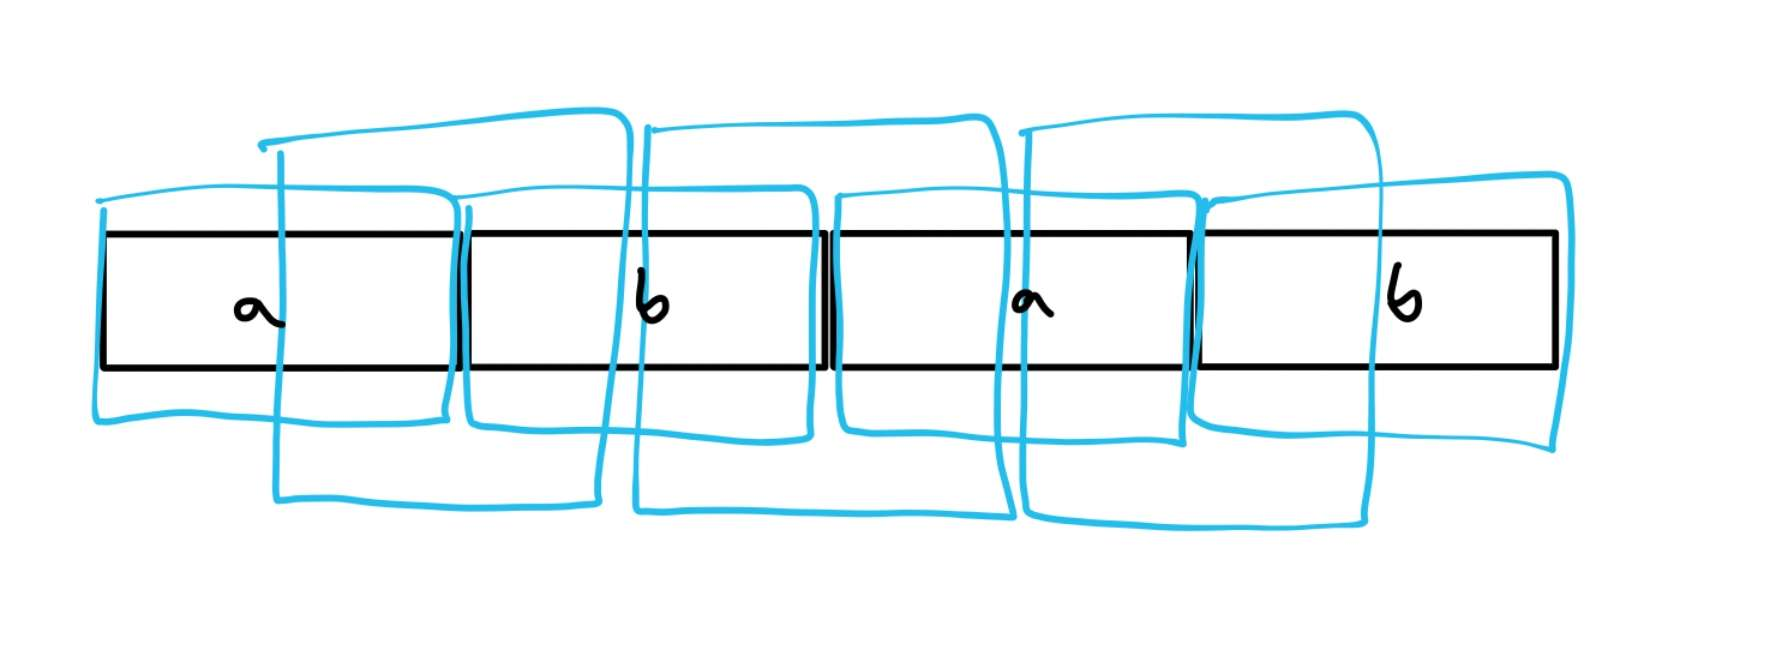
\includegraphics[width=0.3\textwidth]{7moznosti.jpg}
% \end{center}
Takže to dělat nebudeme. 

% pumping lemma intuice: 
% \begin{center}
%     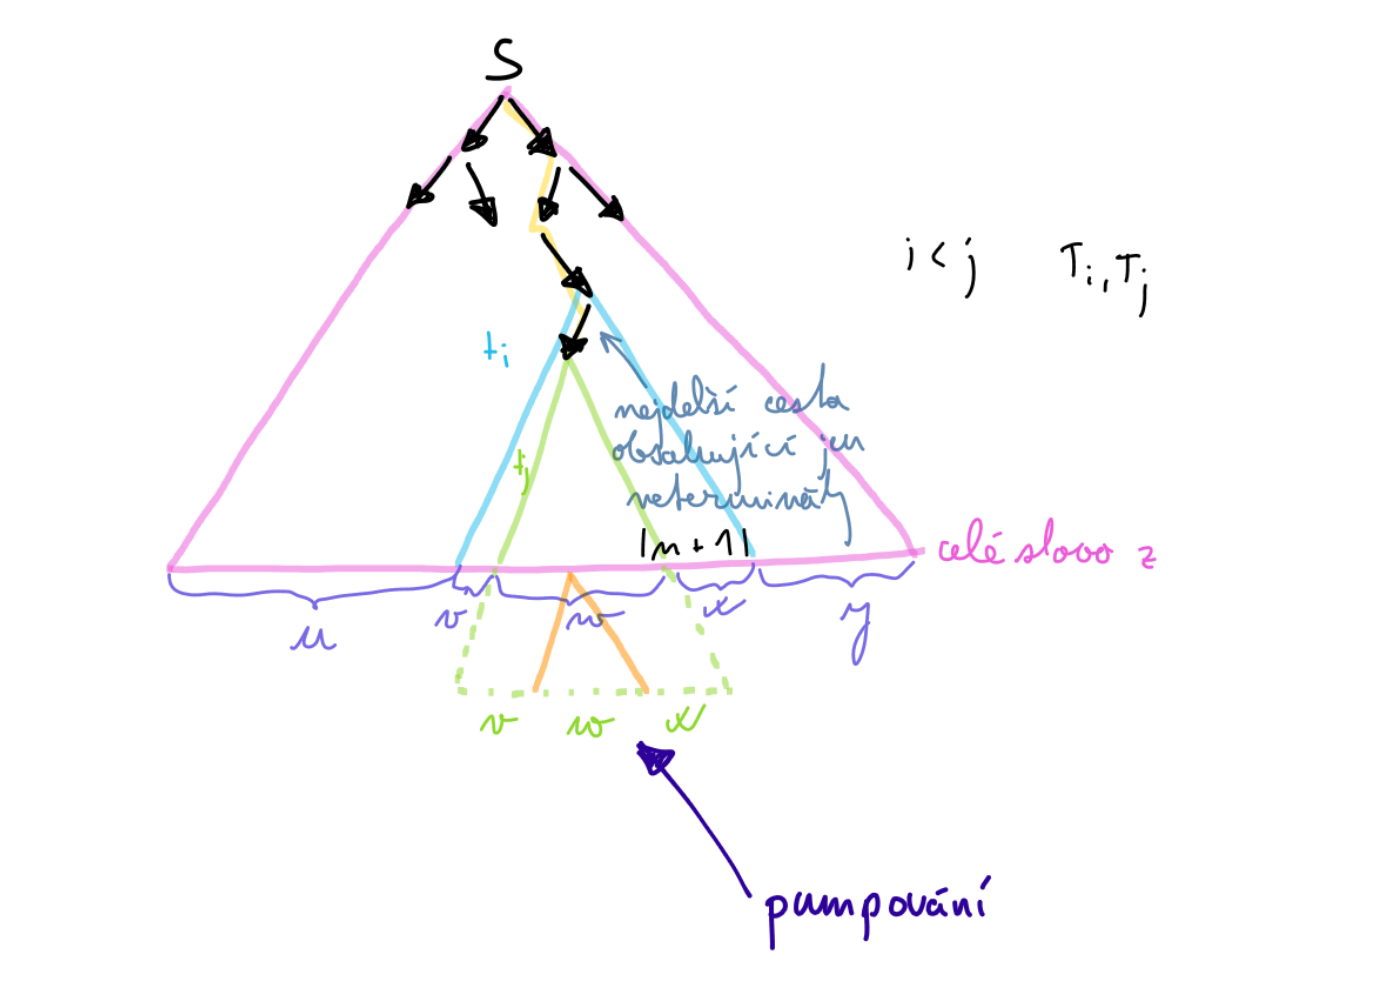
\includegraphics[width=0.5\textwidth]{pl_intuice.png}
% \end{center}

\subsection{Důkaz generování slova matematickou indukcí} % 10.4 
Je dána CF gramatika $\G = (N, \Sigma, S, P)$, kde $N = \{S, A, B, C\}$, $\Sigma = \{a, b\}$ a $P$ je:

\[
\begin{array}{l l}
    P: & S \rightarrow SA \mid aSb \mid Cb \\
       & A \rightarrow SC \mid \varepsilon \\
       & B \rightarrow bAB \mid bS \mid AA \\
       & C \rightarrow CB \mid bA \mid a \\
\end{array}
\]

Pomocí matematické indukce dokažte, že:
\[
A \Rightarrow_{\G}^{\star} S^i A C^i
\]
pro všechna $i \geq 0$. Toho využijte k důkazu, že $(ab)^{i+1}(ab^3)^i$ jsou generována gramatikou $\G$ pro 
každé $i \geq 0$.

1) Základní krok: $i = 0$

Pro $i = 0$ platí:
\[
A {\Longrightarrow^\star} A
\]
což odpovídá:
\[
S^0 A C^0 = A \quad \checkmark
\]

2) Indukční krok:

předp. $A {\implies^\star} S^n A C^n$, chceme dokázat $A \implies^{\star} S^{n+1} A C^{n+1}$.

$A \stackrel{A \rightarrow SC}{\Longrightarrow} SC \stackrel{S \rightarrow SA}{\Longrightarrow} SAC \stackrel{I.P.}
{\Longrightarrow}^{\star} SS^nAC^nC$

nebo

$A \stackrel{I.P.}{\Longrightarrow} S^n A C^n \stackrel{A \rightarrow SC}{\Longrightarrow} S^nSCC^n \stackrel
{S \rightarrow SA}{\Longrightarrow} S^nSACC^n$.



\subsection{Algoritmus CYK} % 10.5 
Je dána gramatika $\G = (N, \Sigma, S, P )$, kde $N = \{S, A, B, C, D\}$, $\Sigma = \{a, b, c\}$ a
pravidla~$P$ jsou dána
\[
\begin{array}{l l}
    P: & S \rightarrow AB \mid CD \mid AC\\
    & A \rightarrow AC \mid a \\
    & B \rightarrow BD \mid b \\
    & C \rightarrow AD \mid a \\
    & D \rightarrow BA \mid b \\ 
\end{array}
\]

Algoritmem CYK rozhodněte, zda gramatika $\G$ generuje slova $w_1$ a $w_2$, kde $w_1 = baaba$ a $w_2 = abaaa$.
 Pokud ano, nakreslete derivační strom a napište jemu odpovídající levou derivaci.


\begin{multicols}{2}
    

\[
    \begin{array}{l l}
    & AB \leftarrow S \\
    & AC \leftarrow S, A \\
    & AD \leftarrow C \\
    & BA \leftarrow D \\
    & BD \leftarrow B \\ 
    & CD \leftarrow S \\ 
    \end{array}
\]
    
slovo $w_1 = baaba$: 

\vspace*{2mm}

\begin{NiceTabular}{ccccc}[hvlines, corners = NE] % NE = north east
    $D$ &  &   &   &   \\ 
    $D$ & $S, A, C$ &  &   &   \\ 
    $D$ & $S, C, A$ & $C, S$ &  &  \\ 
    $D$ & $S, A$ & $S, C$ & $D$ &  \\ 
    $B, D$ & $A,C$ & $A,C$ & $B, D$ & $A, C$ \\ 
\end{NiceTabular}

\hspace*{5mm}$b$ \hspace*{10mm} $a$ \hspace*{10mm} $a$ \hspace*{9mm} $b$ \hspace*{8mm} $a$
    
\vspace*{2mm}
    Gramatika $\G$ negeneruje slovo $w_1$. 

    slovo $w_2 = abaaa$: 
    
    \begin{NiceTabular}{ccccc}[hvlines, corners = NE] % NE = north east
        $C,S$ &   &   &   &   \\ 
        $C, S$ & $D$ &   &   &   \\ 
        $C,S$ & $D$ & $S,A$ &   &   \\ 
        $S,C$ & $D$ & $S,A$ & $S,A$ &   \\ 
        $A,C$ & $B, D$ & $A,C$ & $A,C$ & $A,C$ \\ 
    \end{NiceTabular}
    
\hspace*{5mm}$a$ \hspace*{8mm} $b$ \hspace*{8mm} $a$ \hspace*{8mm} $a$ \hspace*{8mm} $a$


    \vspace*{2mm}
    Gramatika $\G$ generuje slovo $w_2$. 
    
    \columnbreak
    Levá derivace: 
        \begin{align*}
                & S\stackrel{S \rightarrow CD}{\Longrightarrow} CD 
                \stackrel{C \rightarrow a}{\Longrightarrow} aD 
                \stackrel{D \rightarrow BA}{\Longrightarrow} aBA  
                \stackrel{B \rightarrow b}{\Longrightarrow} abA \Longrightarrow\\
                &\stackrel{A \rightarrow AC}{\Longrightarrow} abAC 
                \stackrel{A \rightarrow AC}{\Longrightarrow} abACC 
                \stackrel{A \rightarrow a}{\Longrightarrow} abaCC \Longrightarrow\\
                &\stackrel{C \rightarrow a}{\Longrightarrow} abaaC 
                \stackrel{C \rightarrow a}{\Longrightarrow} abaaa
        \end{align*}
        

    Derivační strom pro slovo $w_2$:
    \begin{center}
        
        \begin{forest}
            for tree={
                grow=south,                 % Tree grows to the right
                edge={->},                  % Draw edges as arrows
                % draw,                       % Draw the nodes
                % rounded corners,           % Rounded corners for nodes
                align=center,                % Center the text inside nodes, 
                }
                [$S$
                    [$C$
                        [$a$]
                    ]
                    [$D$
                        [$B$
                            [$b$]
                        ]
                        [$A$
                            [$A$
                                [$A$
                                    [$a$]
                                ]
                                [$C$
                                    [$a$]
                                ]
                            ]
                            [$C$
                                [$a$]
                            ]
                        ]
                    ]
                ]
            \end{forest}
        \end{center}
\end{multicols}
\section{Jedenácté cvičení}

\subsection{Stavový diagram zásobníkového automatu, práce na automatu}
Je dán zásobníkový automat $A = (Q, \Sigma, \Gamma, \delta, q_0, Z_0, F)$, kde jednotlivé části jsou 
$Q = \bc{q_0, q_1, q_2, q_f}$, $\Sigma = \bc{a, b}$, $\Gamma =\bc{Z_0, X}$ a přechodová funkce je daná tabulkou
\[
\begin{tabular}{|r|c|c|c|c|c|c|}
    \hline
    & $(a, Z_0)$ & $(a, X)$ & $(b, Z_0)$ & $(b, X)$ & $(\varepsilon, Z_0)$ & $(\varepsilon, X)$\\
    \hline
    \hline
    $\rightarrow q_0$& $(q_0, X Z_0)$ & $(q_0, XX)$ & $(q_1, Z_0)$ & $(q_1, \varepsilon)$ & $(q_f, \varepsilon)$ & $-$\\
    $q_1$            & $-$            & $-$         & $(q_1, Z_0)$ & $(q_1, \varepsilon)$ & $(q_f, \varepsilon)$ & $-$\\
    $\leftarrow q_f$ & $-$& $-$& $-$ & $-$ & $-$ & $-$\\
    \hline
\end{tabular}
\]

\begin{enumerate}[a), noitemsep]
    \item Nakreslete stavový diagram zásobníkového automatu $A$.
    \item Ukažte práci zásobníkového automatu nad slovem $aabba$ a slovem $abbbb$.
    \item Charakterizujte jazyk $L$, který tento zásobníkový automat přijímá. Tvrzení zdůvodněte.
\end{enumerate}

\begin{multicols}{2}
    Stavový diagram automatu $A$.

    \begin{tikzpicture}
        \node[state, initial] (0) {$q_0$};
        \node[state, right of=0] (1) {$q_1$};
        \node[state, accepting, below of=0] (f) {$q_f$};

        \draw
            (0) edge[loop above] node[align=center] {$a,Z_0 / X Z_0$ \\ $a,X / XX$} (0)
            (0) edge[bend right, below] node {$b, X / \varepsilon$} (1)
            (0) edge[bend right, above] node {$b, Z_0 / Z_0$} (1)
            (0) edge[bend right, left] node{$\varepsilon, Z_0 / \varepsilon$} (f)
            (1) edge[loop above] node[align=center] {$b,Z_0 / Z_0$ \\ $b,X / \varepsilon$} (1)
            (1) edge[bend left, right] node{$\varepsilon, Z_0 / \varepsilon$} (f)

            ;
    \end{tikzpicture}

\columnbreak

    Práce nad slovem $w_1 = aabba$.

    ${(q_0, aabba, Z_0) \vdash (q_0, abba, X Z_0) \vdash (q_0, bba, XXZ_0)} \vdash (q_1, ba, X Z_0) \vdash (q_1, a, Z_0)$. 
    Konec, neúspěch.

    Práce nad slovem $w_2 = abbbb$.

    $(q_0, abbbb, Z_0) \vdash (q_0, bbbb, X Z_0) \vdash (q_1, bbb, Z_0) \vdash (q_1, bb, Z_0) \vdash (q_1, b, Z_0)
    \vdash (q_1, \varepsilon, Z_0) \vdash (q_f, \varepsilon, \varepsilon)$. \\Konec, úspěch.
\end{multicols}
$L(A) \stackrel{?}{=} \overbrace{\bc{a^i b^j \mid 0 \leq i \leq j}}^L$

Důkaz.

\textbf{a)} $L \subseteq L(A)$
\begin{itemize}[leftmargin=*]
    \item $i=j=0 \text{: } (q_0, \varepsilon, Z_0) \vdash (q_f, \varepsilon, \varepsilon)$
    \item $0=i < j \text{: } (q_0, b^j, Z_0) \vdash (q_1, b^{j-1}, Z_0) \vdash^{(j-1)} (q_1, \varepsilon, Z_0) 
    \vdash (q_f, \varepsilon, \varepsilon)$
    \item ${0<i \leq j \text{: } (q_0, a^i b^j, Z_0) \vdash^i (q_0, b^{i+k}, X^i Z_0) \vdash (q_0, b^{i+k-1}, X^{i-1} Z_0)
    \vdash^{(i-1)} (q_1, b^k, Z_0) \vdash^k (q_1, \varepsilon, Z_0) \vdash (q_f, \varepsilon, \varepsilon),}\\
    i+k = j, k=j-i \geq 0$.
\end{itemize}
\textbf{b)} $L(A) = N(A) \subseteq L$

Dokazujeme, že pokud $w \in L(A)$, pak $w$ má tvar $a^i b^j$, kde $0 \leq i \leq j$. Pro $w \in L(A)$ musí zásobníkový 
automat $A$ skončit ve stavu $q_f$ s prázdným vstupním řetězcem i zásobníkem.
\begin{itemize}[leftmargin=*]
    \item Přidávání $a$:
    Každý symbol $a$ způsobí, že do zásobníku přidáme jeden symbol $X$. Zásobník tak obsahuje $i$ symbolů $X$ po 
    zpracování $a^i$.
    \item Zpracování $b$:
    Každý symbol $b$ odstraní jeden symbol $X$ ze zásobníku, pokud je tam ještě přítomen. Pokud už jsou všechny $X$ 
    odstraněny, symbol $b$ pouze projde automatem, aniž by zásobník změnil svůj stav.
    \item Prázdný zásobník:
    Stav $q_f$ je přístupný pouze tehdy, když je zásobník prázdný. To znamená, že každý přidaný $X$ odpovídá 
    odstraněnému $X$, což nastane právě tehdy, když $i \leq j$.
\end{itemize}
Z toho plyne, že $w = a^i b^j$ s $0 \leq i \leq j$.

\section{Dvanácté cvičení}

\subsection{Tvorba zásobníkového automatu podle jazyka}
Je dán jazyk $L$ nad abecedou $\Sigma = \{a,b\}$. Sestrojte zásobníkové automaty $A,B$ tak, že $L = N(A)$ a $L = L(B)$ 
(tj. $A$ přijímá $L$ prázdným zásobníkem, $B$ přijímá $L$ koncovým stavem), kde
\[L = \{(ab)^i b^j a^{j-i} \mid 0 < i < j\}\text{.}\]

$\implies L= \{(ab)^i b^{i+k} a^k \mid i>0, k>0\} \implies N(A)=\underbrace{\{(ab)^i b^i \mid k>0\}}_X,
L(B)=\underbrace{\{b^k a^k \mid k>0\}}_Y$.

Dva způsoby řešení:

a) Přímo.

\begin{tikzpicture}
    \node[state, initial] (0) {$q_0$};
    \node[state, right of=0] (1) {$q_1$};
    \node[state, right of=1] (2) {$q_2$};
    \node[state, right of=2] (3) {$q_3$};
    \node[state, right of=3] (4) {$q_4$};
    \node[state, right of=4] (5) {$q_5$};
    \node[state, accepting, below of=5] (f) {$q_f$};

    \draw
        (0) edge[bend left, above] node{$a, Z_0 / Z_0$} (1)
        (1) edge[bend left, above] node[align=center] {$b, Z_0 / X Z_0$ \\ $b, X / XX$} (2)
        (2) edge[bend left, above] node{$b, X / \varepsilon$} (3)
        (2) edge[bend left, below] node{$a, X / X$} (1)
        (3) edge[loop above] node{$b, X / \varepsilon$} (3)
        (3) edge[bend left, above] node{$b, Z_0 / Y Z_0$} (4)
        (4) edge[loop above] node{$b, Y / YY$} (4)
        (4) edge[bend left, above] node{$a, Y / \varepsilon$} (5)
        (5) edge[loop above] node{$a, Y / \varepsilon$} (5)
        (5) edge[bend left, left] node{$\varepsilon, Z_0 / \varepsilon$} (f)
        ;
\end{tikzpicture}

b) Přes gramatiku.
\begin{multicols}{3}
    \raggedcolumns
    \begin{flalign*}
        \G: S &\rightarrow AB &\\
        A &\rightarrow abAb \mid abb &\\
        B &\rightarrow bBa \mid ba &
    \end{flalign*}

\columnbreak

    Prázdným zásobníkem: 
    \[
    \begin{array}{l l}
        & \delta(q, \varepsilon, S) = \{(q, AB)\} \\
        & \delta(q, \varepsilon, A) = \{(q, abAb), (q, abb)\} \\
        & \delta(q, \varepsilon, B) = \{(q, bBa), (q, ba)\} \\
        & \delta(q, a, a) = \{(q, \varepsilon)\} \\
        & \delta(q, b, b) = \{(q, \varepsilon)\} \\ 
    \end{array}
    \]
    

    Koncovým stavem: 
    \[
    \begin{array}{l l}
        & \delta(q_0, \varepsilon, Z_0) = \{(q, SZ_0)\} \\
        & \delta(q, \varepsilon, S) = \{(q, AB)\} \\
        & \delta(q, \varepsilon, A) = \{(q, abAb), (q, abb)\} \\
        & \delta(q, \varepsilon, B) = \{(q, bBa), (q, ba)\} \\
        & \delta(q, a, a) = \{(q, \varepsilon)\} \\
        & \delta(q, b, b) = \{(q, \varepsilon)\} \\ 
        & \delta(q, \varepsilon, Z_0) = \{(q_f, \varepsilon)\} \\ 
    \end{array}
    \]
\end{multicols}

\noindent
1. $L \subseteq L(G)$\\
$S \xRightarrow{S \rightarrow AB} AB \xRightarrow{A \rightarrow abAb}^{(i-1)} (ab)^{i-1} A b^{i-1} B \xRightarrow{A \rightarrow abb}
(ab)^i b^i B \xRightarrow{B \rightarrow bBa}^{(k-1)} (ab)^i b^i b^{k-1} B a^{k-1} \xRightarrow{B \rightarrow ba} (ab)^i b^i b^k a^k$.

\noindent
2. $L(G) \subseteq L$\\ % TODO: dodělat důkaz
$S \rightarrow^\star w$\\
$S \rightarrow AB$\\
$A \xRightarrow{A \rightarrow abAb}^j (ab)^j A b^j \xRightarrow{A \rightarrow abb} (ab)^j a b b^j$

\subsection{Tvorba zásobníkového automatu podle jazyka}
Je dán jazyk $L$ nad abecedou $\Sigma = \{a,b\}$. Sestrojte zásobníkové automaty $A,B$ tak, že $L = N(A)$ a $L = L(B)$ 
(tj. $A$ přijímá $L$ prázdným zásobníkem, $B$ přijímá $L$ koncovým stavem), kde
\[L = \{w \mid w \text{ začíná a končí symbolem } 1 \text{ a obsahuje o dvě } 1 \text{ více než } 0\}\text{.}\]

$L = \{1u1 \mid |u|_0 = |u|_1\}, i = |u|_0$

\begin{tikzpicture}
    \node[state, initial] (0) {$q_0$};
    \node[state, right of=0] (1) {$q_1$};
    \node[state, accepting, right of=1] (f) {$q_f$};
    
    \draw
        (0) edge[bend left, above] node{$1, Z_0 / Z_0$} (1)
        (1) edge[loop above] node[align=center]{$0, Z_0 / 0 Z_0$\\$1, Z_0 / 1 Z_0$} (1)
        (1) edge[loop below] node[align=center]{$0,0 / 00$\\ $1,1 / 11$\\ $0,1 / \varepsilon$\\ $1,0 / \varepsilon$} (1)
        (1) edge[bend left, above] node{$1, Z_0 / \varepsilon$} (f)
        ;
\end{tikzpicture}

\textbf{1)} $L \subseteq N(A)$

$(q_0, 1u1, Z_0) \vdash (q_1, u1, Z_0) \vdash^\star (q_1, 1, Z_0) \vdash (q_f, \varepsilon, \varepsilon)$.

\textbf{2)} $L(B) \subseteq L$

Musíme ukázat, že pokud zásobníkový automat $B$ přijme slovo $w$, pak $w \in L$. To znamená, že $w$ začíná a končí 
symbolem $1$ a obsahuje o dvě více symbolů $1$ než $0$.

Vlastnosti přechodů:
\begin{enumerate}[noitemsep]
    \item Automat přechází z počátečního stavu $q_0$ do $q_1$, pokud první symbol je $1$. Tuto $1$ nezapočítáme.
    \item Ve stavu $q_1$ se zásobníkem automat udržuje informaci o rozdílu mezi počtem symbolů $1$ a $0$:
    \begin{itemize}[noitemsep]
        \item Při čtení symbolů $0$ a $1$ přidává, respektive odstraní (pokud existuje) odpovídající značku do zásobníku,
        což udržuje informaci o tom, zda je stejný počet obou znaků.
    \end{itemize}
    \item Pokud zpracování skončí symbolem $1$ a zásobník je prázdný, automat přejde do koncového stavu $q_f$, což 
    zajišťuje, že rozdíl mezi počtem symbolů $1$ a $0$ je přesně dvě.
\end{enumerate}
Každé slovo přijaté automatem $B$ splňuje podmínky:
\begin{itemize}[noitemsep]
    \item Začíná symbolem $1$ (nutný přechod z $q_0$ do $q_1$).
    \item Končí symbolem $1$ (nutný přechod z $q_1$ do $q_f$).
    \item Obsahuje přesně o dvě více symbolů $1$ než $0$ (zásobník na konci zajišťuje prázdný stav).
\end{itemize}
Z toho plyne, že $L(B) \subseteq L$.

\subsection{Tvorba zásobníkového automatu podle jazyka}
Je dán jazyk $L$. Sestrojte zásobníkové automaty $A$, $B$ tak, že $L = N(A)$ a $L = L(B)$ (tj. $A$ přijímá $L$ prázdným 
zásobníkem, $B$ přijímá $L$ koncovým stavem), kde $$L = \{a^i b^i c^{i+j}\}$$
Ukažte práci nad slovem $w = abcc$. 

Konstrukce pomocí gramatiky: 

$\medskip S \to aSc \mid A$\\
$\medskip A \to bAc \mid \varepsilon$

\begin{multicols}{2}
    
    Prázdným zásobníkem: 
    \[
    \begin{array}{l l}
        & \delta(q, \varepsilon, S) = \{(q, aSc), (q, A)\} \\
        & \delta(q, \varepsilon, A) = \{(q, bAc), (q, \varepsilon)\} \\
        & \delta(q, a, a) = \{(q, \varepsilon)\} \\
        & \delta(q, b, b) = \{(q, \varepsilon)\} \\ 
        & \delta(q, c, c) = \{(q, \varepsilon)\} \\ 
    \end{array}
    \]

    Práce nad slovem $w = abcc$:

    $
    {(q, abbc, S) \vdash (q, abcc, aSc) \vdash (q, bcc, Sc) \vdash}\\
    {(q, bcc, Ac) \vdash (q, bcc, bAcc) \vdash (q, cc, Acc) \vdash}\\ 
    {(q, cc, cc) \vdash (q, c, c) \vdash(q, \varepsilon, \varepsilon)}
    $

\columnbreak

    Koncovým stavem: 
    \[
    \begin{array}{l l}
        & \delta(q_0, \varepsilon, Z_0) = \{(q, SZ_0)\} \\
        & \delta(q, \varepsilon, S) = \{(q, AB)\} \\
        & \delta(q, \varepsilon, A) = \{(q, abAb), (q, abb)\} \\
        & \delta(q, \varepsilon, B) = \{(q, bBa), (q, ba)\} \\
        & \delta(q, \varepsilon, a) = \{(q, \varepsilon)\} \\
        & \delta(q, \varepsilon, b) = \{(q, \varepsilon)\} \\ 
        & \delta(q, \varepsilon, Z_0) = \{(q_f, \varepsilon)\} \\ 
    \end{array}
    \]

    Práce nad slovem $w = abcc$:

    $
    {(q_0, abc, Z_0) \vdash (q, abbc, SZ_0) \vdash (q, abcc, aScZ_0) \vdash}\\
    {(q, bcc, SZ_0c) \vdash (q, bcc, AcZ_0) \vdash (q, bcc, bAccZ_0) \vdash}\\
    {(q, cc, AccZ_0) \vdash ( q, cc, ccZ_0) \vdash (q, c, cZ_0) \vdash}\\
    (q, \varepsilon, Z_0) \vdash (q_f, \varepsilon, \varepsilon)
    $
\end{multicols}

\subsection{Důkaz bezkontextovosti jazyka}
Je dán jazyk $L = \{0^n 1^m; 0 \leq n \leq m \leq 2n\}$. Rozhodněte, zda jazyk $L$ je bezkontextový.\\
V případě, že je bezkontextový, najděte buď bezkontextovou gramatiku, která ho generuje, nebo zásobníkový automat, který 
ho přijímá.\\
V případě, že není bezkontextový, tvrzení dokažte.

Například $\G$ s pravidly $P$:
\begin{flalign*}
    S \rightarrow 0S11 \mid 0S1 \mid \varepsilon & \\
\end{flalign*}
Důkaz.

\textbf{1)} $L \subseteq L(\G)$ $-$ $\G$ generuje celé $L$
\begin{itemize}[leftmargin=*]
    \item $0 < n \leq m \leq 2n \rightarrow k=2n-m \geq 0$:\\
    $S \xRightarrow{S \rightarrow 0S1}^{(k)} 0^k S 1^k \xRightarrow{S \rightarrow 0S11}^{(n-k)} 0^k 0^{n-1} S 1^{n-1} 
    1^{n-1} 1^k \xRightarrow{S \rightarrow \varepsilon} 0^n 1^{2n-k} = 0^n 1^{2n - 2n + m} = 0^n 1^m$.
    \item $0 = n = m$: $ 0^0 1^0 = \varepsilon \in L$.
\end{itemize}
\textbf{2)} $L(\G) \subseteq L$ $-$ $\G$ negeneruje nic navíc

Nechť $w \in L(\G)$, kde $w = 0^n 1^m$. Sledujeme pravidla gramatiky $\G$:

(0) základní krok: Pokud $S \rightarrow \varepsilon$, pak $w = \varepsilon = 0^0 1^0$. Zřejmě $\varepsilon \in L$.

(1) indukční krok: 
\begin{itemize}
    \item Pokud $S \rightarrow 0S1$, přidáváme jeden symbol $0$ na začátek a jeden symbol $1$ na konec. Po aplikaci 
    tohoto pravidla se počet $0$ zvýší o jeden a počet $1$ o jedna, tedy platí $n \leq m \leq 2n$.
    \item Pokud $S \rightarrow 0S11$, přidáváme jeden symbol $0$ na začátek a dva symboly $1$ na konec. Po aplikaci 
    tohoto pravidla se počet $0$ zvýší o jeden a počet $1$ o dva, tedy stále platí $n \leq m \leq 2n$.
\end{itemize}


%%% Ugly hack for no spacing around alignments, just a local thing
\setlength{\abovedisplayskip}{0pt}
\setlength{\belowdisplayskip}{0pt}
\setlength{\abovedisplayshortskip}{0pt}
\setlength{\belowdisplayshortskip}{0pt}
%%%

\section{Třinácté cvičení}

\subsection{Tvorba a práce zásobníkového automatu podle jazyka}
Je dán jazyk $L$ nad abecedou $\Sigma = \{0,1\}$. Sestrojte zásobníkové automaty $A,B$ tak, že $L = N(A)$ a $L = L(B)$
(tj. $A$ přijímá $L$ prázdným zásobníkem, $B$ přijímá $L$ koncovým stavem), kde
\[L = \{0^i 1^j 0^k \mid 0 \leq i < k, j > 0\}\text{.}\]
Ukažte práci jednoho ze zásobníkových automatů nad slovem $011000$ a nad slovem $001110$.

Přímou metodou:

\begin{multicols}{2}
    \begin{tikzpicture}
        \node[state, initial] (0) {$q_0$};
        \node[state, right of=0] (1) {$q_1$};
        \node[state, right of=1] (2) {$q_2$};
        \node[state, accepting, below of=1] (f) {$q_f$};

        \draw
            (0) edge[loop above] node[align=center]{$0, A / AA$ \\ $0, Z_0 / A Z_0$} (0)
            (0) edge[bend left, above] node{$1, Z_0 / Z_0$} (1)
            (0) edge[bend left, below] node{$1, A / A$} (1)
            (1) edge[loop above] node[align=center]{$1, A / A$ \\ $1, Z_0 / Z_0$} (1)
            (1) edge[bend left, above] node{$0, Z_0 / Z_0$} (2)
            (1) edge[bend left, below] node{$0, A / A$} (2)
            (2) edge[loop above] node[align=center]{$0, A / \varepsilon$ \\ $0, Z_0 / Z_0$} (2)
            (2) edge[bend left, left] node{$\varepsilon, Z_0 / \varepsilon$} (f)
            ;
  \end{tikzpicture}

    \columnbreak\

    Práce nad slovem $w_1 = 011000$.

    ${(q_0, 011000, Z_0) \vdash (q_0, 11000, A Z_0) \vdash (q_1, 1000, A Z_0)}$
    \begin{flalign*}
        \vdash (q_1, 000, A Z_0) \vdash (q_2, 00, A Z_0) &\vdash (q_f, 0, A Z_0) \xmark & \\
        &\vdash (q_2, 0, Z_0)
    \end{flalign*}
    \begin{flalign*}
        (q_2, 0, Z_0) &\vdash (q_f, 0, Z_0) \xmark & \\
        &\vdash (q_2, \varepsilon, Z_0) \vdash (q_f, \varepsilon, \varepsilon) \checkmark
    \end{flalign*}

    Práce nad slovem $w_2 = 001110$.

    ${(q_0, 001110, Z_0) \vdash^{(2)} (q_0, 1110, AA Z_0) \vdash} \\
    (q_1, 110, AA Z_0) \vdash^{(2)} (q_1, 0, AA Z_0) \vdash (q_2, \varepsilon, AA Z_0) \xmark $

\end{multicols}

Přes gramatiku:
\begin{flalign*}
    \G : S &\rightarrow S0 \mid 0S0 \mid A0 & \\
    A &\rightarrow 1A \mid 1
\end{flalign*}

Důkaz.

1) $L \subseteq L(\G)$\\
$S \Rightarrow^\star 0^i S 0^k \xRightarrow{S \rightarrow A0} 0^i A 0^{k+1} \xRightarrow{A \rightarrow 1A}^{(j)}
0^i 1^j A 0^{k+1} \xRightarrow{A \rightarrow 1} 0^i 1^{j+1} 0^{k+1}$, $i \leq k, j > 0$. %? Is this in the right spot?

2) $L(\G) \subseteq L$\\ % TODO: dodělat důkaz

\subsection{Tvorba nevypouštěcí gramatiky}
Je dána bezkontextová gramatika $\G = (N, \Sigma, S, P)$, kde $N = \{S,A,B,C\}, \Sigma = \{0,1\}$ a $P$ je dáno
\begin{align*}
    S &\rightarrow SA \mid 0 \\
    A &\rightarrow BAB \mid 1 \\
    B &\rightarrow CB \mid \varepsilon \\
    C &\rightarrow AS \mid 0 \mid \varepsilon
\end{align*}
Ke gramatice $\G$ vytvořte nevypouštěcí gramatiku $\G_1$. V gramatice $\G_1$ odstraňte levou rekurzi.

\textbf{1. krok} Vytvoření nevypouštěcí gramatiky $\G_1$.
\begin{multicols}{2}
    \begin{flalign*}
        V &= \{x \mid x \Rightarrow^\star \varepsilon\} & \\
        V_1 &= \{x \mid x \rightarrow \varepsilon \in P\} = \{B,C\} & \\
        V_2 &= V_1 \cup \{x \mid x \rightarrow \alpha \in P, \alpha \in V_1^+\} = V_1 \cup \emptyset = V_1 = V.
    \end{flalign*}

\columnbreak

    \begin{flalign*}
        P^{'} \text{: } S &\rightarrow SA \mid 0 & \\
        A &\rightarrow BAB \mid AB \mid BA \mid A \mid 1 & \\
        B &\rightarrow CB \mid C & \\
        C &\rightarrow AS \mid 0
    \end{flalign*}
\end{multicols}
\textbf{2. krok} odstranění levé rekurze. (postup shora dolů)
\begin{flalign*}
    S^{\phantom{'}}    &\rightarrow 0 \mid 0S^{'} & \\
    S^{'}&\rightarrow A \mid AS^{'} & \\
    A^{\phantom{'}}    &\rightarrow BAB \mid BA \mid 1 \mid BABA^{'} \mid BAA^{'} \mid 1A^{'} & \\
    A^{'}&\rightarrow B \mid BA^{'} & \\
    B^{\phantom{'}}    &\rightarrow CB \mid C & \\
    C^{\phantom{'}}    &\rightarrow AS \mid 0
\end{flalign*}

\vspace*{-2mm}

\subsection{Převod gramatiky do Greibachové normální formy}
Do Greibachové normální formy převěďte gramatiku $\G$, kde $\G = (N, \Sigma, S, P)$, kde $N = \{S, E, F\},\\
\Sigma = \{a, *, +, ), (\}$ a $P$ je dáno
\begin{align*}
    S &\rightarrow (E)\\
    E &\rightarrow F * F \mid F + F\\
    F &\rightarrow a \mid S
\end{align*}
\textbf{1. krok} oindexování neterminálů.\\
$A_1 = S \\
A_2 = E \\
A_3 = F
$

\textbf{2. krok} odstranění levých rekurzí. Kontrola správného pořadí indexů (na pravé straně vždy neterminál s větším
indexem), jinak sloučit pravidla. (postup shora dolů)
\begin{flalign*}
    S &\rightarrow (E) & \\
    E &\rightarrow F * F \mid F + F& \\
    F &\rightarrow a \mid (E)
\end{flalign*}

\textbf{3. krok} nahrazení prvních neterminálů pravých stran, které neterminálem začínají, pravidly. (postup zespoda
nahoru)
\begin{flalign*}
    S &\rightarrow (E) & \\
    E &\rightarrow a * F \mid a + F \mid (E) * F \mid (E) + F& \\
    F &\rightarrow a \mid (E)
\end{flalign*}

\textbf{4. krok} za prvním terminálem pravé strany vždy následují pouze neterminály.
\begin{flalign*}
    S &\rightarrow (EX & \\
    E &\rightarrow a Y F \mid a Z F \mid (EX Y F \mid (EX Z F & \\
    F &\rightarrow a \mid (EX & \\
    X &\rightarrow ) & \\
    Y &\rightarrow * & \\
    Z &\rightarrow +
\end{flalign*}

\subsection{Převod gramatiky do Greibachové normální formy}
Do Greibachové normální formy převěďte gramatiku $\G$, kde $\G = (N, \Sigma, S, P)$, kde $N = \{S, A, B\},\\
\Sigma = \{a, b, c\}$ a $P$ je dáno
\begin{align*}
    S &\rightarrow Ab \mid B\\
    A &\rightarrow Aba \mid Bcc\\
    B &\rightarrow Sa \mid b
\end{align*}
\textbf{1. krok} oindexování neterminálů.\\
$A_1 = S \\
A_2 = A \\
A_3 = B$

\textbf{2. krok} odstranění levých rekurzí. Kontrola správného pořadí indexů (na pravé straně vždy neterminál s větším
indexem), jinak sloučit pravidla. (postup shora dolů)
\begin{flalign*}
    S^{\phantom{'}} &\rightarrow Ab \mid B & \\
    A^{\phantom{'}} &\rightarrow Ba \mid BaA^{'} & \\
    A^{'} &\rightarrow ba \mid baA^{'} & \\
    B^{\phantom{'}} &\rightarrow Aba \mid Ba \mid b & \\
    B^{\phantom{'}} &\rightarrow Baba \mid BaA^{'}ba \mid Ba \mid b & \\
    B^{\phantom{'}} &\rightarrow b \mid bB^{'} & \\
    B^{'} &\rightarrow aba \mid aA^{'}ba \mid a \mid abaB^{'} \mid aA^{'}baB^{'} \mid aB^{'}
\end{flalign*}

\textbf{3. krok} nahrazení prvních neterminálů pravých stran, které neterminálem začínají, pravidly. (postup zespoda
nahoru)
\begin{flalign*}
    S^{\phantom{'}} &\rightarrow Bab \mid BaA^{'} \mid b \mid bB^{'} & \\
    A^{\phantom{'}} &\rightarrow ba \mid bB^{'}a \mid baA^{'} \mid bB^{'}aA^{'} & \\
    A^{'} &\rightarrow ba \mid baA^{'} & \\
    B^{\phantom{'}} &\rightarrow b \mid bB^{'} & \\
    B^{'} &\rightarrow aba \mid aA^{'}ba \mid a \mid abaB^{'} \mid aA^{'}baB^{'} \mid aB^{'}
\end{flalign*}

\textbf{4. krok} za prvním terminálem pravé strany vždy následují pouze neterminály.
\begin{flalign*}
    S^{\phantom{'}} &\rightarrow BaY \mid BaA^{'} \mid b \mid bB^{'} & \\
    A^{\phantom{'}} &\rightarrow bX \mid bB^{'}X \mid bXA^{'} \mid bB^{'}aA^{'} & \\
    A^{'} &\rightarrow bX \mid bXA^{'} & \\
    B^{\phantom{'}} &\rightarrow b \mid bB^{'} & \\
    B^{'} &\rightarrow aXY \mid aA^{'}YX \mid a \mid aYXB^{'} \mid aA^{'}YXB^{'} \mid aB^{'} & \\
    X^{\phantom{'}} &\rightarrow a & \\
    Y^{\phantom{'}} &\rightarrow b
\end{flalign*}
\section{Čtrnácté cvičení}

\subsection{Převod gramatiky do Greibachové normální formy}
Do Greibachové normální formy převeďte gramatiku $\G$, kde $\G = (N, \Sigma, S, P)$, kde $N = \bc{S, A}$, 
\\$\Sigma = \bc{0, 1}$ a $P$ je dáno
\begin{align*}
    S &\rightarrow SA \mid 0 \\
    A &\rightarrow AS \mid 1
\end{align*} 

\textbf{1. krok} oindexování neterminálů.

$X_1 = S \\
X_2 = A \\
X_3 = S^{'} \\
X_4 = A^{'}
$

\textbf{2. krok} odstranění levých rekurzí.
\begin{flalign*}
    S^{\phantom{'}} &\rightarrow 0 \mid 0S^{'} & \\
    S^{'} &\rightarrow A \mid AS^{'} & \\
    A^{\phantom{'}} &\rightarrow 1 \mid 1A^{'} & \\
    A^{'} &\rightarrow S \mid SA^{'} &
\end{flalign*}

\textbf{3. krok} Kontrola správného pořadí indexů (na pravé straně vždy neterminál s větším 
indexem), jinak sloučit pravidla. (postup shora dolů)
\begin{flalign*}
    S^{\phantom{'}} &\rightarrow 0 \mid 0S^{'} & \\
    A^{\phantom{'}} &\rightarrow 1 \mid 1A^{'} & \\
    S^{'} &\rightarrow 1 \mid 1A^{'} \mid 1S^{'} \mid 1A^{'}S^{'}  & \\
    A^{'} &\rightarrow 0 \mid 0S^{'} \mid 0A^{'} \mid 0S^{'}A^{'} &
\end{flalign*}

\textbf{4. krok} za prvním terminálem pravé strany vždy následují pouze neterminály. $\checkmark$

\subsection{Zkoušková ukázka práce na bezkontextové gramatice}
Je dána bezkontextová gramatika $\G = (N, \Sigma, S, P)$, kde $N = \bc{S,A,B,C}$, $\Sigma = \bc{a,b}$ a $P$ je dáno

\begin{align*}
    S &\rightarrow Sa \mid Sb \mid bC \\
    A &\rightarrow CBA \mid BC \mid b \\
    B &\rightarrow aB \mid \varepsilon \\
    C &\rightarrow AA \mid bBb \mid \varepsilon
\end{align*}

\begin{enumerate}[noitemsep]
    \item Ke gramatice $\G$ najděte nevypouštěcí gramatiku $\G_1$. Kroky převodu popište.
    \item Ke gramatice $\G_1$ najděte gramatiku $\G_2$ v Chomského normálním tvaru, která generuje stejný jazyk jako 
    gramatika $\G_1$. Jednotlivé kroky popište, gramatiku v Chomského normálním tvaru definujte.
    \item Pomocí matematické indukce dokažte, že platí $A \Rightarrow_\G^\star A^i C (BA)^{i+1}$ pro každé $i \geq 0$.
    Toho využijte k důkazu, že $b^{i+2}(ab)^{i+1}$ je generováno gramatikou $\G$ pro každé $i \geq 0$.
    \item Je gramatika $\G$ víceznačná? Víceznačnou gramatiku definujte.
    \item V gramatice $\G_1$ odstraňte levou rekurzi u symbolu $S$. Postup popište.
\end{enumerate}

\textbf{1.} Nevypouštěcí gramatika $\G_1$. 

$V = \bc{A \mid A \Rightarrow^\star \varepsilon }$\\
$V_1 = \bc{A \mid A \rightarrow \varepsilon \in P} = \bc{B, C}$\\
$V_2 = V_1 \cup \bc{A \mid A \rightarrow \alpha \in P, \alpha \in V_1^{\star}} = V_1 \cup \bc{A} = \bc{A, B, C}$\\
$V_3 = V_2 \cup \bc{A \mid A \rightarrow \alpha \in P, \alpha \in V_2^{\star}} = V_2 \cup \varepsilon = V_2 = V$

\begin{flalign*}
    \G_1: S &\rightarrow Sa \mid Sb \mid bC \mid b & \\
    A &\rightarrow CBA \mid CA \mid CB \mid BA \mid BC \mid B \mid C \mid b & \\
    B &\rightarrow aB \mid a & \\
    C &\rightarrow AA \mid A \mid bBb \mid bb &
\end{flalign*}

\textbf{2.} Chomského normální tvar gramatiky $\G_1$.

\textbf{1. krok} nahrazení samostatných terminálů pravidly. (pokud nastane např. $A \rightarrow A$, tak vynechat.)
\begin{flalign*}
    S &\rightarrow Sa \mid Sb \mid bC \mid b & \\
    A &\rightarrow CBA \mid CA \mid CB \mid BA \mid BC \mid \underbrace{aB \mid a}_B \mid \underbrace{AA \mid bBb \mid bb}_C \mid b & \\
    B &\rightarrow aB \mid a & \\
    C &\rightarrow AA \mid \underbrace{CBA \mid CA \mid CB \mid BA \mid BC \mid B \mid C \mid b}_A \mid bBb \mid bb &
\end{flalign*}

\textbf{2. krok} nahrazení terminálů neterminály pokud nejsou samotné.
\begin{flalign*}
    S &\rightarrow SX_1 \mid SX_2 \mid X_2C \mid b & \\
    A &\rightarrow CBA \mid CA \mid CB \mid BA \mid BC \mid X_1B \mid X_1 \mid AA \mid X_2BX_2 \mid X_2X_2 \mid X_2 & \\
    B &\rightarrow X_1B \mid X_1 & \\
    C &\rightarrow AA \mid CBA \mid CA \mid CB \mid BA \mid BC \mid B \mid C \mid X_2 \mid X_2BX_2 \mid X_2X_2 & \\
    X_1 &\rightarrow a & \\
    X_2 &\rightarrow b & \\
\end{flalign*}

\textbf{3. krok} nahrazení pravých stran, která mají délku $\geq 3$.
\begin{flalign*}
    S &\rightarrow SX_1 \mid SX_2 \mid X_2C \mid b & \\
    A &\rightarrow Y \mid CA \mid CB \mid BA \mid BC \mid X_1B \mid X_1 \mid AA \mid Z \mid X_2X_2 \mid X_2 & \\
    Y &\rightarrow CBA & \\
    Z &\rightarrow X_2BX_2 & \\
    B &\rightarrow X_1B \mid X_1 & \\
    C &\rightarrow AA \mid Y \mid CA \mid CB \mid BA \mid BC \mid B \mid C \mid X_2 \mid Z \mid X_2X_2 & \\
    X_1 &\rightarrow a & \\
    X_2 &\rightarrow b & \\
\end{flalign*}

\textbf{3.} Důkaz.

$A \Rightarrow_\G^\star A^i C (BA)^{i+1}$

Základní krok: $i=0$: $A^0 C (BA)^1 = CBA$ $\checkmark$ $A \Rightarrow_\G^\star CBA$.

Indukční krok: $i \geq 0$: indukční předpoklad: $A \Rightarrow^\star A^i C (BA)^{i+1}$.

$A \xRightarrow{A \rightarrow CBA} CBA \xRightarrow{C \rightarrow AA} A\underline{A}_{IP} (BA) \xRightarrow{IP}^\star 
AA^i C (BA)^{i+1} (BA) = A^{i+1} C (BA)^{i+2}$. $\checkmark$

A tedy, $b^{i+2} (ab)^{i+1} \in L(\G)$?

$S \xRightarrow{S \rightarrow bC} bC \xRightarrow{C \rightarrow AA} bAA \xRightarrow{A \rightarrow b} b^2 A \Rightarrow
|\text{dle důkazu výše}| \xRightarrow{}^\star b^2 A^i C (BA)^{i+1} \xRightarrow{A \rightarrow b} b^{i+2} C (BA)^{i+1} 
\xRightarrow{C \rightarrow \varepsilon} b^{i+2} (BA)^{i+1} \xRightarrow{B \rightarrow aB} b^{i+2} (aBA)^{i+1} 
\xRightarrow{B \rightarrow \varepsilon} b^{i+2} (aA)^{i+1} \xRightarrow{A \rightarrow b} b^{i+2} (ab)^{i+1}$. $\checkmark$

\textbf{4.} Je gramatika $\G$ víceznačná?

Víceznačnost = existují alespoň 2 derivační stromy / 2 levé derivace pro jedno libovolné slovo z $\G$.

Například mějme slovo $w=bbb$.

První způsob vygenerování slova $w$: $S \xRightarrow{S \rightarrow bC} bC \xRightarrow{C \rightarrow AA} bAA
\xRightarrow{A \rightarrow b}^2 bbb.$

Druhý způsob vygenerování slova $w$: $S \xRightarrow{S \rightarrow bC} bC \xRightarrow{C \rightarrow bBb} bbBb
\xRightarrow{B \rightarrow \varepsilon} bbb.$

A tedy gramatika $\G$ je víceznačná.

\textbf{5.} Odstranění levých rekurzí.

Levá rekurze se vyskytuje pouze v pravidlu $S \rightarrow Sa \mid Sb \mid bC \mid b$.

Je potřeba přidat pouze jeden neterminál. Pokud by se jich přidalo více, nová gramatika by generovala méně slov, než původní.
\begin{flalign*}
    S^{\phantom{'}} &\rightarrow bC \mid bCS^{'} \mid b \mid S^{'} & \\
    S^{'} &\rightarrow a \mid aS^{'} \mid b \mid bS^{'} &
\end{flalign*}



% --------------------------------------------------------------
%     You don't have to mess with anything below this line.
% --------------------------------------------------------------
 
\end{document}
